\chapter{Case Studies}
\label{chapter-case-studies}

\emph{``Things to avoid: User studies. Real code. Talking to practitioners. All you'll learn is that your assumptions were all wrong, your approach won't work, and the problem is much hairier than expected. Don't let reality come between you and your publication. (15/18)"}~\citep{zeller2021_tweet_the_devils_guide_to_incremental_research_15_18}. As Bertrand Meyer observes, empirical studies are vital yet studies into processes - how practitioners work - is particularly challenging: \emph{``The difficulties are formidable."}~\citep{meyer2018_towards_empirical_answers_to_important_engineering_questions}. For each of these case studies, people and organisations needed to be convinced to share business critical and sensitive engineering data - on how and when their software fails in the real world. The help and support of all the case study participants is particularly appreciated, and similarly to the people who considered but were not able to help in the research - thank you for listening.

Case studies may provide insights that might not be achieved using other methods~\citep{rowley2002_using_case_studies_in_research}. This research includes a combination of case studies to provide as many insights as practical. The roles of the researcher include: active participant, coach, observer, and interviewer. Two of the case studies include a hackathon and demonstrate how they can use used fruitfully to address reliability issues in the respective mobile apps. The projects range in scope from small teams, such as Moodspace and LocalHalo, to larger groups -- Kiwix, Moonpig, and Catrobat -- to large-scale international businesses where 50+ developers support a single mobile app and platform combination. The projects also include opensource codebases and working practices, through closed source self-contained apps, to apps with millions of users as components in larger enterprise wide systems and services. 

\textbf{MUST-DO} integrate one or more of the tables from the \href{section-case-studies-red-thread}{case-studies' red-thread} section.

The choice of analytics includes teams who rely on analytics others gather and provide, those who minimally incorporate libraries into their apps, those who write code to actively use the analytics libraries, and even touch on organisations who roll-their-own end-to-end analytics service.

Two providers of analytics tools are also included. The first - Google - emerged when issues were discovered with the Google Play Console, used by every Android developer who releases apps in the Google Play Store, and the second - Iteratively - when they contacted me about my research and agreed to provide their insights and perspective on their approach to improve the use and value of usage analytics. Vignettes and insights from other analytics providers are also included. 

Virtually all the case studies cover the Android platform and ecosystem, which is probably the largest composite ecosystem globally (at least for the duration of this research). Some also extend to other platforms and ecosystems, and some examples have been included in this research as they help illustrate the concepts, approach, challenges, and value of the concept of improving application quality using mobile analytics also apply to those ecosystems and related technologies.

As mentioned above, two of the case studies incorporated hackathons. We found they facilitated participation by volunteers by providing a collaborative, fun, gathering where the focus was collective learning and discovery. Of the three main motivations identified in ~\citep{olesen2020_10_years_of_hackathons}, our hackathons helped structure the learning and enabled participation. They also encouraged real-time, in-person, collaboration by a group of people familiar with the software but unfamiliar with the tools and techniques of applying analytics to address failures reported by the analytics. The participants learned together, as peers, and learned quickly and effectively through the open discussions during the hackathons.

\section{Red Thread for the Empirical Studies}
\label{section-empirical-studies-red-thread}

\subsection*{Notes I need to apply}
Each case study needs to be formatted consistently so that the reader can find and compare any of them with any of the others, and establish patterns and connections as they're reading them, if indeed there are intentional patterns, orderings, and so on (beyond chronological).

``Empirical research methods in software engineering"~\citep{Wohlin2003_empirical_research_methods_in_software_engineering} introduces four research methods for empirical research in software engineering: 1) controlled experiments, case studies, surveys, post-mortem analyses. Each of these has been used during the research to some extent.

A controlled experiment formed the backbone of the initial Kiwix Android app case study, then this case study applied the results of the experiment to determine whether similar improvements were achievable across the set of the project's custom Android apps. % They were...

There are a variety of in-depth case studies for specific apps within projects. These were augmented by obtaining the experiences of developers of additional Android apps who were surveyed (interviewed) on a common theme of their use and experiences with using mobile analytics services. 

After the case studies were completed, a form of post-mortem analysis identifies adverse effects of entropy returning when development teams stop paying active attention to addressing issues reported through mobile analytics.


The research combines various forms of empirical studies. These include:
\begin{itemize}
    \item Primary Research: Various \textbf{app case studies} each centered around a development team who are responsible for one or more related Android apps
    \item Secondary Research: Investigating the logging practices of developers of opensource Android apps that incorporate Google's Firebase Analytics service
    \item Primary Research: small experiments that were not appropriate in the main app case studies.
    \item Primary Research: interviews with app developers on their use of mobile analytics - indirect (secondary?) experiences of the services and tools.
    \item Primary Research: collaborations with two mobile analytics engineering teams: Google and Iteratively. 
    \item Secondary Research: Literature Review.
\end{itemize}

\subsection{Coherence throughout the case studies, in particular}


\subsection{Dimensions of the app case studies}
The following list is a proposed set of properties each case study would include:
{\small
\begin{itemize}
    \itemsep0em
    \item Role of the researcher?
    \item What are the focal points in this case study?
    \item Development practices of the project?
    \item Analytics sources: External, external + crash reporting, external + commercial internal, external, internal, and proprietary?
    \item Engagement level of the team?
    \item Privacy concerns?
    \item What opportunities did the case study present?
    \item What were the objectives (when I started the case study) compare and contrast with what actually happened? 
    \item What were the \textbf{F}indings and \textbf{I}nsights gleaned from each?
    \item What were the limitations of the tools that restricted the abilities to effect improvements? What were the limitations of the engineering practices that limited the improvements?
\end{itemize}
}

\begin{landscape} % Rotates the table into a landscape page in the generate PDF.
\definecolor{Gray}{gray}{0.9}
\begin{table}
    \setlength\extrarowheight{3pt} % provide a bit more vertical whitespace
    \captionsetup{size=footnotesize}
    \centering
    \tiny
    \tabcolsep=0.06cm
    %\rowcolors{1}{green}{pink}
    \begin{tabular}{lrrlllllllll}
        \mycolumnheading{1.9cm}{Case Study} &\mycolumnheading{0.9cm}{Apps} &\mycolumnheading{1.1cm}{Active Installs} &\mycolumnheading{1.6cm}{Role of Researcher} &\mycolumnheading{2.0cm}{Main Research Focus} &\mycolumnheading{2.0cm}{Development Practices} &\mycolumnheading{1.5cm}{Mobile Analytics} &\mycolumnheading{3.5cm}{Case Study Objectives} &\mycolumnheading{1.4cm}{Privacy} &\mycolumnheading{2.5cm}{Opportunities} &\mycolumnheading{3.2cm}{Findings} \\
        \toprule
        \rowcolor{Gray}
        Catrobat &2  &70.9K  &Coach         &Experiment &Sophisticated  &Crashlytics    &M.A. vs. Clean Code          &Strong        &Opensource          &Immediate improvements \\
                 &   &190K   &Observer      &Control     &\textit{ditto} &              &Control for above           &\textit{ditto} &\textit{ditto}      &N/A \\ 
        
        \midrule
        \rowcolor{Gray}
        C1       &1  &1M+   &Consultant     &at Scale   &Laminar        &Multiple       &Stability, Ways of Working   &Known        &Large-scale   &Rich \\
        \midrule
        GTAF     &11 &1.1M  &Observer       &Priorities &Team+          &Miscellaneous  &Accurate local language apps &Strong       &Distinct view &Their priorities \\
        \midrule
        \rowcolor{Gray}
        Kiwix    &1  &150K  &Embedded       &P-o-C      &Team+          &Android Vitals &Suppress crash rate          &V.Strong     &Open, \nth{1} case study &It works!\\
        \textit{-"-} WikiMed (EN) &1  &58.9K &Observer       &Control    &\textit{ditto} &\textit{ditto} &Control for above            &\textit{ditto} &\textit{ditto} &\textit{ditto} \\
        \rowcolor{Gray}
        \textit{-"-} Custom apps &16 &222K  &Observer       &Scaling    &\textit{ditto} &\textit{ditto} &Measure scaling              &\textit{ditto} &\textit{ditto} &\textit{ditto} \\
        \midrule         
        LocalHalo &1 &1.1K  &Observer       &Startup    &Cross-platform &Sentry.io      &New business view            &Unknown   &React-Native app &\\
        \midrule
        \rowcolor{Gray}
        Moodspace &1 &19.2K &Observer       &Startup    &1 core dev.      &Crashlytics    &New business view            &Unknown   &            &Feedback on M.A.\\
        \midrule
        Moonpig  &1  &138K  &Observer       &Firebase   &Clean Code     &Firebase       &Leading edge practices       &Known     &Firebase insights &Insightful \\ 
        \midrule
        \rowcolor{Gray}
        Big C's  &10\textsuperscript{1} &10\textsuperscript{7} &Observer &Multi-teams &N/A &N/A      &Large corporates         &Unknown   &Big picture &   \\
        \midrule
        Analytics tools &10\textsuperscript{6} &10\textsuperscript{9} &Various &Trustworthiness &Various &Various &Improve the tools &Commercial &Bleeding edge &Flaws in tools \&services \\
    \end{tabular}
    \caption{Overview of App Case Studies}
    \label{tab:overview_of_app_case_studies}
\end{table}
\end{landscape}
%%%% Notes on compressing tables
% https://tex.stackexchange.com/questions/10766/how-to-make-really-wide-tables-narrower
% https://stackoverflow.com/questions/2563498/making-latex-tables-smaller
% https://en.wikibooks.org/wiki/LaTeX/Tables#Resize_tables 
% Smaller text finally worked after applying the tips from https://tex.stackexchange.com/a/56011/88466
% Row colors https://texblog.org/2011/04/19/highlight-table-rowscolumns-with-color/
% Rotate table https://tex.stackexchange.com/questions/370393/how-to-rotate-the-large-table-and-caption/370394
% Add a footnote https://tex.stackexchange.com/a/66641/88466
% Improvements in the formatting of the generated table https://tex.stackexchange.com/a/327977/88466

\begin{comment}
MUST-DO
The monster table needs a column for what each study contributes to my thesis.
Any other pertinent information to add ?
What viewpoints did each case study provide?
Merge Research Focii and case study objectives vs. the objectives of the case study team.
The long view is useful to highlight of various case studies. Repeated and long-term engagement and access to analytics and/or code.
Mini-table for each case study, include the active study period, follow over ...
The role of the case study.
\end{comment}

\newthought{Joe's suggestions}
\textit{Note: these will be merged into the rest of the thesis, here as a reminder until that's done.}

Joe is an industrial colleague. He proposed each case study could be formatted as a mini-paper with an abstract per case study.
{\small
\begin{itemize}
    \itemsep0em
    \item Which of the research questions does it answer?
    \item What’s the context? Mobile app? Web? Reporting tools? Library?
    \item What’s the company? Org structure? Communication tools?
    \item What tools were used? MS App Center, Android Vitals, etc. Crashlytics, Testing Frameworks, Collaboration tools,
    \item Team structure?
    \item How many users?
    \item Do the devs have access to the tools? how integrated into the development practices?
    \item Future work for each case study.
\end{itemize}
}
There are some overlaps and similar topics between the suggested dimensions of each case study and Joe's proposed list. TODO These two lists need to be harmonised, non-essential topics may be pruned from the combined list.


\subsubsection{Revised set of Marian's comments from our call on \nth{1} Sept 2021}

\newthought{The map is vital.}

There new tables aim to provide a partial map for the examiners so they don't get lost or side-tracked. They also help to clarify the thinking and make the case studies more consistent and coherent.

\begin{enumerate}
    \item \ref{tab:empirical-studies-research-perspective} \nameref{tab:empirical-studies-research-perspective}
    \item \ref{tab:empirical-studies-their-characteristics} \nameref{tab:empirical-studies-their-characteristics}
    \item \ref{tab:empirical-studies-findings-and-results} \nameref{tab:empirical-studies-findings-and-results}
\end{enumerate}

Notes: The previous table \ref{tab:overview_of_app_case_studies} \nameref{tab:overview_of_app_case_studies} may eventually be retired and removed from this red-thread. Another table, on the analytics tools, is also worth me creating.

Ideally a drawn map would complement these tables.


\newthought{Demonstrate competence as a researcher}
You need to be more precise in how you report the methodology, e.g., the case studies actually use mixed methods (not just the expansion). A methodology combines reasoning with the method. You need to convey rigour within the constraints of access to case studies.

At some point, you need a 'map' of the case studies:  these need to include the: case, methods, purpose...  This should give the reader an overview of what each contributes and where they overlap.


\newthought{Explain the challenges of anyone being permitted by teams to access their sensitive data, the opportunistic access and rigour applied in the case studies.}

Maximise my ability to make systematic use of what was pragmatically available: Opportunistic access, then I worked systematically and rigorously. Demonstrating the demands of rigour is vital. Explicit reporting of what I had and the efforts I made to handle the data systematically and be vigilant for bias. This helps avoid the case studies being considered as anecdotal. Amplify with the dialogues I had as part of the teams.

Start with what data did I collect and how I collected it. The case studies with similar sources of data can be compared which multiply the contribution.

Aim to explain what are the issues that arose in each case study?
A clear rationale needs to be provided. 

It's wise for the thesis to demonstrate there's a really clear audit trail and justification for the conclusions.

\begin{itemize}
    \item Characterise the empirical studies.
    \item Make explicit what data was collected and for what purpose. 
    \item Separate insights into a separate table. 
\end{itemize}

Quality of reporting of the empirical work is key

\newthought{Be Orthogonal and separate concerns}

MUST-DO Separate the reporting from the discussion.


\begin{landscape} % Rotates the table into a landscape page in the generate PDF
\begin{table}
    \centering
    \tabcolsep=0.06cm
    \tiny
    \begin{tabular}{lllll}\toprule
    Case Study                 & Role of Researcher &  Primary Research Method   & Research Opportunities             & Research Purpose \\
    \midrule
    Kiwix                      & Embedded           & Quasi-experiment   &The proof-of-concept      & The experiment \\ 
     \textit{-"-} WikiMed (EN) & Observer           &                    &Control for the above app & The control  \\
    \textit{-"-} Custom apps   & Observer           &                    & Evaluate scalability     & \textit{pico} generalisation \\
    \midrule
    Catrobat                   & Coach              & Quasi-experiment   &                          & Compare Mobile Analytics with Clean Code \\
     \textit{-"-}              & Observer           &                    & Establish baseline       & The control  \\
     \midrule
    C1                         & Consultant         & Hybrid/Mixed & Large scale complex commercial & Mission-critical view \\
    GTAF                       & Interviewer        & Semi-structured interview & Add'l perspective & Exploring the long tail \\
    LocalHalo                  & Interviewer        & Semi-structured interview & Add'l technologies & Hybrid Programming and tools \\
    Moodspace                  & Interviewer        & Semi-structured interview & Small startup &Bootstrap view \\
    Moonpig                    & Interviewer        & Semi-structured interview & Leading edge view & Mature, innovative, vanguard dev. practices \\
    Analytics tool providers   & Various            & & `Behind the curtain' & Learn about the providers' perspectives \\
    \bottomrule
    \end{tabular}
    \caption{Empirical Studies: the research perspective}
    \label{tab:empirical-studies-research-perspective}
\end{table}
\end{landscape}


\begin{table}
    \centering
    \tabcolsep=0.06cm
    \footnotesize
    \begin{tabular}{lcrcll}\toprule
    Case Study               & Apps                 & Reach & Project context & Mobile Analytics Tools\textsuperscript{*}  &Dev. practices  \\
    \midrule
    Kiwix                    &                    1 &  150K & Wikipedia, FOSS            & GPC with AV &          Team+ \\ 
     \textit{-"-}            &                    1 & 58.9K & \textit{-"-}   & GPC with AV & \textit{ditto} \\
     \textit{-"-}            &                   16 &  222K & \textit{-"-}   & GPC with AV & \textit{ditto} \\
    Catrobat                 &                    1 & 70.9K & Coding, FOSS            & Crashlytics &  Sophisticated \\
     \textit{-"-}            &                    1 &  190K & \textit{-"-}   & GPC with AV & \textit{ditto} \\
    C1                       &                    1 &  1M+  & Mission-critical &    Multiple &        Laminar \\
    GTAF                     &                   11 &  1.1M & Another app category             &Miscellaneous &          Team+ \\
    LocalHalo                &                    1 &  1.1K & Risky early startup &   Sentry.io & Cross-platform \\
    Moodspace                &                    1 & 19.2K & Medical    & Crashlytics &        Startup \\
    Moonpig                  &                    1 & 138K  & E-commerce &    Firebase &     Clean Code \\
    Analytics tool providers &10\textsuperscript{6} &10\textsuperscript{9} & No &  Several &        Various \\
    \bottomrule
    \end{tabular}
    \caption[Case Studies: their characteristics]{Case Studies: their characteristics \\ {\tiny * All the apps used GPC with AV; one of the tool providers \emph{is} GPC with AV \\ FOSS = Free and Open Source Software}}
    \label{tab:empirical-studies-their-characteristics}
\end{table}

To consider: project context, the drivers for the project, and what's noteworthy about the case study to help the reader?

Each of the in-dept case studies had their own objectives from participating in the research, and a common need from their perspective was to try and reduce the reported crash rate for at least one of their Android apps.

\begin{landscape} % Rotates the table into a landscape page in the generate PDF
\begin{table}
    \centering
    \tabcolsep=0.06cm
    \tiny
    \begin{tabular}{lllll}\toprule
    Case Study                  &Evidence    &Results               &Main Findings             &Insights  \\
    \midrule
    Kiwix                       &Code and Analytics results &3x improvement        &Targeted bug fixes v.effective &Visibility drove action \\ 
     \textit{-"-}               &Baseline         &stable                &                     & \\
     \textit{-"-}               &Code and Concrete results &reduced crash-rates   &The approach scaled  &Lead dev. took ownership \\
     \midrule
    Catrobat                    &Corroboration, crashlytics &2x improvement     &Immediate improvements &Ongoing ownership is vital \\
     \textit{-"-}               &Baseline         &stable                &                     & \\
     \midrule
    C1                          &Concrete results &Multi-faceted improvements &OKRs achieved & Rich, multi-faceted \\
    GTAF                        &Corroboration    &                      &Historical perspective &Their priorities  \\
    LocalHalo                   &Add'l M.A. tool  &                      &Sentry.io &Limitations of GPC with AV for hybrid apps \\
    Moodspace                   &Corroboration    &                      &Effectiveness of good app design &Feedback on M.A. \\
    Moonpig                     &Corroboration    &                      &Effectiveness of engaged, motovated teams &Insightful \\
    Analytics tool providers    &Their priorities &Improvements made to their tools & Flaws in tools \& services &This research is v.valuable \\
    \bottomrule
    \end{tabular}
    \caption{Case Studies: findings and results}
    \label{tab:empirical-studies-findings-and-results}
\end{table}
\end{landscape}

\begin{comment}
MUST-DO
Disambiguate Contributions into Evidence, Insights, and the Distinct Opportunity/Perspectives it provided. Impact on the teams.
Consider an Insights table, mapping back on to the case studies. 
Insights in practices of the development teams. 
Try creating an evidence table. 
\end{comment}

\subsection{Classifications of Mobile Analytics tools}
The case studies also facilitated the study of various mobile analytics tools. A map of these tools and the case studies they were used in may help the reader (and the author). Here are suggested topics to consider for each of these tools.
\begin{itemize}
    \itemsep0em
    \item To consider: which projects was the tool used in/relevant to?
    \item What was the tool used for?
    \item What insights did we glean from using the tool?
    \item If anythings made the tool distinctive, what were those things and why are they distinctive in the context of developers using mobile analytics?
\end{itemize}

\subsection{Contributions of the empirical studies to the research question}
For ease of reference, the main research question is:
\begin{quote}
    \emph{How can applying analytics improve software development and software testing for mobile apps in practice?}    
\end{quote}
Sub-questions focus on sources, value and impact. 
\begin{landscape} % Rotates the table into a landscape page in the generate PDF
\begin{table}
    \centering
    \tabcolsep=0.06cm
    \tiny
    \begin{tabular}{lllll}\toprule
    Case Study                  &Results                &Sources                &Value             &Impact within the case study  \\
    \midrule
    Kiwix                       &3x improvement         &GPC with AV            &Crash rates improved &  \\ 
     \textit{-"-}               &stable                 &GPC with AV            &Crash rates improved &  \\
     \textit{-"-}               &Reduced crash-rates    &GPC with AV            &Crash rates improved & Dev. lead took ownership. \\
     \midrule
    Catrobat                    &2x improvement         &GPC with AV, Fabric Crashlytics &Crash rates improved &Led to dev team visiting Poland. \\
     \textit{-"-}               &stable                &   &                  & \\
     \midrule
    C1                          &Multi-faceted improvements &In-house, Google Analytics, App Center &OKRs achieved &Sporadic \\
    GTAF                        &                      &TBC &High crash rates addressed &Pareto-like application \\
    LocalHalo                   &                      &sentry.io &Critical failures are fixed & \\
    Moodspace                   &                      & & & \\
    Moonpig                     &                      &Firebase & & \\
    Analytics tool providers    &Improvements made to their tools &GPC with AV, iterative.ly  &This research is v.valuable &Demonstrated by results \\
    \bottomrule
    \end{tabular}
    \caption{Empirical Studies: contributions to research questions}
    \label{tab:empirical-studies-contributions-to-research-questions}
\end{table}
\end{landscape}

%%%% Marker for Julian - continue below here %%%%
\section{Overview of Case Studies}
\label{section-overview-of-case-studies}

The case studies provide %three %MUST_DO revise the introduction once the number and characteristics of the case studies is settled.
distinct perspectives of applying Mobile Analytics to Android apps. Android apps were selected to enable the use of Google Play Console reports and analytics, including Android Vitals; nonetheless one of organisations studied chose to also include analytics in their iOS app, so this will also be covered briefly.

\begin{figure}[htbp!]
    \centering
    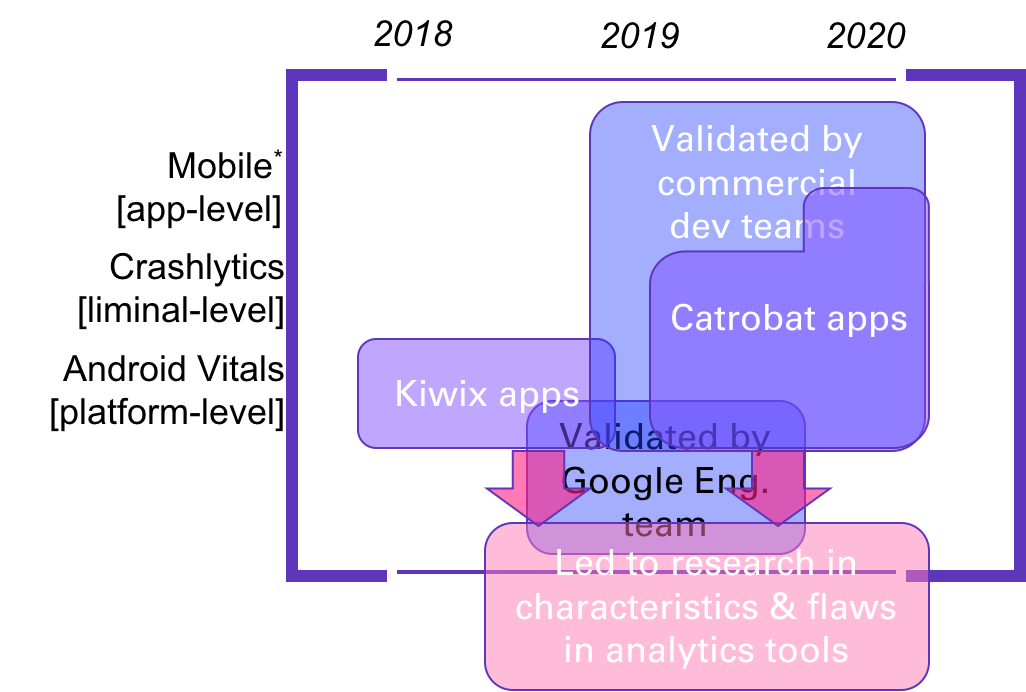
\includegraphics[width=10cm]{images/visual-connections-in-research.png}
    \caption{Visual Connections in my research}
    \label{fig:visual-connections-in-research}
\end{figure}

\textit{MUST-DO update this figure, it is out of date.} Figure \ref{fig:visual-connections-in-research}  aims to provide a visual overlay of the main practical elements of the research from 2018 to 2020. There are three main factors: 1) the type(s) of analytics used, 2) the development team and their apps, and 3) the progression of the case studies, as they augment what has been learned in earlier case studies.
% \akb{Why is it important to understand the timeline here - what implication does it have for understanding the research problem?}

The research started with the Kiwix~\footnote{The Kiwix project enables people to use Wikipedia and other content offline~\url{https://www.kiwix.org/en/}} set of Android apps where the app with the highest crash rate, as reported by Google's Android Vitals, was used as the experiment to see if the crash rate could be improved. By design the Kiwix apps do not include any analytics or crash reporting to minimise the digital usage footprint of these apps as they may be used in areas of the world where Wikipedia is banned, \emph{etc.} where the users may be persecuted or even imprisoned. Nonetheless, as the apps were available through Google Play (amongst many sources), the development team received ongoing reports in Google Play Console including the Android Vitals reports on various `stability' metrics as defined and applied by Google.

The Catrobat team was and is an extremely well researched and supported collection of mobile apps intended to help young people learn how to enjoy developing games visually. It was established % Removed details for the review period: "by Professor Wolfgang Slany of" 
at the TU Graz university where both undergraduate and postgraduate students actively practice software skills on the codebase. My engagement started around June 2019, and we decided jointly to pick the thornier and most complex Android app - Pocket Code - as the subject for our collaboration and research, as it had proved to have an intractable ongoing issue with the high reported crash rate and was therefore a worthy challenge for the concepts proposed in my research. We had a reference app, called Pocket Paint, which had a lower crash rate. Note: Pocket Paint was and is incorporated into Pocket Code in addition to being a standalone app.

Pocket Code already incorporated one of the most popular crash analytics library called Crashlytics. At the time, it used an older, mature version of Crashlytics branded Fabric (a business first acquired by Twitter, then by Google). I have chosen to use the term \emph{liminal}~\footnote{\url{https://www.lexico.com/en/definition/liminal}} to indicate crash reporting is something that lives in the boundary layer between the app and the operating system, or platform. Either is able to observe application crashes, and for apps where both the app and the platform capture information about crashes the two data sources can be usefully cross-referenced and compared, as my research has done.

As Pocket Code was an Android app, available in Google Play, the team also received the reports provided by Google through Google Play. These two data sources provided an interesting and rich set of research challenges. 

Relatively recently, in February 2020, the Catrobat team had to migrate their Crashlytics reporting from the Fabric service, which Google was ceasing, to Firebase, the replacement reporting service Google provided. In parallel with this migration of the reporting, the project team agreed to incorporate mobile analytics into their Android and iOS apps. They decided to use Firebase Analytics for various reasons (to be covered later in my thesis), hence the extension of the apps into app-level analytics.

The two arrows in the figure indicate an area of unplanned research: 
%
I discovered various flaws in the developer-oriented reports Google provides to app developers who make their apps available in Google Play (approximately 2.9 million apps globally). This led initially to discussions with the relevant engineering teams for Google Play and Android Vitals at Google where they confirmed various flaws. They asked for ongoing updates on my findings and requested a report which I provided. Through our interactions and discussions, I realised the merit of researching the characteristics and flaws in analytics tools, and particularly those provided by Google for Android developers. This research is ongoing and intended to continue post-PhD given the importance and relevance of the topic.

In mid-2019 several commercial Android development teams learned of my research and offered to contribute their experiences and practices of using mobile analytics in their commercial apps. These apps include app-level analytics in addition to the development teams receiving the ongoing reports Google provides automatically. The contributions of these development teams helped provide additional weight to the value and relevance of using mobile analytics to identify flaws in mobile apps and evidence of the importance developers placed on addressing quality issues gleaned through these tools.

%\yy{The practical research}{Need to complete the sentences, what is liminal? Change Kiwix/Catrobat apps to "Kiwix/Catrobat teams"? }

\begin{table}[htbp!]
    \centering
    \small
    \setlength{\tabcolsep}{4pt} %% default is 6pt
    \begin{tabular}{llrr}
      Case Study &Role of Researcher &Apps &Active Users\\
      \hline
       \href{https://play.google.com/store/apps/dev?id=9116215767541857492&hl=en_GB}{Kiwix}  &Embedded &18 &367K\\
       \href{https://play.google.com/store/apps/developer?id=Catrobat&hl=en_GB}{Catrobat} &Guide &6 &200K\\
       \href{https://play.google.com/store/apps/dev?id=7665838187257770408}{Greentech Apps} &Observed &10 &987K\\
       \href{https://play.google.com/store/apps/developer?id=Moonpig.com&hl=en_GB}{Moonpig.com} &Observed &1 &130K\\
       \href{https://play.google.com/store/apps/details?id=boundless.moodgym&hl=en_GB}{Moodspace app} &Interviewed &1 &20K\\
       \href{https://play.google.com/store/apps/details?id=com.localhalo.app&hl=en_GB}{Local Halo app} &Observed &1 &1.1K\\
       Commercial case study &Consultant &1 &1.9M\\
       Analytics tools &Various &10\textsuperscript{6} &10\textsuperscript{9} \\
    \end{tabular}
    \caption{Project teams and Commercial apps in the case studies}
    \label{tab:case_studies}
\end{table}

For the Kiwix case study, the researcher has been an intrinsic long-term member of the diffuse project team, able to work directly with the code-base and collaborate directly with the developers and ancillary members of the project team. The second phase of the case study included collaboration during a week-long hackathon, the first of two case studies that used a hackathon as part of the research. 

For the Catrobat case study, the researcher advised and assisted the project team to apply mobile analytics to their larger, older, and less reliable app: \emph{Pocket Code}. The researcher helped lead a one-day hackathon and otherwise interacted through a bug reporting tool, JIRA, discussions and using shared documents. Pocket Code also included a crash-reporting library which allowed cross-tool comparisons of reports, analytics and data. During the research, the reporting platform for the crash-reporting was migrated to a newer service which provided further insights and comparisons across and between the various mobile analytics tools.

The Greentech apps case study blends public and private sharing of their projects, they track issues in public, the codebase is private. Their active userbase is larger than the combined userbases of the Kiwix and Catrobat mobile apps. The team structure is similar to those for the Kiwix project: it is a not-for-profit foundation where donations help fund some of the development work; however many of the development team members are part-time volunteers. Their core team are in Bangladesh, distant from the Western world, and their focus is to enable native Bangla speakers to learn and study the Quran. Their priorities differ from those of most projects; the quality of their material is paramount; and they sometimes disable support for apps that have serious quality flaws in these materials. 

For the commercial app teams (Moonpig, Moodspace, and LocalHalo), the researcher corresponded with one of the development team for each of the commercial apps and received either direct access to their analytics tools (LocalHalo), or was provided with snapshots (Moonpig and Moodspace). Permission was granted by their respective organisations for their contributions to be used for research purposes.

The corporate case study has an order of magnitude more complexity than the other apps with much higher demands on the software being reliable and performant. The business and the service provided through the client apps are expected to grow massively as the product matures and the software quality improves. While they include clients for MacOS, iOS, Android, webRTC, and Windows desktop operating systems, the case study focuses on the Android client.

How developers of Android apps actually use mobile analytics for remote logging compared to how developers use local logging focuses on the perceived purpose of the logging across over 100 opensource projects on GitHub.com. And the final case study is from the perspective of a startup who are developing and researching tools and techniques to help developers improve their design, implementation and use of usage analytics tools (both web and mobile apps). 

\subsection{TODO: Structure used to describe the case studies}
TODO describe Arosha's proposed structure and introduce its applicability and purpose here.


\section{Research ethics for the case studies}
\label{section-research-ethics-for-the-case-studies}

MUST-DO complete this section and have it cross checked with my supervisors.

\begin{itemize}
    \item Ethics review for Workshop in Poland (and then for various reasons the contents of the workshop were not viable because of the effects of COVID-19.
    \item No other human subjects, the data related to apps and how the app is used and performs, humans are not the subject of the research.
    \item Opensource, freely available apps without any restrictions on sharing the findings of the performance of the apps. No PII information collected by the analytics tools used.
    \item Semi-structured interviews with various individuals 
\end{itemize}

Participants were briefed and gave their permission either individually or on behalf of their organisations to use the material they freely provided. Several have reviewed my research and provided constructive feedback which has been applied. It has not always been practical to reach them, for instance some are no longer reachable. None of the analytics information provided contains PII. 
\clearpage


%\setcode{utf8}

\section{Kiwix Android Apps}
\label{section-kiwix-case-study}
Relying on analytics and reports provided by the Google Android's platform and presented in Google Play Console, we were able to reduce the crash rates of a family of Android apps. 
%
We chose the most sophisticated and complex of the Android apps, which also had the highest Crash rate at the time (see Table~\ref{tab:gpc_kiwix_apps_11_feb_2019}). The reduction went from over 5\% to under 0.25\% during the case study.

Figure~\ref{fig:android-vitals-kiwix-android-crash-rate-vs-peers} provides an illustrative example of the crash rate for Kiwix Android. The comparison with its peers, apps in the same category across Google Play, also shows Kiwix Android was in the bottom 7\% in terms of crash rate in that category. So the app was unreliable by either measure.

By applying what the team learned about crashes reported in Android Vitals the team was able to reduce the crash rate of this app several fold. When the improved codebase was used to refresh various custom apps their crash rates also decreased several fold.

\begin{figure}
    \centering
    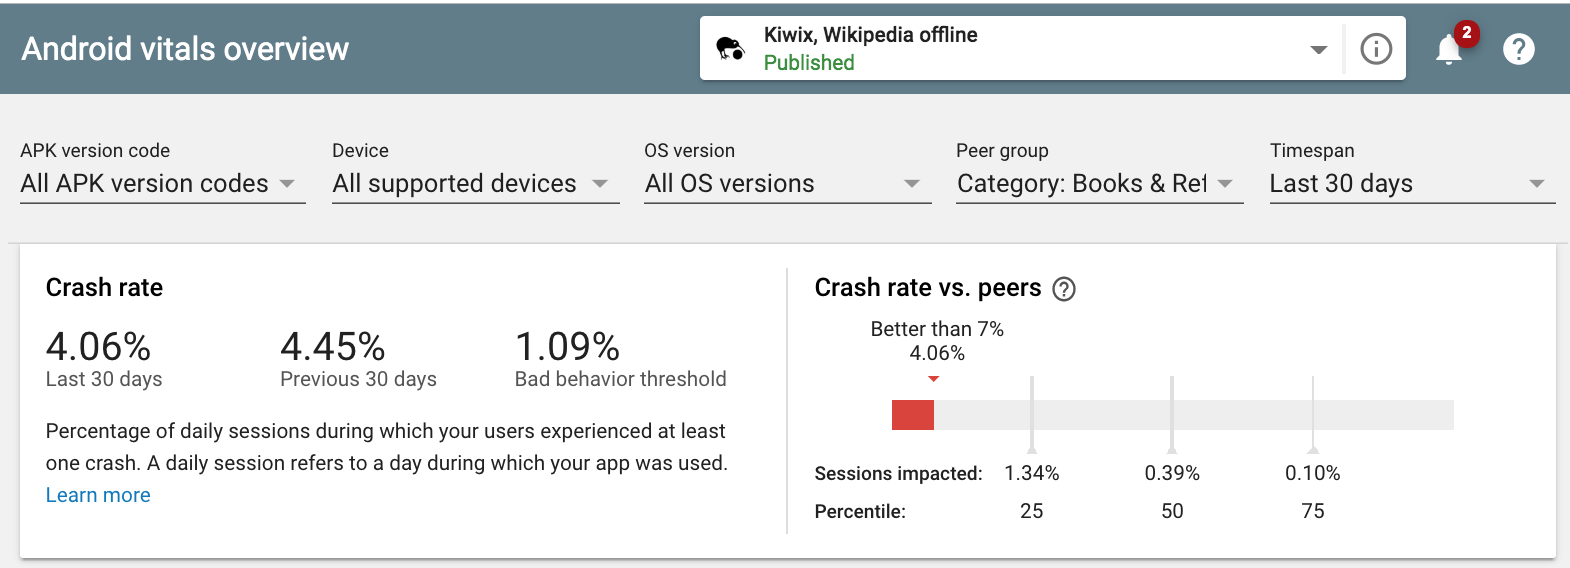
\includegraphics[width=13cm]{images/android-vitals-screenshots/Example-crash-rate-vs-peers 10-jun-2019.png}
    \caption{Android Vitals Kiwix Android crash rate vs peers \nth{10} June 2019}
    \label{fig:android-vitals-kiwix-android-crash-rate-vs-peers}
\end{figure}

Note: I have been involved in various aspects of Kiwix since 2014 including helping with the Android app, with manual and automated testing, with the PHeT project mentioned here, and so on.

\setminted{fontsize=\small,baselinestretch=1}

\subsection*{Evidence}
  \begin{minted}[
    gobble=4,
    frame=single,
    fontsize=\tiny,
    breaklines=true
  ]{yaml}
    evidence available :
      vitals-scraper : ~/sandbox/vitals-scraper-logs/android-stability-analysis/data/from-android-vitals
      google-play-console-reports : ~/Dropbox/Google Play Console Reports/reports/catrobat/pocketcode/crashes
      various-materials : in Dropbox
      co-written-paper : MOBILESoft 2019~\citep{harty_google_play_console_insightful_development_using_android_vitals_and_pre_launch_reports}, WAMA 2019~\citep{harty_better_android_apps_using_android_vitals}, MOBILESoft 2020~\citep{harty_improving_app_quality_despite_flawed_mobile_analytics}, ICST 2020~\citep{harty2020_how_can_software_testing_be_improved_by_analytics_to_deliver_better_apps}.
    evidence-needed : 
      Supporting materials for Phase 2:
      Supporting materials for Phase 3: 
      Releases and their release dates.
      Latest status of the tickets related  to crashes and ANRs.
      Current stability metrics for the Kiwix apps.
  \end{minted}

\subsection{Introduction of Kiwix Android Case Study}
%Introduce Kiwix at the risk of repetition. 
% TODO replace URLs with citations.
Kiwix makes knowledge available to people with no or limited internet access (\emph{i.e.} four billion people) by providing highly compressed content and a reader for the bespoke compression format. Anyone is free to use the software and the content. The project includes an offline reader for online content like Wikipedia, Project Gutenberg, or TED Talks and the project also develops and maintains software to download, compress, package, and make content easy to download and share~\citep{kiwix_about_the_project, gomez2017_wikimedia_kiwix_article}.

The project provides offline access to Wikipedia materials and many other read-only materials including TED talks, StackExchange sites, interactive science simulations, and others~\citep{kiwix_about_the_project, gomez2017_wikimedia_kiwix_article}. 

The Android project comprises various apps all based on a common opensource codebase. The core case study captures activities from early 2019 to early 2020; however the project is a long-term, ongoing project and I am still involved with it. Several post case-study updates will be covered in later chapters. The crash rate had been excessive for over a year and far exceeded the bad behaviour threshold Google Play specified. 

The case study started with a period of observation and discussion of the crash rate in particular as it had increased repeatedly and to such an extent that the 2.3 release had been aborted by the project team, various details follow.

In mid-April 2018 the reported crash rate was 1.53\%~\footnote{Details available in \href{https://github.com/kiwix/kiwix-android/issues/712}{issue 712} for the Kiwix Android project, the main app releases were version 2.2 and 2.3 at the time.}. By mid-June 2018 the overall crash rate had increased to 1.71\%~\footnote{The crash rate for version 2.2 was 2.03\% in the 30 days to \nth{14} June 2018.}. The rollout for 2.3 was aborted in February 2019~\footnote{The milestone for this release and the issues that were addressed is available online~\url{https://github.com/kiwix/kiwix-android/milestone/1?closed=1}.} as there was a crash that affected 10\% to 20\% of the users (according to the lead developer at the time). The crash rate for the app averaged over 5\% in January and February 2019. 


%\akb{Provide dates over which the excessive crash rate was noted? Also, while the project is a long-term, ongoing project, your case study captures its activity during a specific window.}

The project team actively exclude any tracking or analytics within the app to minimise the risk of harm to users of the app. This is because in some parts of the world Wikipedia is banned \url{https://en.wikipedia.org/wiki/Censorship\_of\_Wikipedia} and usage may result in oppression, prison, and so on. By design the app makes Wikipedia content freely available and easy to distribute peer to peer (and it has been downloaded in response to bans of the main Wikipedia web site~\url{https://twitter.com/KiwixOffline/status/968493031224733697?s=20}). The apps are also available on Google Play and the apps are popular there. The project team agreed they were willing to use the analytics Google Play provides about their apps and these analytics provide the basis for this case study.

Google Play obtains, processes, and provides analytics of Android apps from opted-in devices that incorporate Google Play Services (installed over 10 billion times \url{https://play.google.com/store/apps/details?id=com.google.android.gms&hl=en\_GB&gl=US} and installed on several billion Android devices (\url{https://en.wikipedia.org/wiki/Android_(operating_system) 2B+ in 2017}). These analytics include stability metrics for Android apps on those devices where developers are provided the analytics for their apps free of charge.
Note: Google Apps are available to download from third-party websites, particularly \url{https://www.teamandroid.com/gapps/}. 


The development team was relatively large and fluid ranging from teenagers to several professional developers and their active contribution periods ranged from weeks to many years~\footnote{Kiwix Android had 96 Contributors to the GitHub project at the time of writing~\url{https://github.com/kiwix/kiwix-android/graphs/contributors}}. The developers reviewed the code using pull requests.  The codebase included some application level automated tests; and the project included a continuous build, and used a commercial device farm provided free of charge by bitbar.com~\footnote{The tests were run using BitBar's custom \href{https://support.smartbear.com/bitbar/docs/integrations/gradle.html}{Gradle plugin} BitBar also providesinteractive testing on a wide range of devices, which helps with \emph{ad-hoc} testing, \href{https://github.com/kiwix/kiwix-android/pull/2350}{Issue 2350} provides a good example where the developers needed to test on a range of Android releases and had the facility to use this service.} 

One of the apps was chosen as the experiment and another as the control to determine whether the crash rate could be reduced through applying information Google Play provides in Google Play Console.

This was the first of the case studies and opened the research into the effects of applying analytics gathered at the platform (Android) level. Key distinctions include: the ability to perform a controlled experiment, to then see results of what happened when the experiment’s code was rolled out to the rest of the sibling apps, and the long terms effects of pursuing crashes and fixing them over a series of releases.

Key similarities include the use of Google Play Console analytics (virtually all the projects use it to varying degrees), and the improvements (reductions) in failures through applying the techniques. 

%\akb{I like this summary of the key differences and similarities}

\subsection{Context}
\textit{(Product/Project overview, Developer characteristics, tools, methods, key challenges for product/project).}

\subsubsection{Product/Project overview}
The Kiwix project was created in 2006 to help ensure people can access the \emph{``sum of all human knowledge"}~\citep{coillet2016-wikimedia-kiwix-ten-years}. Annually over a million people download it and the content packages the project creates and provides free of charge~\citep{coillet2016-wikimedia-kiwix-ten-years}.

It is mature as a project and led by several highly experienced contributors, where two volunteers co-founded the project and others joined over the years. From the outset the project has been open, and the software is also open sourced~\citep{sutherland2014_wikimedia_on_kelson}. It has received various grants and awards to help sustain the project and some of the funds pay for a hybrid mix of developers, where some are paid for at least some of their contributions. The Android codebase is one of many maintained by the project~\citep{gaudin2017_wikimedia_kiwix_android}. 

Various codebases, including Android, use and depend on another codebase written in C++ to process the custom ZIM file format developed by and for this project~\citep{gaudin2017_wikimedia_kiwix_android}. The open ZIM project (\url{https://wiki.openzim.org/wiki/OpenZIM}) and codebases are closely related and integrated with the Kiwix project and codebases, nonetheless it is distinct and separate.

\subsubsection{Design of the Kiwix family of apps}
Here is a brief overview of the relevant history of the codebase when the case study started. .

\begin{comment}
Additional material on Kiwix custom apps - possibly put in an appendix?

The project created a distinct opensource project for the creation of Android custom apps~\url{https://github.com/kiwix/kiwix-android-custom} At the time of the case study the build tools were very immature for custom apps.

\url{https://github.com/kiwix/kiwix-android-custom/blob/master/CONTRIBUTING.md}

\end{comment}



The Kiwix Android project was started in 2013 as a port of one of the other Kiwix codebases; and version 1.0 of the App was released in Google Play in Spring 2013~\footnote{\url{https://sourceforge.net/p/kiwix/kiwix/ci/1.0-google-play/tree/android/}}. The app was designed to enable people to read contents provided in a custom file format called ZIM files. Users originally needed to obtain and transfer these files onto their Android devices, the app was then enhanced with the addition of a custom downloader designed to suit the needs of users who may have intermittent, sometimes expensive, and unreliable internet connections. The custom downloader allowed users to pause downloads and to continue partial downloads.

The project team also realised that some users would prefer versions of the app that included pre-packaged contents, such as Wiki Medicine articles, travel articles, and so on, all drawn initially from Wikimedia Foundation websites and content. This led to the development and release of various custom Android apps. The build process for custom apps was quite manual and few members of the team ever knew how to create and package existing custom apps, let alone create custom apps with new contents.  In parallel we devised tools and processes to package the HTML5 PHeT simulations in 2015/16 and then created and released a custom app containing these simulations. The pre-packaged content was packaged using standard Google Play Android functionality known as \href{https://developer.android.com/google/play/expansion-files}{APK Expansion Files}~\footnote{Google announced material changes to the mechanism from August 2021:~\emph{``Important: From August 2021, new apps will be required to publish with the Android App Bundle on Google Play. New apps larger than 150 MB are now supported by either Play Feature Delivery or Play Asset Delivery."}~\citep{apk_expansion_files}}. % A copy of the current contents of this guide as of 5th June 2021 has been stored with the rest of the supporting materials as the contents are likely to change in the coming months...

The custom apps did not need the custom downloader or the code that searched for ZIM files on the Android device as they came with their own pre-packaged content.


\subsubsection{Developer characteristics}
One of the many benefits of the project’s openness is the visibility into the developers who have developed and maintained the source code \url{https://github.com/kiwix/kiwix-android/graphs/contributors}. Many of the contributors joined as volunteers through Google Summer of Code~\citep{google_summer_of_code} or Google Code-in \url{https://codein.withgoogle.com/archive/}~\footnote{Google Code-in was shutdown and the history archived by Google in 2020.}, and several of these became core contributors for a year or more, and some of these now work for leading technology businesses. 

Life-members: the two co-founders of the Kiwix project also contribute to the codebase at times. They are both long-term software developers across various programming languages and codebases.

Professional developer: sufficient funds were made available to fund a professional Android developer for a period of just under 20 months. (Severe cutbacks in funding as part of the manifold effects of COVID-19 restrictions ceased their involvement).

Miscellaneous contributors: including me, and several people I introduced. Occasionally Software Engineers from Google contributed their time to help the project, for instance as part of what Google call Google Serve~\footnote{(I used to be involved in Google Serve when I was an employee of Google from 2006 to 2010.)}.

%\akb{You will need to tidy up the language to be consistent in how you refer to yourself - e.g., I am not sure if 'author' and you are the same person in the paragraph above - would be best to write in 3rd-person as far as possible}

The vast majority of the contributors had developing for Android as a primary interest, unsurprising as this is the Android app for the project.

\subsubsection{Tools}
For the case study the main measurement tools we used were Google Play Console and Android Vitals in particular. Standard, commonplace Android Development tools such as Android Studio https://developer.android.com/studio (the default IDE) were and are used by the developers. The source code was and is hosted on GitHub \url{https://github.com/kiwix/kiwix-android}.

%\akb{Main tool or tools?}

\subsubsection{Related tools}
The software development tools suited a large mainstream Android opensource project, i.e. the tools and services were free-of-charge. Many are provided by commercial organisations such as Google, GitHub, Travis-CI, and \href{https://bitbar.com/}{BitBar} (since acquired by \href{https://smartbear.com/}{SmartBear}). Often the tools are popular and widely used, e.g. Junit and Espresso frameworks for the automated tests. The project uses continuous builds, at the start of the case study it used travis-ci the project migrated to GitHub actions in late 2019, early 2020 \url{https://github.com/kiwix/kiwix-android/issues/1593}.

The Kwixi Android project uses various frameworks and libraries, many are listed in the project README~\url{https://github.com/kiwix/kiwix-android} (e.g. Espresso isn’t listed, however it’s used by the project \url{https://github.com/kiwix/kiwix-android/search?q=espresso}).

Code coverage is tracked automatically online using a free service called Codecov \url{https://codecov.io/gh} The line coverage according to this tool ranged between roughly 32\% and 43\% \url{https://app.codecov.io/gh/kiwix/kiwix-android}~\emph{i.e.} where there are one or more automated tests that execute a given line of source code.  

The codebase could be built from a fresh installation from the source on GitHub.com; This is mentioned as relatively few projects can actually be compiled and built as-is. There had been significant investment in establishing the vanilla build process (which relied on several binaries being pre-built as part of sibling projects).

The resources used in the app are translated using translatewiki.net which also supports many other projects \url{https://translatewiki.net/wiki/Translating:Kiwix} and \url{https://diff.wikimedia.org/2011/08/20/kiwix-localisation-is-supported-at-translatewiki-net/}.

The project, and various related projects, are automatically built on a nightly basis and made freely available online \url{http://download.kiwix.org/nightly/}.

\subsubsection{Methods}
%\emph{[I’m not sure what this topic should include – should it be the methods applied in the case study? or those applied by the project/product team? Both? or something else entirely?] Anyway, I’m writing some notes on the methods used by the development team.}

The development team had few of the practices considered part of Agile development – no sprints, no scrum master, no story points, etc. Nor was it waterfall, so few signs of requirement documents, test plans, and so on. The project did and does use 3 templates on GitHub to help organise new work requests \url{https://github.com/kiwix/kiwix-android/tree/develop/.github/ISSUE\_TEMPLATE} and occasionally created small lightweight projects \url{https://github.com/kiwix/kiwix-android/projects?query=is\%3Aclosed} 

However as mentioned in the Tools topic, the project did have some automated tests, a CI, used pull requests, code coverage reports, a public issue tracker, code reviews, and so on.

Several key contributors had at least read-only access to Google Play Console for one or more of the apps. I have had read-only access to the organisation’s Google Play Account for several years (access at the organisation level enables access to download monthly reports in addition to viewing the details of any of the particular apps).

The set of project members on GitHub.com is updated from time to time, probably a couple of times a year (For example, I am no longer currently a member as of the end of December 2020 as I didn’t contribute any code in 2020).

\subsubsection{Key challenges for the product/project}
\textit{[Here my focus is mainly on technical challenges. Let me know if you’d like me to cover other challenges.]}

Few of project contributors want to write tests, sort out build or testing infrastructure, or fix bugs. Although the project did run the automated tests on several physical devices there was marginal perceived value in doing so, and few of the development team had access to the testing service which further discouraged their involvement in the automated tests as they couldn't see the tests running or the test results~\footnote{(It wasn’t practical to materially expand who could access the service provided by Bitbar which was oriented more towards paying customers. Access to the service was donated as a favour to me).}.

%\akb{How is the parenthetical point / last sentence relevant to the research?}

Many new volunteer contributors want to contribute new code rather than maintain existing code, especially existing code where failures lurk. 

\subsection{Analytics intervention}
\textit{(Describe what you did with analytics in the context of the case). Focus on this and the next sections since they’re core to the thesis.}

Analytics was used to select which app(s) to focus on, to determine the replacement of high-functionality/low-reliability custom code with low-functionality/high-reliability code, and to prioritise the crash clusters to address over several releases of the experiment/treatment app. It was also used to measure the effects of the analytics interventions.

\begin{itemize}
    \item Google Play Console provided details of the install base for the various Kiwix Android apps and it also provided a dashboard for each of these apps, these sources were used to help select which apps to focus on - those that were popular and would have lots of data.
    \item Android Vitals was used to provide the other information, on the custom downloader code and to determine which crash clusters to focus on.
\end{itemize}

%\akb{Check consistency with paragraph above where both Google Play Console and Vitals were mentioned as the main measurement (i.e. analytics?) tools.}

\href{glossary_android_vitals}{Android Vitals} was the source of the analytics for this case study. It provided statistics and details of crashes for the more popular Kiwix Android apps; as we discovered Android Vitals does not provide statistics or reports for the less popular apps; why this occurs will be discussed in the \href{case-study-kiwix-discussion}{Discussion section} of this case study. 

%\akb{As noted above, it would be good to have dates over which the observations recorded in the case study were recorded so that the reader understands when 'the start of the case study' was}

At the start of the case study, in February 2019, all the apps had a crash rate above Google's Bad Behavior Threshold of 1.09\% as Table~\ref{tab:gpc_kiwix_apps_11_feb_2019} illustrates. The total count of active installs was 252,490 according to Google Play Console with the core Kiwix app the most popular with 101,873 installs, followed by WikiMed in English with 55,357 installs, and then Chemistry \& Physics simulations with 37,244 installs. All the apps were very highly rated, ranging from 4.74 to 4.43 stars~\footnote{Google announced changes to the rating calculations in May 2019~\citep{androiddevelopersblog2019_io2019_whats_new_in_play}. Developers were able to see both the current and the new ratings for several months in Google Play Console before Google rolled out the new ratings to the public facing store front of Google Play. These changes mean ratings pre and post Summer 2019 are not safe to compare directly.}.

The reported crash rates were compared for the core Kiwix app and various custom apps. Kiwix had the highest crash rate, followed by the PHeT application\footnote{The PHeT application has since been renamed \href{https://play.google.com/store/apps/details?id=org.kiwix.kiwixcustomphet}{Chemistry and Physics simulations}. The content source,~\href{https://phet.colorado.edu/}{University of Colorado Boulder}, have since released their own Android app, called~\href{https://play.google.com/store/apps/details?id=edu.colorado.phet.androidApp}{PhET Simulations}, and the Kiwix team agreed to rename our app to enable their app to be more easily discovered by new users of either app. The contents were and still are freely available to be used~\url{https://phet.colorado.edu/en/licensing}. For completeness, I was involved in some of the initial work for this project and also contributed translations and support to the upstream PHeT project.}.
%
The rest of the custom applications had a range of crash rates from 1.77\% to 1.13\% (Table~\ref{tab:gpc_kiwix_apps_11_feb_2019}).

\begin{table}
    \centering
    \tabcolsep=0.06cm
    \tiny
    \begin{tabular}{lrrrrrr}

	App name &Active Installs & Average rating & Total ratings & Crashes & Crash Rate & Last Update \\ 
	%\begin{CJK*}{UTF8}{bkai}醫學維基百科(離線版)\end{CJK*} &  &  &  &  &  &  \\ 
WikiMed (in Chinese)  &  &  &  &  &  &  \\
	org.kiwix.kiwixcustomwikimedzh & 3,297  & 4.45 & 220 & 31 & NA & Sep 6, 2018 \\
	%\begin{CJK*}{UTF8}{gbsn}医療ウィキペディア(オフライン)\end{CJK*} &  &  &  &  &  &  \\ 
	WikiMed (in Japanese)  &  &  &  &  &  &  \\
	org.kiwix.kiwixcustomwikimedja & 1,498  & 4.63 & 27 & 46 & NA & Sep 6, 2018 \\ 
	% ମେଡିକାଲ ଉଇକିପିଡିଆ (ଅଫଲାଇନ
	Wiki Medicine (in Odia) &  &  &  &  &  &  \\ 
	org.kiwix.kiwixcustomwikimedor &242  & 4.72 & 102 & 3 & NA & Sep 9, 2018 \\ 
	%ویکی‌پدیای پزشکی آفلاین &  &  &  &  &  &  \\ 
    Wiki Medicine (in Farsi) &  &  &  &  &  &  \\ 
	org.kiwix.kiwixcustomwikimedfa &2,935  & 4.60 & 610 & 5 & NA &  Sep 20, 2018 \\ 
%	ويكيبيديا الطبية بلا إنترنت &  &  &  &  &  &  \\
	Wiki Medicine (in Arabic) &  &  &  &  &  &  \\
	org.kiwix.kiwixcustomwikimedar &11,940  & 4.65 & 2477 & 424 & 1.77\% & Sep 12, 2018 \\ 
	WikiVoyage Europe - Offline Travel Guide &  &  &  &  &  &  \\ 
	org.kiwix.kiwixcustomwikivoyageeurope &712  & 4.65 & 59 & 0 & NA & Dec 16, 2018 \\ 
	Wikivoyage - Offline Travel Guide &  &  &  &  &  &  \\ 
	org.kiwix.kiwixcustomwikivoyage &5,680  & 4.73 & 706 & 71 & 1.22\% &Dec 16, 2018  \\ 
	WikiSpecies &  &  &  &  &  &  \\ 
	org.kiwix.kiwixcustomwikispecies &141  & 4.58 & 43 & 0 & NA & Sep 11, 2018 \\ 
	WikiMed mini - Offline Medical Wikipedia &  &  &  &  &  &  \\ 
	org.kiwix.kiwixcustomwikimedmini &8,883  & 4.58 & 507 & 343 & 1.5\% &  Aug 31, 2018 \\  
	WikiMed - Wikipedia Medizin (Offline) &  &  &  &  &  &  \\ 
	org.kiwix.kiwixcustomwikimedde &5,174  & 4.74 & 259 & 56 & NA &  Dec 16, 2018 \\ 
	WikiMed - Wikipédia médicale hors-ligne &  &  &  &  &  &  \\ 
	org.kiwix.kiwixcustomwikimedfr &12,163  & 4.68 & 1674 & 832 & 1.19\% &  Sep 4, 2018 \\  
	WikiMed - Wikipédia Médica Offline &  &  &  &  &  &  \\ 
	org.kiwix.kiwixcustomwikimedpt &347  & 4.71 & 95 & 10 & NA & Dec 16, 2018 \\ 
	WikiMed - Wikipedia Médica Offline &  &  &  &  &  &  \\ 
	org.kiwix.kiwixcustomwikimedes &4,947  & 4.74 & 760 & 326 & 1.83\% & Dec 16, 2018 \\
	WikiMed - Offline Medical Wikipedia &  &  &  &  &  &  \\ 
	org.kiwix.kiwixcustomwikimed &55,357  & 4.69 & 16685 & 2810 & 1.13\% & Sep 6, 2018 \\ 
	Kiwix, Wikipedia offline &  &  &  &  &  &  \\ 
	org.kiwix.kiwixmobile &101,873  & 4.52 & 14427 & 12140 & 5.07\% & Aug 8, 2018 \\ 
	Encyclopédie de la Tunisie &  &  &  &  &  &  \\ 
	org.kiwix.kiwixcustomtunisie &27  & 4.43 & 7 & 3 & NA & Sep 22, 2018 \\ 
	Enciclopedia de Venezuela &  &  &  &  &  &  \\ 
	org.kiwix.kiwixcustomvenezuela &30  & 4.63 & 8 & 1 & NA & Sep 11, 2018 \\ 
	Chemistry \& Physics simulations &  &  &  &  &  &  \\ 
	org.kiwix.kiwixcustomphet &37,244  & 4.65 & 1910 & 1050 & 4.08\% & Sep 24, 2018 \\ 

\end{tabular}		
    \caption{Google Play Console statistics for published Kiwix Apps @\nth{11} Feb 2019}
    \label{tab:gpc_kiwix_apps_11_feb_2019}
\end{table}					

Initial analysis of the crash rates across the Kiwix apps found several clusters in the crashes, some where common to several apps - unsurprisingly since they shared a common codebase, others were specific to a particular app. Two examples illustrate specific crash clusters:
\begin{enumerate}
    \item Crashes in the downloader - this code was only active in the main Kiwix Android app, none of the custom apps used the downloader, hence it wasn't a surprise these crashes were only reported in the main app. In Figure~\ref{fig:android-vitals-kiwix-android-example-crash-clusters-10-jun-2019} all three of most frequent crash clusters were in the download service. 
    \item Crashes in the Chemistry \& Physics simulations app. These crashes were related to the contents which was multi-layered JavaScript with deeply nested calls. The JavaScript powered the simulations and wasn't intended to run in a WebView container, WebViews and some of their effects will be discussed later in this case study and also later in this thesis in the~\href{section-webview-component}{WebView Component section}.
\end{enumerate}

\begin{figure}
    \centering
    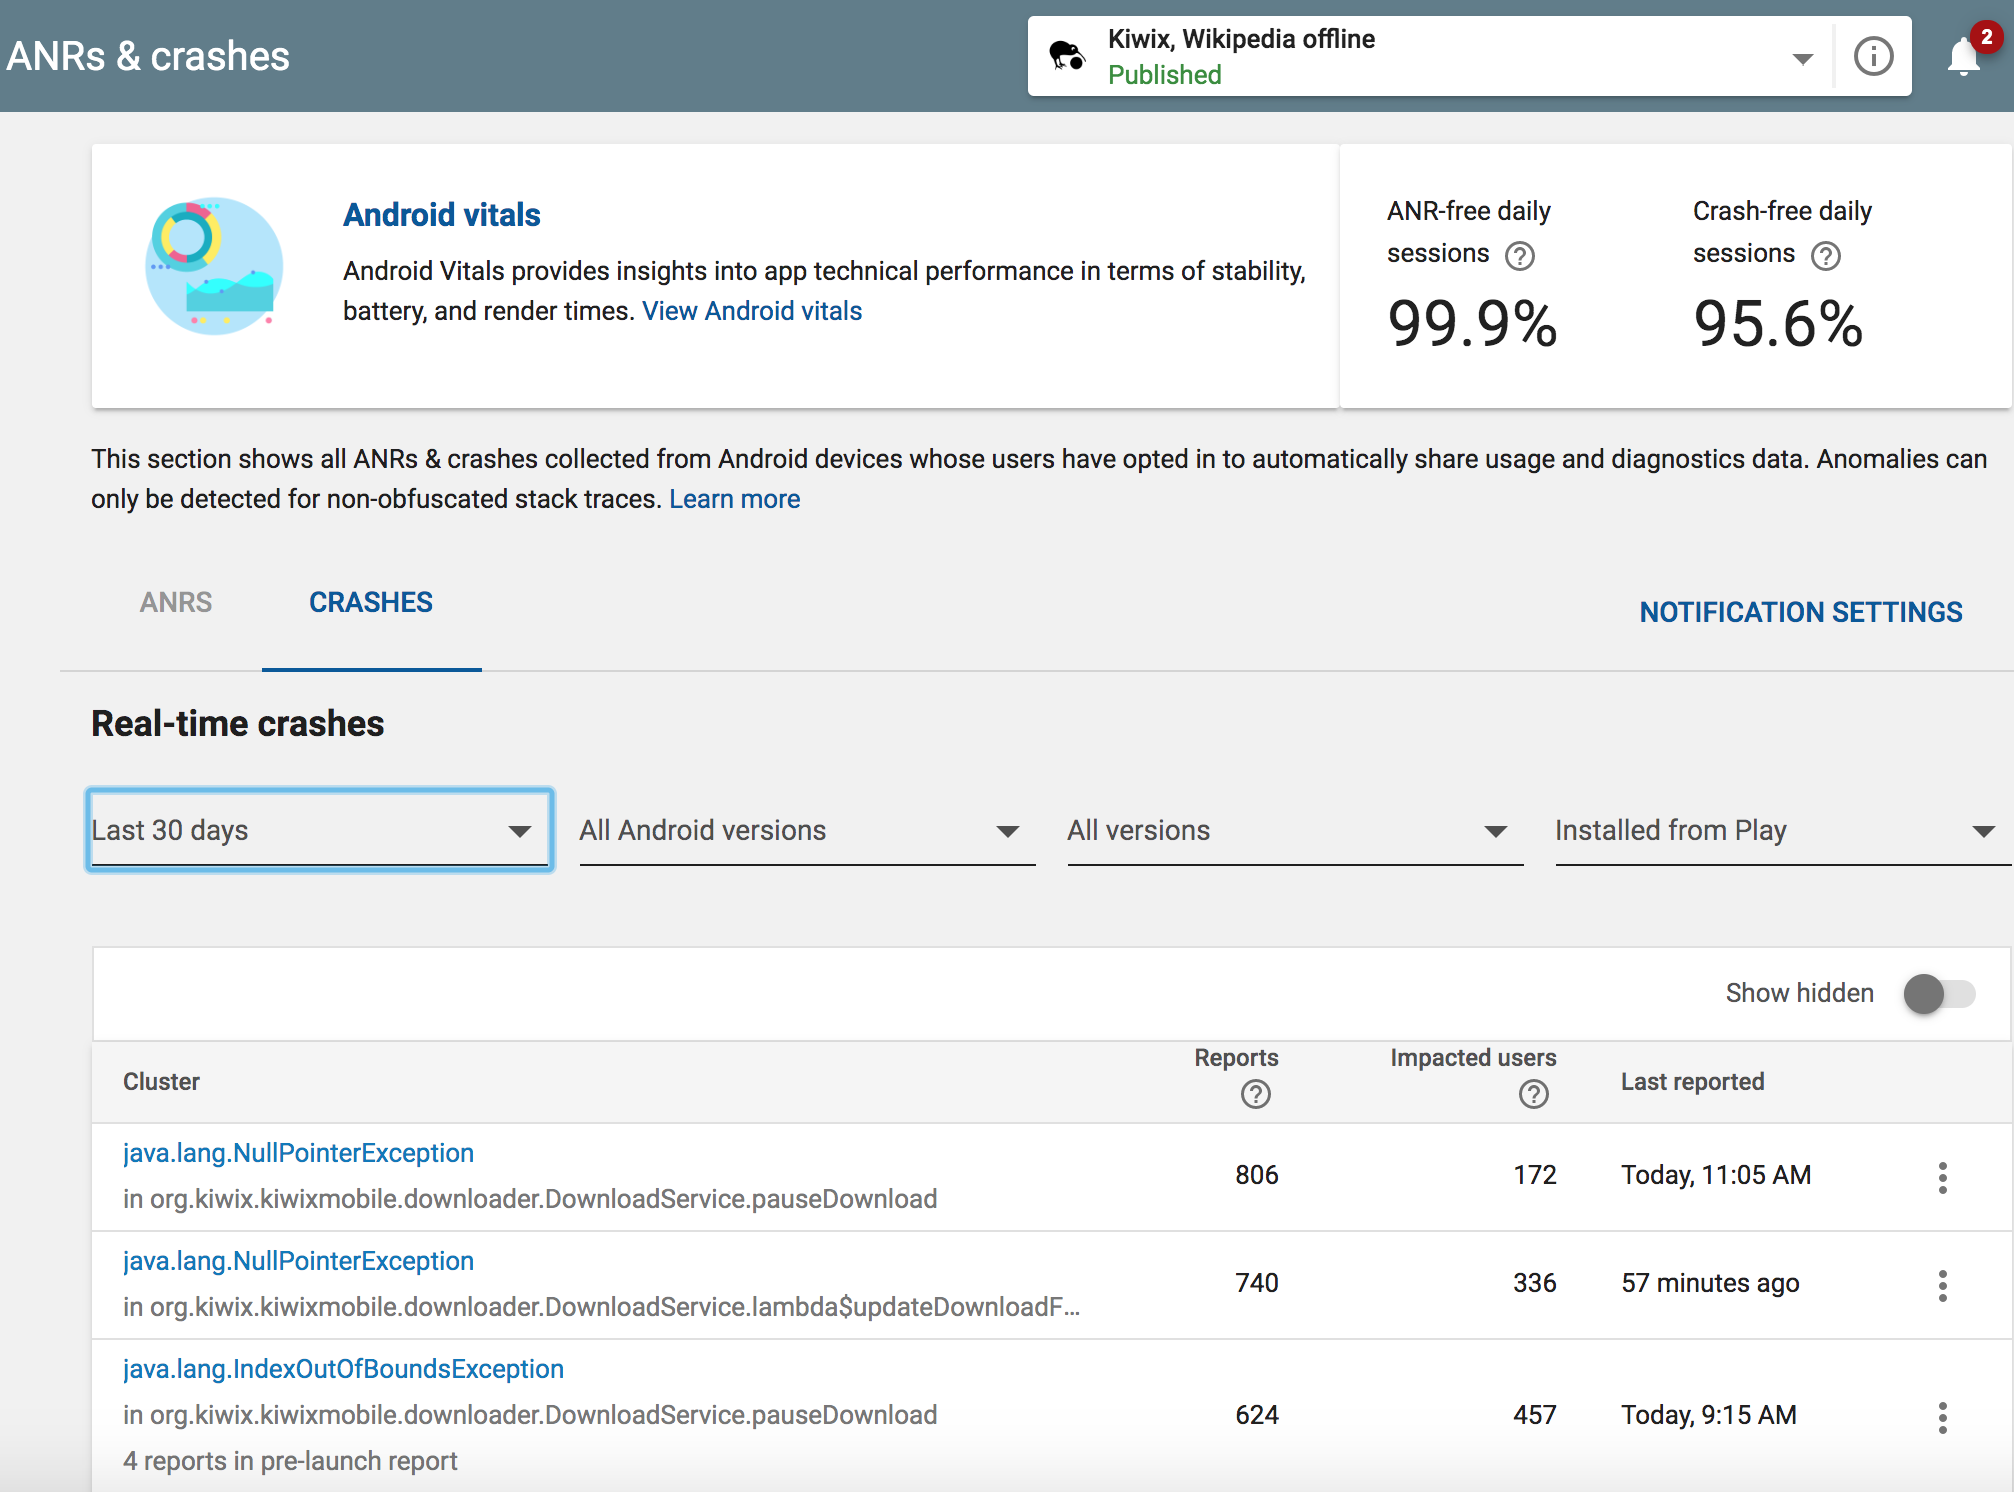
\includegraphics[width=13cm]{images/android-vitals-screenshots/Example-crash-clusters 10-jun-2019.png}
    \caption{Android Vitals: Kiwix Android crash clusters snapshot on \nth{10} June 2019}
    \label{fig:android-vitals-kiwix-android-example-crash-clusters-10-jun-2019}
\end{figure}

In March 2019, we~\footnote{The Android project leads at that time and myself} decided to focus on using analytics to effect improvements in the main Kiwix app and use WikiMed in English as the control. 
\begin{itemize}
    \item There were several reasons for selecting the Kiwix app as the experiment: it contained all the functionality\footnote{baring a tiny amount of code used in the custom apps} and it could process all the contents that the various custom apps contained therefore just about any of the current crashes could potentially be addressed through working on this app. Furthermore as the custom apps were derived from this app fixes in the codebase for the Kiwix app could percolate to the custom apps in future. 
    \item WikiMed in English was the second-most popular app in the family and was highly representative of many of the custom apps in terms of the contents and the likely usage.
\end{itemize}

We chose not to select the Chemistry \& Physics simulations as the contents were highly specific~\footnote{Furthermore, at the time the JavaScript libraries used in the simulations had high demands and would not run as-is on older Android devices. One of the Kiwix developers used a transpilation step to enable the simulations to run on these older devices, nonetheless the simulations were sometimes slow to load and less reliable than we desired. Again, all challenges that were well worth addressing (and the team did so), however they meant we chose not to use this app in the experiment.} 
and if we focused on fixing crash clusters specific to this app they may not effect improvements in the crash rates of many of the other apps in the family. (To be clear, we agreed the specific crashes were still relevant and would be worth addressing, however they weren't the main focus of the work.) 

Three bug clusters were identified through the analysis: the download manager, Android Lifecycle management, and content processing. The development lead was pressed for time and believed the causes of these bug clusters were hard to address. Various approaches were considered including paying for some off-shore developers to sift through the code for clues of the causes; however these were not followed through, partly because of the perceived complexity of a) solving the bugs, b) ensuring they were actually fixed, c) integrating with the Android platform. 
% See email conversation https://mail.google.com/mail/u/0/?q=kiwix+crash+rate+#search/kiwix+crash+rate/QgrcJHrhsvdVtDQRKfRGJrZmpsMLLCfQJcL

\subsubsection{Crash reproduction mini-experiments} 
Two mini-experiments were established during this case study with the aim of evaluating crash reproduction of crashes reported by the mobile analytics. These were: 1) testing interactively on a physical device 2) using CrashScope as the authors of that research claimed it was effective at reproducing crashes.

\textbf{Mini-experiment: device-specific interactive testing} 
Android Vitals sometimes includes the crash rate for specific device models when Google has sufficient data to publish this statistic for that device. One of the devices with a high crash rate was a sm-g532 model. This is a Samsung phone. The model code matches several branded models. As part of the research I decided to procure one of these devices to determine whether crashes could be reproduced when using this device.  

\textbf{Method}: Various sources are available online to map the model code to the branded models. For this case study \url{https://desktop.firmware.mobi/} was used, and one of the matching models was purchased: the Samsung Galaxy Grand Prime Plus Black G532 8GB. 

The then current version of Kiwix was installed on this device~\footnote{Current and historical releases of the Kiwix app are freely available online at \url{http://download.kiwix.org/release/kiwix-android/}.} and the app was used interactively with the aim of triggering one or more of the crashes being reported in Android Vitals. We were not able to explicitly reproduce any of the reported crashes during several sessions of testing over several weeks. 

\textbf{Results}: Given the volume of that testing the results are not definitive and it would be inappropriate to form conclusions from this testing. Percentages over a population of sessions do not necessarily distinguish between a subset of users who have perennial crashes consistently or crashes that occur less frequently over a larger portion of the userbase. There may be other, currently unknown contributory factors that led to the crashes for users on those device models.

\textbf{Mini-experiment: using CrashScope}
The aim of this experiment was to see if CrashScope can trigger some of the crashes automatically that are reported in Android Vitals (part of the Google Play Console). A version of CrashScope is available online~\footnote{at~\url{http://173.255.245.197:8080/CrashScope/index.xhtml}, obtained from the project's homepage~\citep{crashscope_project_homepage}}. In~\citep{moran2016_automatically_drr_android_app_crashes} the authors were able to find distinct crashes with CrashScope compared to other automated testing tools and their automatically bug-reproduction reports were well liked by the students who used them to try to reproduce these crashes (which they frequently managed to do). However, \textit{the crashes it found were not necessarily crashes that occur for end users and there was little indication whether it could find crashes that are occurring for end users.} 

Therefore, it seemed a useful experiment would be to determine whether CrashScope could reproduce actual crashes that affected end users; particularly given the subsequent publication on CrashScope being a practical tool for automated testing of Android applications~\citep{moran2017_crashscope_a_practical_tool_for_automated_testing_of_android_apps}.  Furthermore, as the Kiwix Android codebase is opensource and the apps are popular the experiment could help explore the utility of CrashScope in terms of its use for real-world, popular, Android apps.

\textbf{Method}: An account was created on the public CrashScope site. Two of the Kiwix Android apps were uploaded as APK files: 1) the \href{https://play.google.com/store/apps/details?id=org.kiwix.kiwixcustomphet}{Chemistry and Physics Simulations app} (known as PhET), and 2) the core Kiwix app. The PhET app was downloaded using an online service, APKCombo~\citep{apkcombo_website_about_us}, that facilitates such downloads; and it was used as the PhET app, like all the Kiwix Android custom apps, uses expansion files~\citep{apk_expansion_files} containing the contents. The expansion files are packaged using the Android specific OBB format
%
\footnote{The URL used to download the app was \url{https://apkcombo.com/en-gb/chemistry-physics-simulations/org.kiwix.kiwixcustomphet/download/obb} to download the APK and then the \href{glossary-obb-file-format}{OBB} file for the app. Their website explained how and where to copy the OBB file for the app to access it (they need to be in a particular location for the app to find the contents of the expansion file.}.

\textbf{Results}: 
CrashScope had no facility to upload, include, or use expansion files. I contacted one of the authors of the project, at the time it was not practical for them to add support which meant CrashScope was (and still is not) able to test any apps with expansion files.

The Kiwix app did not appear in their user interface and there were no indications the app had been tested by CrashScope. Similarly I contracted the same author of the project at the time and subsequently. For various reasons, unfortunately, they have been unable to provide a viable environment or any version of CrashScope either in source code or binary formats~\footnote{The authors had intended to make the project available as an opensource project.}.

\textbf{Summary of mini-experiments}
Neither of the mini-experiments were successful at reproducing crashes reported in the field. In the author's experience app developers~\footnote{The practical limitations of being able to reproduce crashes is also corroborated by numerous \textit{ad-hoc} informal discussions with development teams for many apps in industry.} are frequently faced with failures they are not able to reproduce practically. This indicates app development teams may need other practical mechanisms to determine whether failures have been ameliorated or even fixed. Concepts such as relative correctness e.g. in~\citep{ghardallou2016debugging_without_testing} show promise in terms of comparing the failures reported in subsequent releases of an app, the absence of a particular failure \textit{might} indicate the failure has at least been partly addressed provided the developers have made attempts to address at least one possible cause of the failure. In some instances, failures have remained submerged for several releases - for instance with the Kiwix Android app, in September 2019 there were 55 crashes reported for a \texttt{WebViewFactory MissingWebViewPackageException}; see Figure~\ref{fig:55-crashes-missing-webview-package-exception}. This crash disappeared for several releases before reappearing. The disappearance might have been for various reasons, one possible one was simply the particular user who was adversely affected stopped using the app. 

\begin{figure}
    \centering
    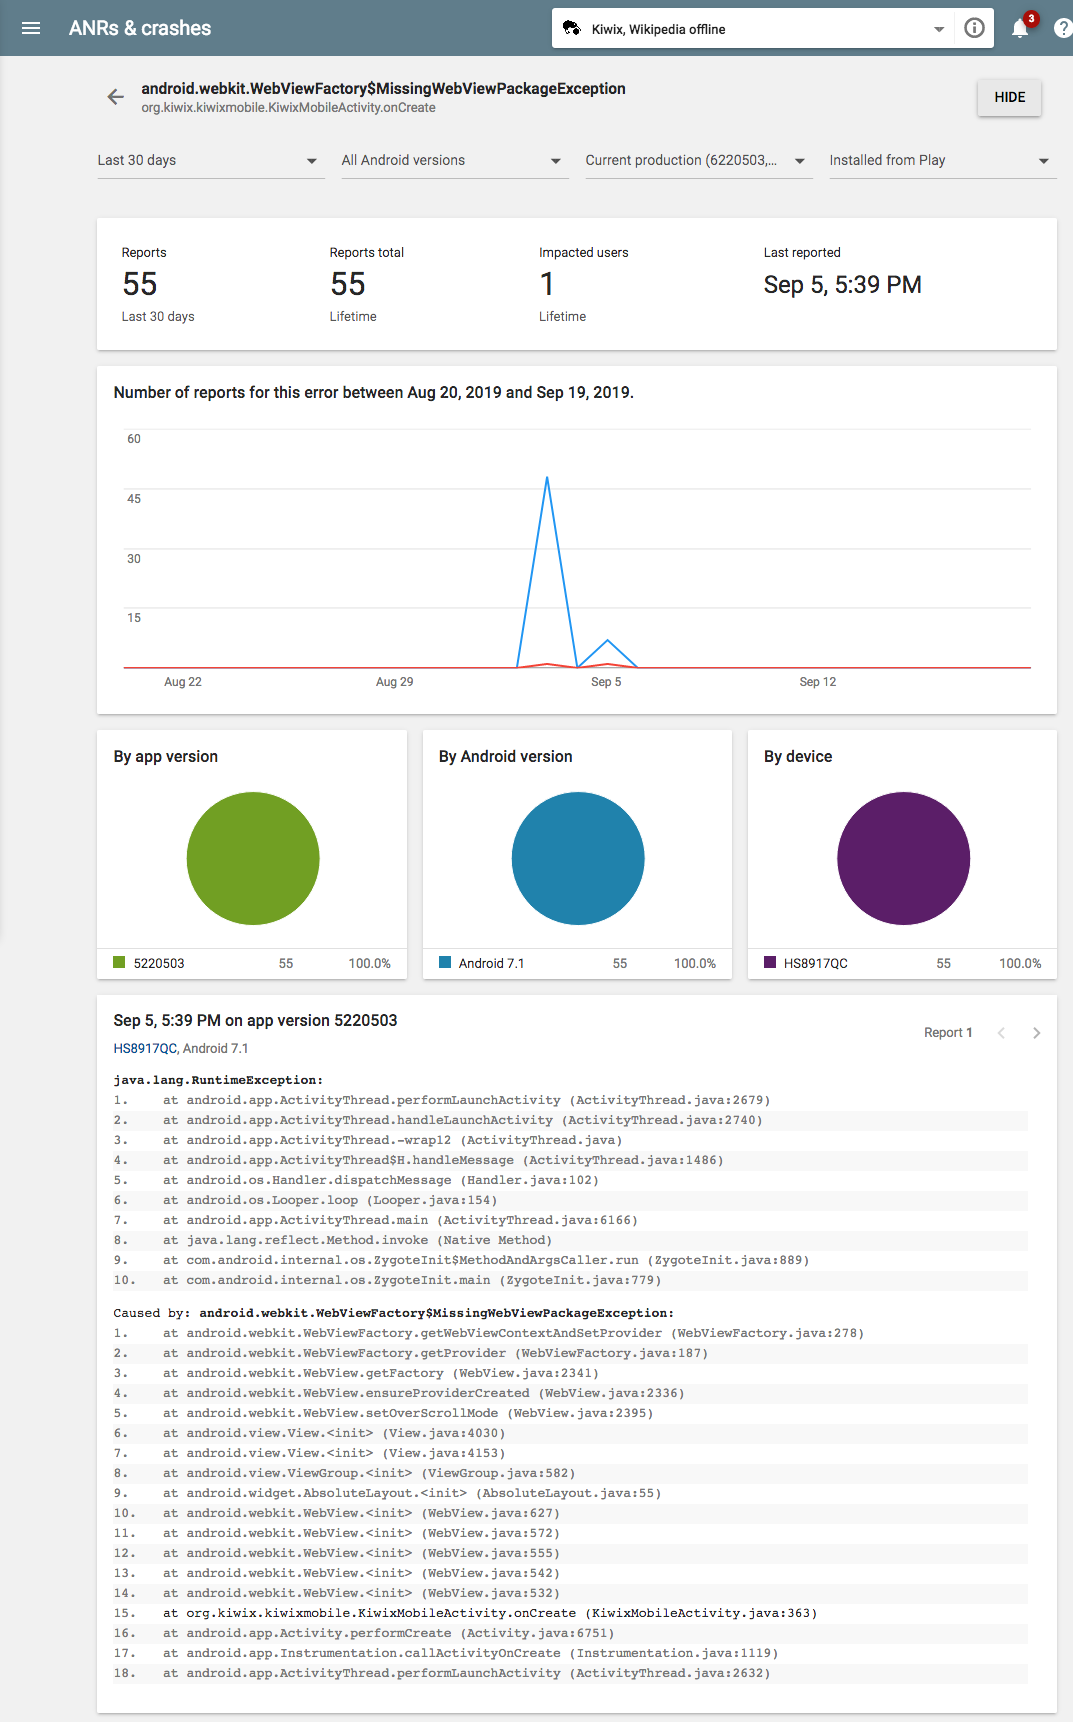
\includegraphics[width=13.5cm]{images/android-vitals-screenshots/55-crashes-WebViewFactory-MissingWebViewPackageException_2019-09-19-kiwix_trimmed.png}
    \caption{Kiwix Android 55 crashes for one user}
    \label{fig:55-crashes-WebViewFactory-MissingWebViewPackageException}
\end{figure}

\FloatBarrier

\subsection{Outcomes}
\textit{(Describe the outcomes resulting from the intervention). Not the speculative analysis, here it’s the concrete analysis of what was done.}

%\akb{The unsuccessful mini experiments make it hard to pick out which of the analytics related actions contributed to the first outcome reported below}

This case study led to several distinct forms of outcomes. The first was the dramatic improvement in the crash rate of the experiment app - Kiwix. The second was the development and adoption of opensource software - Vitals Scraper - which facilitated the collection and retention of otherwise ephemeral analytics information. And the third was the collaboration with the engineering team for Google Play Console as we discovered and reported various flaws in Google Play Console and Android Vitals. 

The mini-case studies did not provide direct outcomes (as neither provided the intended results). Instead they provided a couple of indicators that inform ongoing engineering practices and research. The first indicator, is that some failures may be impractical to reproduce within the time and other resources available at the time to the development team. Analytics tools such that measure [un-] reliability may help those teams measure the effects of their changes once the release is being used. The second indicator is that even promising research tools may also be impractical to apply beyond the immediate ecosystem that created that tool or after that research was published. The group that created CrashScope also provided a running instance of it at the time, however the service has not functioned on demand and the underlying software isn't available for others to use. Opensourcing the code of such tools provides an incomplete approach to enabling others to use and reuse the work. The code needs to include adequate support and ideally be maintained on an ongoing basis, something that seldom occurs for a multitude of reasons.

%%%% Table generated originally by Spread-LaTeX
%\begin{adjustwidth}{-1 cm}{-1 cm}
\begin{threeparttable}[!htp]\centering
\caption{Reductions in Crash Rates}\label{tab:kiwix-evaluation-reductions-in-crash-rates}
\scriptsize
\begin{tabularx}\textwidth{llrr} % SHOULD-DO I'd like to reduce the width slightly.
\toprule
%& & & & \\
&\multicolumn{3}{c}{30-day crash rates reported in Android Vitals~\tnote{0}} \\
\midrule
\multirow{2}{*}{.} &\multicolumn{2}{c}{Kiwix Apps} \\
Stage &Release&\cellcolor[HTML]{efefef}Experiment &Control  \\

&\cellcolor[HTML]{efefef}&\cellcolor[HTML]{efefef}Kiwix & WikiMed English \\

1 &0 
  &\cellcolor[HTML]{efefef}5.07\% &1.13\% \\
2 &1 &\cellcolor[HTML]{efefef}3.12\%~\tnote{1} &\multirow{2}{*}{\cellcolor[HTML]{A8A8A8}}... \\
3 &2~\tnote{2} &\cellcolor[HTML]{efefef}1.59\%~\tnote{3} & \cellcolor[HTML]{A8A8A8}... \\
  &3 &\cellcolor[HTML]{efefef}0.53\%~\tnote{4} &1.09\%~\tnote{5} \\
4 &4 &\cellcolor[HTML]{efefef}0.72\%~\tnote{6} &0.60\%~\tnote{7} \\
  &4~\tnote{8} 
&\cellcolor[HTML]{efefef}0.55\% &0.41\% \\
  &5 &\cellcolor[HTML]{efefef}0.40\%~\tnote{9} &0.26\%~\tnote{10} \\
\bottomrule
\end{tabularx}
\begin{tablenotes}
  \item[0] Except when otherwise noted.
  \item[1] Kiwix Release 2.5 with the previous custom download facility replaced by a Google Android downloader.
  \item[2] The code is under 25 lines including 10 lines of comments~\url{https://github.com/kiwix/kiwix-android/pull/1388}.
  \item[3] Aggregate crash rate over 7 days for versions 2.4, 2.5.1, 2.5.2, 2.5.3 (to Aug \nth{26} 2019).
  \item[4] Previous 30 days crash rate, before release 3.1.2 pushed the crash rate up (same graph as TODO).
  \item[5] \emph{Unchanged release from the first control.}
  \item[6] Includes 3.1.2 which had an average (mean) crash rate of roughly 1.7\% (roughly \nth{31} Dec 2019).
  \item[7] A mixed set of crash rates, averaged by Android Vitals. For the first updated release of Wikimed (the 2019-12 release).
  \item[8] As usage increased of the more reliable releases the averages declined.
  \item[9] The crash rates for releases 3.2.1 are 0.23\% and 3.3.1 are 0.31\%
  \item[10] Release 2020-03 actually has a crash rate of around 0.05\% the numbers are higher as there are still significant volumes of usage on the previous 2 releases.

\end{tablenotes}
\end{threeparttable}
%\end{adjustwidth}
\vspace{5mm}
%%%% Isabel recommends creating a timeline instead - sounds good SHOULD-DO

Table~\ref{tab:kiwix-evaluation-reductions-in-crash-rates} provides a comparison of the crash rates for the experiment and the control apps over four stages of this case study. There were three phases that interleave with these four stages.

The stages are:
\begin{enumerate}
    \itemsep0em
    \item The baseline,
    \item Simplifying the most buggy code (which was the downloader),
    \item Applying the concepts in the research to the experiment,
    \item The new normal.
\end{enumerate}
% Great ideas to reduce space in list items in https://tex.stackexchange.com/questions/6081/reduce-space-between-enumerated-items
% COULD-DO I've only applied the basic suggestion for this single list so far, might be worth thesis wide changes as the thesis matures.

The active part of the experiment started in stage 3 of this case study, although the initial research into the feasibility started several months earlier during the baseline stage.

\subsection{Stage 1: the baseline}
Before the experiment started there was little focus on finding and fixing causes of crashes. The development team did fix some sporadically, however they seldom used the reports from Android Vitals to identify crashes or address them.

The core app included an integrated download facility to download content to a user's local device. Files sizes ranged from a few MB to over 60GB and could take several days to download, especially in areas where connectivity wasn't ideal.  This integrated download facility provided users with several useful features, for example, they could pause and restart downloads. It also had an integrated recovery mechanism to restart and continue partial downloads after a failure, and it provided users with a progress indicator. However, this custom download facility had numerous bugs and was the largest source of crashes in real world use.

The custom apps were pre-packaged with content (which Google Play Services downloaded at the same time as downloading the app's binary). They did not need, and did not include the custom downloader. This meant their crash rates were significantly better (lower) than the core app managed.

\subsection{Stage 2: simplifying the most buggy code}
The first release, release 1 in the table, predated the hackathon (which was the start of the experiment). In this release the lead developer decided to replace a large body of custom code with generic downloader code rather than focus on fixing individual sections of code~\footnote{The combined commit with this change is~\href{https://github.com/kiwix/kiwix-android/commit/fcac33cf2daed5cea98387743c5c5dc52d59e09a}{commit fcac33cf2daed5cea98387743c5c5dc52d59e09a}}. The custom code was considered too problematic to fix. However, there was a trade-off by increasing the reliability there was a reduction in usability and also an impact on what happened when downloads stopped or otherwise failed before completion. The crash rate reduced to under 2\% once most users had the release with the new downloader installed.

\subsection{Stage 3: applying the research concepts of the experiment app}
I convinced the the leaders of the Kiwix project that we might be able to reduce the crash rate significantly by applying the concepts described in chapter 5. They had slowly become increasingly aware of the excessively high crash rate and the potential impact on both users and the app store's ranking of the apps based on the high crash rates. 

We agreed we would start by focusing on several of the most frequently occurring crashes as reported in Android Vitals. The opportunity to do so was at a week-long hackathon in Stockholm in August 2019. I led the discussions and analysis with several of the volunteer developers at the hackathon.

Following this discussion and analysis about the crashes being reported in Android Vitals for version \texttt{2.5.0} of the core application, the developers fixed several of the causes of the most frequent crashes with a surprisingly small amount of code of under 25 lines (including 10 lines of text added to the release log)\footnote{\url{https://github.com/kiwix/kiwix-android/pull/1388}}. Of interest, at least one of the fixes had actually been made and committed to a pending major release of the app but wasn't applied to the current production release~\emph{until the effects of the crash was made visible using analytics}. Details of the crash report and fix are available online~\url{https://github.com/kiwix/kiwix-android/issues/1261}~\footnote{The release was rolled out in Google Play to end users in stages from \nth{19} to \nth{23} August 2019 in stages, through an overabundance of caution given the small footprint and nature of the changes.}. The crash rate stabilised around 1.1\% once the majority of userbase had release 2.5.3 installed; it would have been lower were it not for the \texttt{UnsatisfiedLinkError} exceptions, discussed next.

Several new crash clusters emerged for \texttt{UnsatisfiedLinkError} exceptions. These were not directly related to the crash fixes in the \texttt{2.5.x} releases, instead they were related to the project choosing to apply advice from Google to use App Bundles~\citep{android_app_bundle}~\footnote{In practice, app releases often include a mix of bug fixes together with other changes so it is sometimes impractical to measure the effects of bug fixes in isolation. Similar challenges and behaviours exist in code commits,~\citep{partachi2020_flexme_untangling_commits} discusses that topic well. Nonetheless approaches used to detangle commits are unlikely to work as-is for releases as releases need to satisfy other constraints. Release planning and release management are discussed in~\href{chapter-related-work}{\nameref{chapter-related-work}}}.
%
With App Bundles Google Play took responsibility for delivering the correct app binaries to suit the end-user's device's hardware architecture~\emph{e.g.} ARM 32-bit, ARM-64 bit, Intel 64-bit, and so on. However, sometimes the users seemed to receive one or more binaries that didn't run on their device which led to this crash. What wasn't well published is enabling App Bundles is similar to Caesar crossing the Rubicon~\footnote{\url{https://grammarist.com/idiom/cross-the-rubicon/}} - there's no turning back. Therefore, rather than having the option to revert to `fat binaries' the project had to find an approach that worked in the context of App Bundles. As the Kiwix Android apps include a native library, written in C++, the solution needed to work for native code in addition to managed code.

There's quite a detailed issue report available on GitHub.com,~\href{https://github.com/kiwix/kiwix-android/issues/1259}{Issue 1259 - Crash Report: \texttt{UnsatisfiedLinkError} reported in Android Vitals for 2.5.x users}. The cause required in-depth investigation, changes to the build process, and changes to the application code in order to reduce the likelihood of the incorrect binaries being deployed to the end user devices.

Various developers continued to make corrective changes to the codebase which made ongoing incremental improvements to the app released to the \texttt{2.5.x} releases.

\subsection{Stage 4: the new normal}
The improvements in the reliability of the core app were sufficiently compelling \emph{and} the reliability of the custom apps sufficiently poor that the development team chose to refresh the majority of the custom apps, including the one used as the control (WikiMed English). Note: Various details of the crash rate at the time and the plan to migrate the custom apps are included in~\url{https://github.com/kiwix/kiwix-android/issues/1426}. 

All the apps share a common codebase, they are created using a common set of build scripts, they differ in their data contents, various `resources'~\footnote{\emph{``Resources are the additional files and static content that your code uses, such as bitmaps, layout definitions, user interface strings, animation instructions, and more."}~\url{https://developer.android.com/guide/topics/resources/providing-resources}}, and the custom apps exclude file management and download features as the contents are pre-packaged as part of the build process instead.

Several releases later, each with various changes and improvements aimed at fixing causes of crashes the crash rate was materially lower than when we started, at the time of writing the overall crash rate for the last 7 days is 0.54\% which is inflated because the rash rate for the previous release (\texttt{3.1.2}) spiked at 1.38\%, compared to 0.18\% for release (\texttt{3.0.5} -  the last production release) and 0.25\% for the recently released fix (\texttt{3.1.3}).



\subsubsection{Improvements in the crash rates}
Improvements in the crash rate came in three phases:
\begin{enumerate}
    \itemsep0em
    \item Replacing the custom downloader with core Android functionality in version 2.5 of the Kiwix app.
    \item Targeted crash fixes found and addressed during a hackathon in Stockholm, Sweden.
    \item Ongoing crash fixes, combined with migration of code from Java to Kotlin.
\end{enumerate}

\textbf{Phase 1}: As reported here and in \cite{harty_google_play_console_insightful_development_using_android_vitals_and_pre_launch_reports} and \cite{harty_better_android_apps_using_android_vitals} the Kiwix Android app had a very high overall crash rate caused by several significant flaws in the app. The project team released version 2.5 of the main Kiwix app in July 2019. As figure \ref{fig:kiwix_crash_rate_drops_v2_5} shows, the crash rate decreased significantly as version 2.5 rolled out to the majority of the userbase. %In the last 30 days the crash rate was 1.87\% down from 5.07\% in February 2019.

One of the major changes in version 2.5 was the replacement of the in-house download utility with the default Android Download Manager\cite{kiwix_release_2_5_0}. The in-house, custom, version was a major source of crashes, and the replacement obviated a class of crashes, however it did so at a price in terms of functionality and usability. The in-house download utility allowed users to pause and resume downloads, and it would complete failed partial downloads. Users also received updates on the progress of the downloads, important when they often took many minutes or even hours or days in some cases (such as for multi-GB downloads over poor, slow, unreliable connections on low-end devices).

\begin{figure}[htbp!]
    \centering
    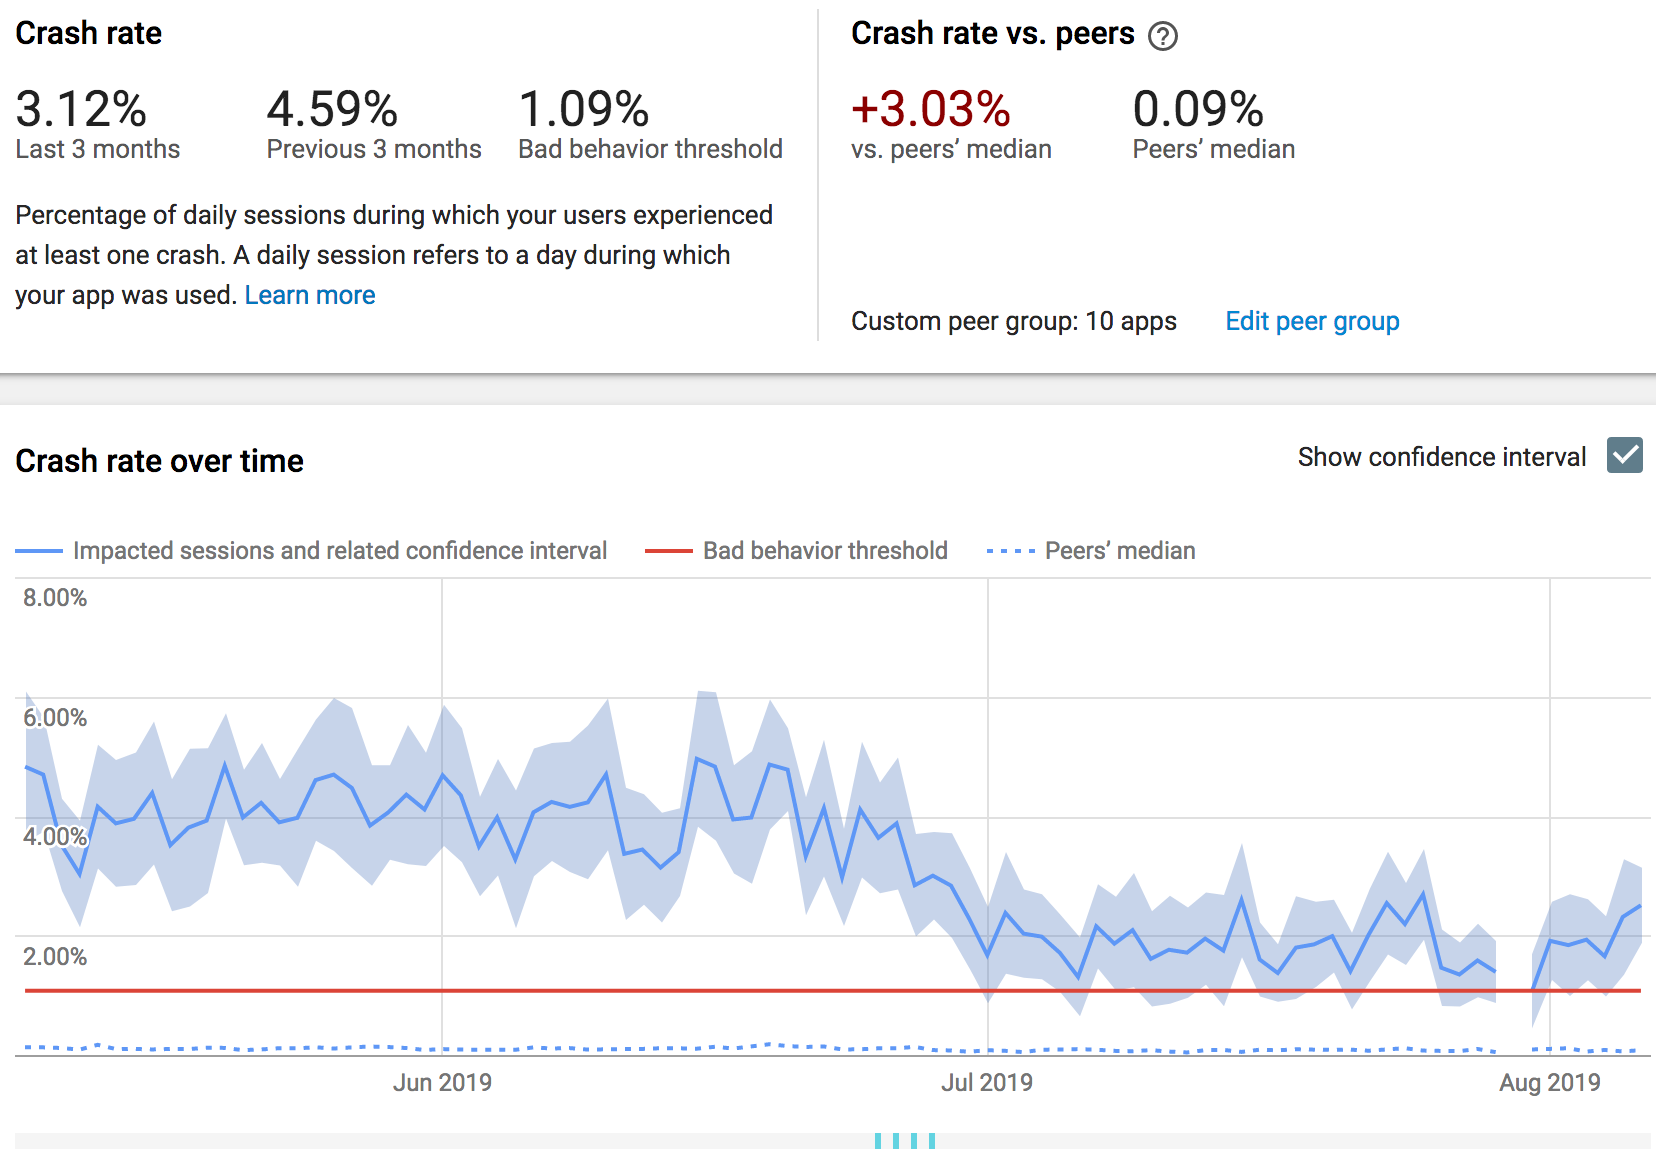
\includegraphics[width=\textwidth]{images/android-vitals-screenshots/kiwix-crash-rate-drops-with-v2_5.png}
    \caption{Kiwix Crash Rate Drops with V2.5 Release}
    \label{fig:kiwix_crash_rate_drops_v2_5}
\end{figure}

\textbf{Phase 2}: Following initial discussions about the crashes being reported in Android Vitals for version 2.5.0 of the Kiwix application, a group of the developers for the Kiwix projects collaborated on a week-long hackathon in Stockholm in August 2019. One of the areas the developers worked on was to focus on identifying and addressing some of the biggest contributors to the high crash rate. 
%

%%%%% Consider whether to convert the following two visual figures to code listings so they can be included in the Code Listings in the table of contents. 
\begin{figure}
    \centering
    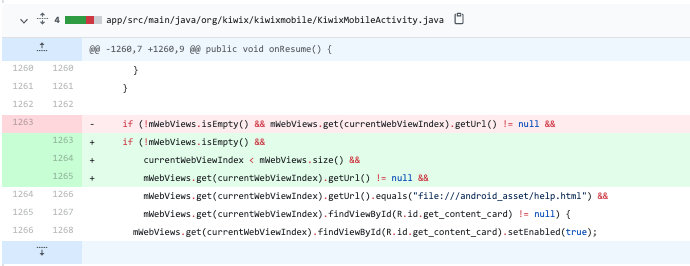
\includegraphics[width=14cm]{images/github/kiwix-pr1388-extract-1.png}
    \caption{First material change in PR-1388 for Kiwix Android}
    \label{fig:kiwix_pr1388_extract_1}
\end{figure}


\begin{figure}
    \centering
    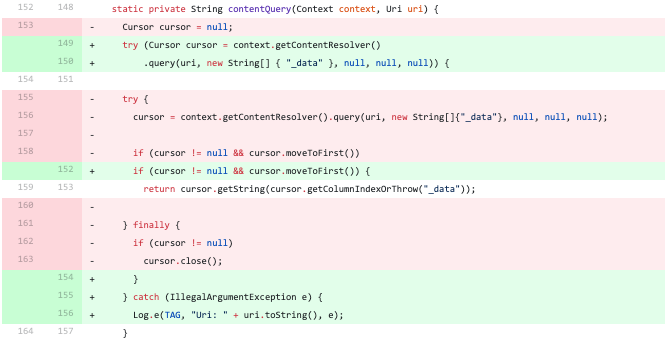
\includegraphics[width=14cm]{images/github/kiwix-pr1388-extract-2.png}
    \caption{Second material change in PR-1388 for Kiwix Android}
    \label{fig:kiwix_pr1388_extract_2}
\end{figure}


The developers ended up fixing some of the causes of the most frequent crashes with a surprisingly small amount of code of under 25 lines (including 10 lines of text added to the release log)\footnote{\url{https://github.com/kiwix/kiwix-android/pull/1388}}. Figures~\ref{fig:kiwix_pr1388_extract_1} and~\ref{fig:kiwix_pr1388_extract_2} illustrate the material changes that were made to address two of the crashes. The first adds another null check: \small{\texttt{currentWebViewIndex < mWebViews.size() \&\&}}. 
The second catches an \texttt{IllegalArgumentException} if one occurs. 

According to Android Vitals, the crash rate was more than halved once release 2.5.3 had rolled out to the majority of the userbase, for example for the 30-day period of \nth{19} Aug 2019 to \nth{16} Sep 2019 the overall crash rate was 1.47\% for the Kiwix app. Figure~\ref{fig:kiwix_android_vitals_with_gaps_2019_09_20} is the source of this data. Several aspects of this figure will be discussed in more detail in the \href{section-flaws-in-the-analytics}{\nameref{section-flaws-in-the-analytics}} topic. For now, the main point to highlight in this figure is the difference between the crash rates for two different builds of the 2.5.3 release, 0.96\% for 6220503 versus 2.22\% for 5220503. These builds were for different hardware architectures of Android where crashes related to Android App Bundles occurred more often for the 5220503 release. Further analysis of these crashes are in the~\href{kiwix-android-app-bundling-crashes}{\nameref{kiwix-android-app-bundling-crashes}} topic.

\begin{figure}
    \centering
    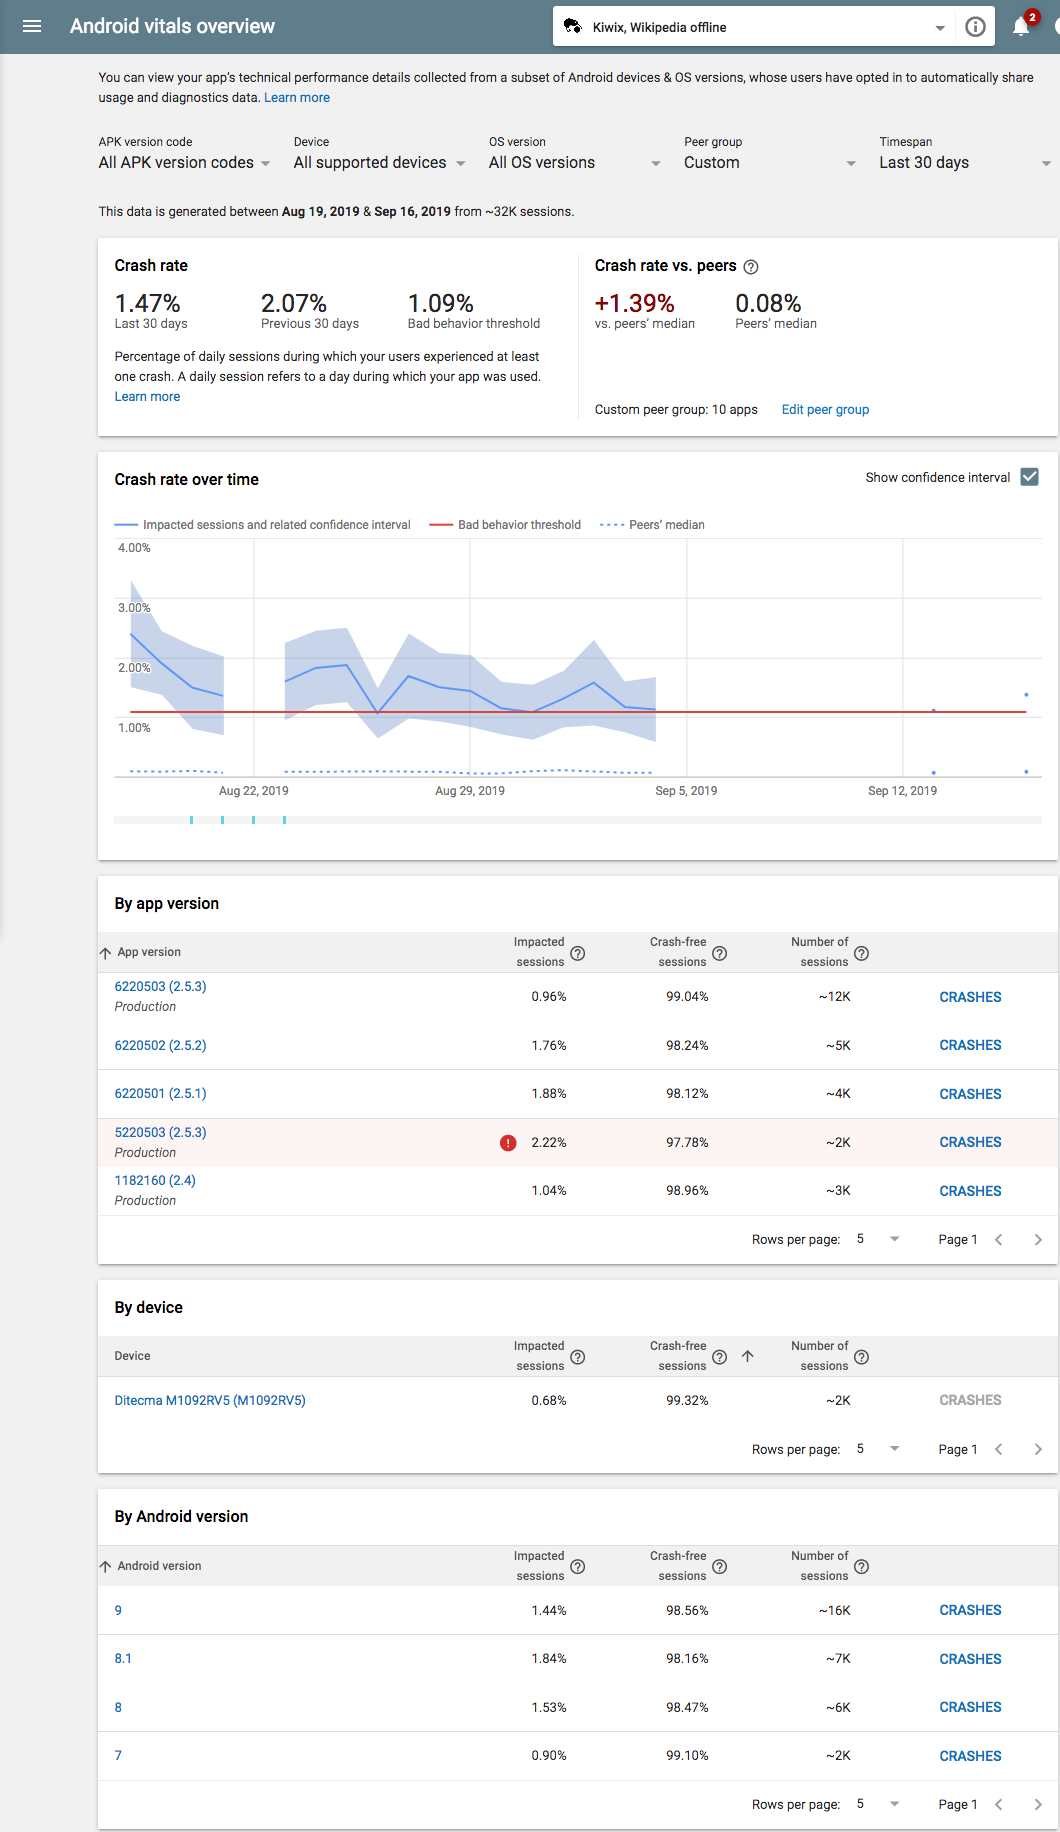
\includegraphics[width=12.5cm]{images/android-vitals-screenshots/Screeenshot_2019_09_20_Android_Vitals_Overview_Kiwix_Google_Play_Console.png}
    \caption{Android Vitals overview for Kiwix, 30 day view on \nth{20} Sep 2019}
    \label{fig:kiwix_android_vitals_with_gaps_2019_09_20}
\end{figure}


Various developers continued to make corrective changes to the codebase which made ongoing incremental improvements to the app released to the \texttt{2.5.x} releases. 



\textbf{Phase 3}: Several developers for the Kiwix project, the lead developer in particular, have been actively reviewing crashes reported by Android Vitals, filing issues, and addressing the causes of the crashes in order to reduce the crash rate and improve the app's stability. For the Kiwix project crashes are tracked as issues on GitHub, on~\nth{11} June 2021 there are 182 closed and 8 open issues that mention `crash': 182 closed, 8 open % Was 133 closed, 6 open.
\footnote{\url{https://github.com/kiwix/kiwix-android/issues?q=is\%3Aissue+crash}}
%COULD-DO analyse each issue to identify the source of the crash.

Several releases later, each with various changes and improvements aimed at fixing causes of crashes the crash rate was materially lower than when we started, in early 2020 the overall crash rate for the last 7 days was 0.54\% which is inflated because the rash rate for the previous release (3.1.2) spiked at 1.38\%, compared to 0.18\% for release (3.0.5 -  the last production release) and 0.25\% for the recently released fix (3.1.3).


\textbf{A Quick discussion on perspectives and views}. 
One of the key challenges when trying to interpret Android Vitals analytics is to determine comparisons and to establish reference points. For instance, are the recent crashes related to the embedded WebView component related to changes in the app, in the Android platform, to a particular device manufacturer? 

For instance, the most frequent crash in the 60 days to \nth{11} Jun 2021 has only occurred on Huawei devices for the most recent release of the Kiwix app (3.4.4). The crash is:

\begin{lstlisting}
java.lang.IllegalStateException
org.kiwix.kiwixmobile.core.main.CoreReaderFragment.webViewFailedLoading
\end{lstlisting}

that affected 16 users a total of 96 times in these 60 days. % https://play.google.com/console/developers/9116215767541857492/app/4975184706939091905/vitals/crashes?errorType=CRASH&versionCode=6230404%2C5230404%2C4230404%2C3230404&days=60&installedFrom=PLAY_STORE
Could this be related to The US government's ban on Huawei including the prevention of Google software from being installed on new Huawei models?~\footnote{\url{https://www.cnet.com/news/huawei-ban-timeline-chinese-company-android-rival-coming-phones-tablets/}~\citep{androidauthority2021_the_huawei_ban}, \url{https://www.androidauthority.com/huawei-google-android-ban-988382/}} and/or the Android WebView component being disabled, or yet another as yet unknown cause? (For instance perhaps it's a similar crash to the one reported on some models of Samsung S9 and S9+ phones~\citep{ebling2018_so_s9_specific_webview_device_crash_report}? Understanding the reasons may help the developer decide on a suitable method to address the runtime failure in the app and/or provide a better user-experience.

% Some notes are in a the draft materials document in \href{section-experiments-with-webviews}{\nameref{section-experiments-with-webviews}}.



\subsubsection{Vitals Scraper}
~\href{section-vitals-scraper}{\emph{Vitals Scraper}} was developed to facilitate the collection, preservation, and sharing of reports and data presented in Google Play Console and Android Vitals. Details of the software's design and implementation are discussed in the~\href{chapter-code-needed}{\nameref{chapter-code-needed}} chapter.

\begin{figure}
    \centering
    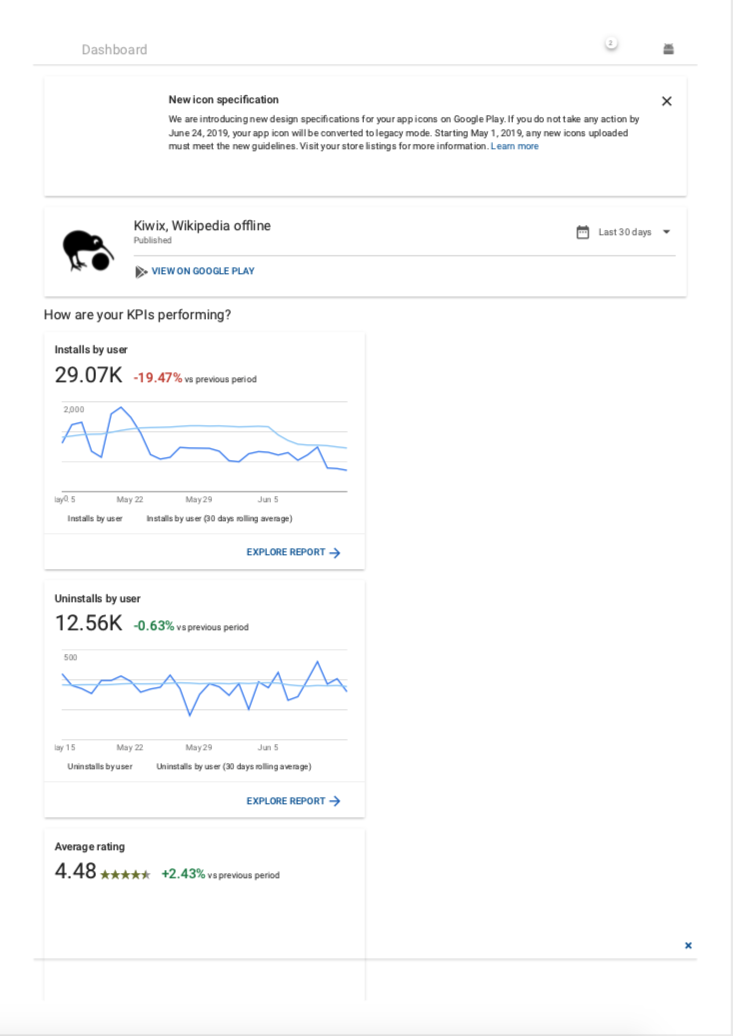
\includegraphics[width=7cm]{images/google-play-console/Dashboard - Kiwix-Google-Play-Console-(2019-Jun-14)-p1.png}
    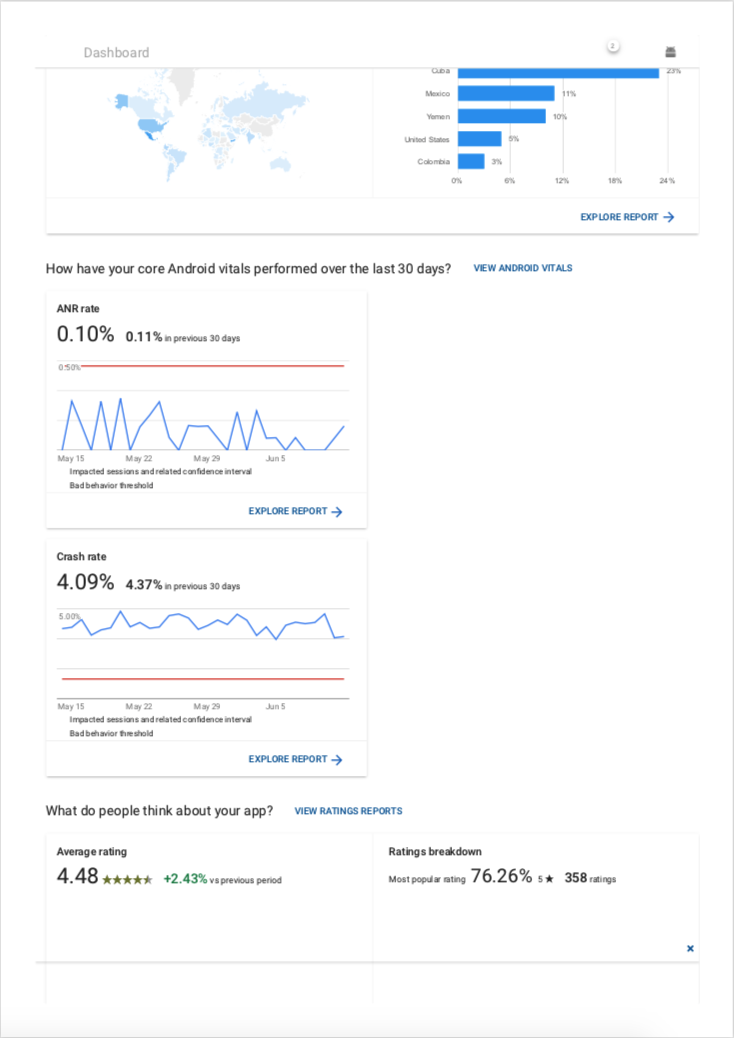
\includegraphics[width=7cm]{images/google-play-console/Dashboard - Kiwix-Google-Play-Console-(2019-Jun-14)-p3.png}
    \newline
    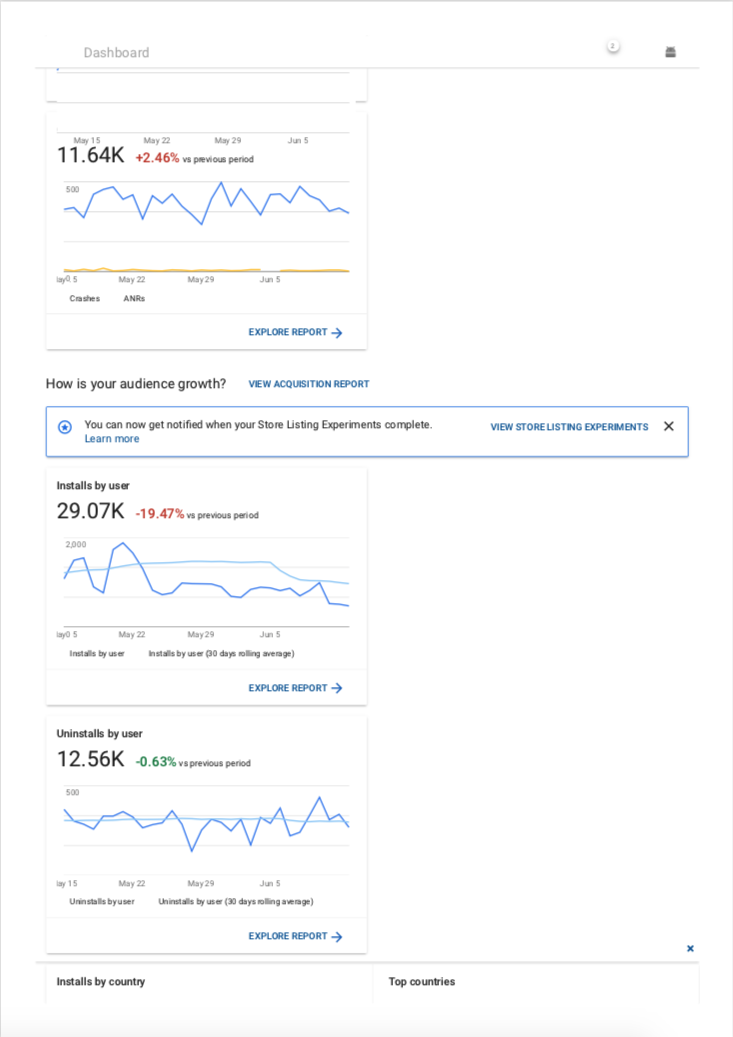
\includegraphics[width=7cm]{images/google-play-console/Dashboard - Kiwix-Google-Play-Console-(2019-Jun-14)-p2.png}
    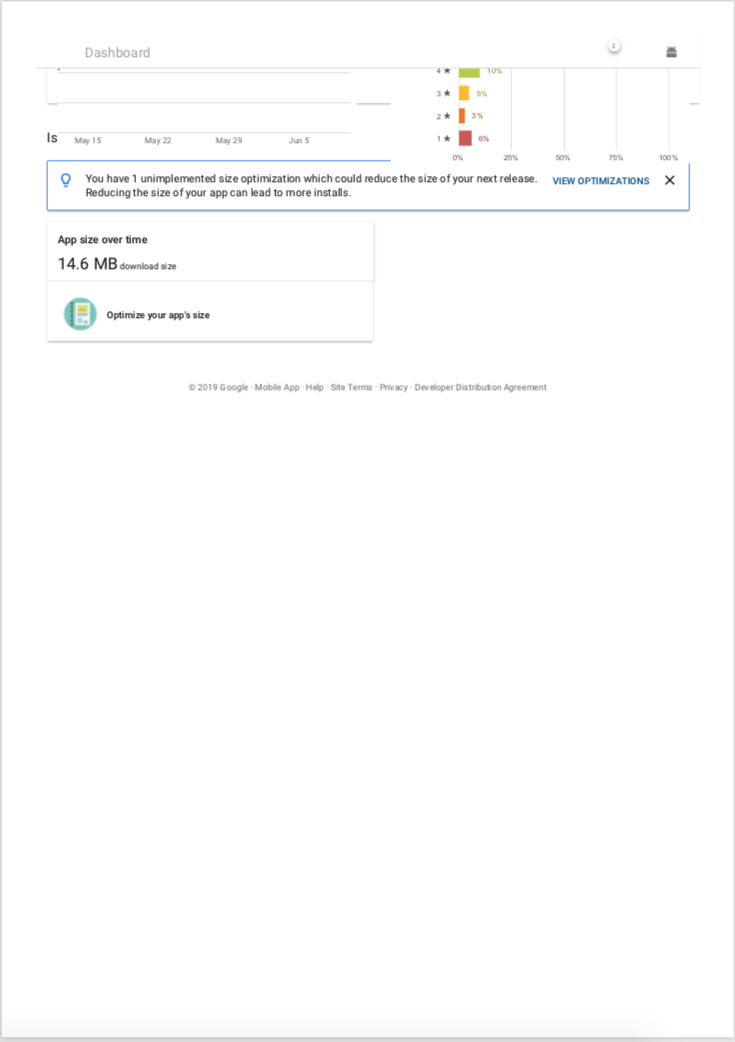
\includegraphics[width=7cm]{images/google-play-console/Dashboard - Kiwix-Google-Play-Console-(2019-Jun-14)-p4.png}
    \caption{Print web page of Dashboard in Google Play Console}
    \label{fig:screenshot-dashboard-gpc-kiwix}
\end{figure}

To help illustrate why tools such as Vitals Scraper was developed, Figure~\ref{fig:screenshot-dashboard-gpc-kiwix}, shows the results of printing the dashboard for the Kiwix app in Google Play Console on \nth{14} June 2019, in order to record the analytics reports for the app. Content is poorly formatted and split across pages, and web page pop-ups sometimes overlaid and obscured the contents of the report. (Some of the flaws illustrated in the contents of the report will be discussed shortly).

Vitals Scraper was able to extract data from various on-screen reports that wasn't otherwise available. It also generated cleaner reports saved as images. Vitals Scraper was jointly developed with Joseph Reeve as an opensource project and tested independently by a lead developer of one of the commercial app projects mentioned later in this thesis as part of evaluating the applicability and generality of the software. It could be scripted and run unattended to facilitate data collection at scale and as an ongoing basis.

In terms of this research, Vitals Scraper was used to collect analytics reports for multiple projects and development teams including the Kiwix apps. 


\subsubsection{Flaws in the analytics}~\label{section-flaws-in-the-analytics}
Various flaws and/or limitations were discovered in the analytics through using them. Their discovery led eventually to collaborating with the relevant engineering team at Google who were responsible for the analytics and for Google Play Console, which is discussed in the next topic.

You may already have noticed that the previous two figures both contain visible flaws. Figure~\ref{fig:kiwix_crash_rate_drops_v2_5} has a gap in the graph, and figure~\ref{fig:screenshot-dashboard-gpc-kiwix} already illustrates at least one flaw, where two reports (the installs by user and uninstalls by user) were repeated in the dashboard for the Kiwix application (on the first and second pages of the print out). 

Fourteen of the flaws were published in a poster that supported my short paper at MOBILESoft 2020~\citep{harty_improving_app_quality_despite_flawed_mobile_analytics}. The flaws discovered in Google Play Console and Android Vitals are also itemised in Table~\ref{tab:issues-in-google-play-console-reports} in the discussion chapter which combines flaws from several case studies.

A key consideration is to determine if they were local in scope or more general. They were cross-checked in several dimensions:
\begin{itemize}
    \item Across apps on the same Google Play Console account.
    \item Across multiple Google Play Console accounts.
    \item For other logins.
    \item With the engineering team who created and provided the analytics service. 
\end{itemize}

All of these checks eventually use the same source of analytics data - that gathered by Google Play Services running on end-user Android devices~\footnote{More precisely, by design, the data is collected from Android devices where the device manufacturers have satisfied Google's requirements where those devices have various Google software pre-installed. There ~\emph{may} be additional sources of the data e.g. where Google Apps have been installed subsequently using GApps~\citep{opengapps} or similar services including~\citep{nikgapps}.}.
%
Subsequent case studies extend the comparisons to additional sources of analytics for similar analytics events, particularly crashes.

As some flaws are data dependent sometimes they cannot be checked for every app and every login for every period. On this basis there may be other flaws that I did not experience.

When several of the flaws emerged they were reported to Google through two channels. The first is available to Android developers when they are using Google Play Console, through a feedback menu option in the Google Play Console user interface. The second was through directly contacting a public member of the product team for Google Play Console and Android Vitals, at that time Fergus Hurley. 

\begin{comment}
The bugs include inconsistencies in the crash rate, reported variously as 6.75\%, 5.48\%, and 5.07\% for the main Kiwix app. The values are found in various sections of the data, however, it's not clear why each is favored in particular areas of the Reports.

\nth{14} March 2019
FYI I've also found the counts of Crashes (11.99K) https://play.google.com/apps/publish/?account=9116215767541857492#AppDashboardPlace:p=org.kiwix.kiwixmobile&appid=4975184706939091905  is higher than either the last 30 days of crashes and even the combination of crashes and ANRs (assuming my copy+paste and manual editing didn't lose any data). https://play.google.com/apps/publish/?account=9116215767541857492#StatisticsPlace:p=org.kiwix.kiwixmobile&appid=4975184706939091905&statms=DAILY_ANDROID_METRICS_CRASHES&statms=DAILY_ANDROID_METRICS_ANRS&statg=DAILY&ts=THIRTY_DAYS I've attached the calculations in an Excel spreadsheet so you can check these if you wish.

I've made quite a few changes, partly after a good discussion today with Fergus Hurley at Google who challenged lots of details in the flaws section and wanted as much feedback and suggestions as possible on ways I'd like the tools improved.
\end{comment}

\begin{comment}
Issues reported using Google Play Developer Support on \nth{19} June 2018, Google replied on \nth{19} July 2018, one month later (many times longer than their published response time of a few days at the time).

Please see a copy of your initial inquiry:

"The pre-launch reports indicate the tests aren't actually running these 
days. Instead it states the app is incompatible with all 14 devices with 
the following error message: "Devices incompatible with APK" 

And I had asked for these two items in response:
Which APK version code you wish to view the pre-launch report for?
Screenshot of the page you're viewing(these are really helpful!)

\nth{24} July 2018: 
 I'm still seeing some test runs in the pre-launch report that claim some devices aren't compatible, and also many more test runs that don't seem to run any tests at all. 

It's not obvious why sometimes the number of devices varies - do you have any idea why? e.g. sometimes the tests seem to be scheduled on 9 devices, other times 7, and often 0

I've attached a couple of screenshots.
And here's a URL for the test run with 7 devices
https://play.google.com/apps/publish/?account=9116215767541857492#PreLaunchReportPlace:p=org.kiwix.kiwixmobile&plrtab=CRASH&plrvc=1181980
and here with 9 
https://play.google.com/apps/publish/?account=9116215767541857492#PreLaunchReportPlace:p=org.kiwix.kiwixmobile&plrtab=SCREENSHOTS&plrvc=181980

Also, in case you're interested, the Pixel 2 device sometimes reports an extremely long start up e.g. 16K (presumably milliseconds) as shown in one of the attached screenshots however, watching the video it's clear the tests are interacting with the app and the app is responding within a couple of seconds. This quirk seems to happen mainly on the Pixel 2 - perhaps there's a bug in how it (the device model) reports activity? Any suggestions?

And sorry I realise I didn't provide an example of where the pre-launch report claims the devices/the app are incompatible. Here you go, a screen shot and here's the URL
https://play.google.com/apps/publish/?account=9116215767541857492#PreLaunchReportPlace:p=org.kiwix.kiwixmobile&plrvc=4181770&plrtab=SCREENSHOTS
This is from 26th June, there were only 1 set of reports, all on 26th June so I'm presuming we tried to push one release, probably with various platform-specific APKs.

Thanks for your reply and detailed notes, screenshots. Really helps us investigate! 

For the varying number of compatible devices on each APK upload, I checked in with our team and it seems they may vary from time to time. If you're noticing, especially that all devices show as completely incompatible and no tests are run, you may want to upload a new APK to try.

Secondly, thanks for reporting the behavior on the long startup time. I’ve documented this and escalated to our technical team for further investigation. Our team is working to resolve this issue for you as soon as possible.

I appreciate your patience and I’ll let you know the moment I have an update. 

Also I'd appreciate whatever you can discover about why the set of devices varies from one test run to another. e.g. is it random, based on load, or availability, or something hard to guess like the day of the week multiplied by the current temperature in NYC?

I understand your point. I’ll be sure to pass along your specific feedback to our product team on showing the reason for incompatibility. We’re continually adding new features and functionality, so please stay tuned.

For your second question, the help center mentions the following, and sadly I am not able to provide further information than this: 
Test devices are selected based on a wide range of criteria, including popularity, crash frequency, screen resolutions, manufacturers, operating systems, and more. The selection of test devices may vary. 
For your reference, there is a custom test functionality which gives you the ability to choose the device types and testing method. If you’d like to create a custom test using Firebase Test Lab for Android, at the top of your screen, you’ll see a “Run Custom Tests” banner if you're able to run a custom test. To begin, select Get Started. You can learn more about this feature in the Firebase documentation.

All the above was forwarded to Fergus who confirmed he'd forwarded the issues to the relevant team (March 2019).
\end{comment}

\begin{comment}
My email to Nick Fortescue (Googler on SO)

Started with \url{https://stackoverflow.com/questions/54519393/the-number-of-downloads-in-firebase-is-30x-different-from-the-google-console}
"The project has some thorny problems, particularly related to lifecycle bugs and our crash rate according to the Dev Console is around 5\%. I'm working with Fergus to see how we can improve the app and Android Vitals"
\end{comment}

\subsubsection{Collaboration with Google}~\label{section-collaboration-with-google}
In February 2019 I was reintroduced to the Engineering Director at Google Play and the head of the Google Play Console engineering team, Milena Nikolic, by a work colleague on a recent professional engagement who thought Google may be interested in my research and findings related to Google Play Console. After an in-person discussion about my research and findings she introduced me to Fergus Hurley who was the Product Manager for Android Vitals at the time. He took an active interest in my research, including reviewing and cross-checking various details of flaws in Android Vitals and Google Play I had discovered and reported to Google. 

One of the other case studies in particular, with the Catrobat project, overlapped this case study on the Kiwix project. The Collaboration with Google expanded in both depth and breadth as the analytics used by that project (Fabric Crashlytics in addition to Google Play Console and Android Vitals) provided additional vantage points and additional flaws surfaced through the collective analytics being used across the case studies. 

Google then introduced me to several senior members of the engineering team for Google Play Console and Android Vitals and requested a comprehensive report on the flaws and issues found through my research. This report was written and shared with them, it is based on a subset of the information and results presented in this thesis (which includes more recent updates and results from additional case studies). The team stated they do not acknowledge contributions, nonetheless they have ended up addressing some of the flaws and some of the requests for improvements to Google Play Console and Android Vitals. Hopefully the report and the collaboration had some postive influence, yet I'm aware of the rick of falling into the \textit{post hoc fallacy}~\citep{wikipedia_post_hoc_fallacy}, and illustrated in Figure~\ref{fig:xkcd-correlation}.

\begin{figure}
    \centering
    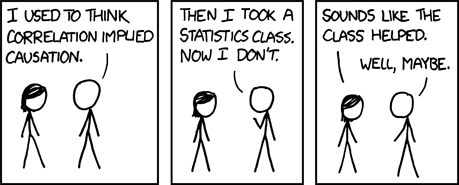
\includegraphics{images/xkcd/correlation-552.png}
    \caption{XKCD: Correlation, source \url{https://xkcd.com/552/}, used with permission.}
    \label{fig:xkcd-correlation}
\end{figure}

In terms of research hygiene, the research into the behaviours of Google Play Console and Android Vitals were debated and cross-checked with Google, and my paper~\citep{harty_google_play_console_insightful_development_using_android_vitals_and_pre_launch_reports} was reviewed by the Product Manager who was acknowledged with his permission in the paper.


\subsection{Discussion}~\label{case-study-kiwix-discussion}
\textit{(Explore what these outcomes mean for the use of analytics in mobile software more generally).}

Android Vitals is of limited value for low-volume apps as several reports are only available once there are data volumes to enable the data to be anonymized sufficiently to protect users' privacy. As the product owner confirmed at the time: \emph{``... it [information] only shows up for apps that have enough data to be privacy compliant"}~\footnote{unpublished correspondence with Google.}.

As reported in~\citep{harty_google_play_console_insightful_development_using_android_vitals_and_pre_launch_reports}, the Android Vitals reports were more relevant for apps with 10,000+ active users. Paradoxically, the threshold may be lower for apps which fail more often as they would generate more failure reports. However, actively testing this hypothesis may have adverse lifetime effects for the person who releases such poorly behaving apps, and knowingly doing so contravenes Google's policy for Google Play~\citep{google_play_developer_policy_center}~\footnote{The relevant section of the policy is currently available at:~\url{https://support.google.com/googleplay/android-developer/topic/9876964?hl=en&ref_topic=9858052,9857238,2856718,} and supported by training material at~\url{https://playacademy.exceedlms.com/student/path/65190-comply-with-google-play-s-spam-and-minimum-functionality-policies}}.


\textbf{MUST-DO} describe about the flaws discovered in GPC and Android Vitals and the discussions with Google Engineering.

\begin{comment}
Links to docs:
Android Developer Documentation: https://developer.android.com/topic/performance/vitals
Play Console Help Center: https://support.google.com/googleplay/android-developer/answer/7385505?hl=en-GB
Overview video: https://www.youtube.com/watch?v=vj3Y8L5HLdg

 https://android-developers.googleblog.com/2018/12/wrapping-up-for-2018-with-google-play.html, https://android-developers.googleblog.com/2017/07/android-vitals-increase-engagement-and.html and https://developer.android.com/topic/performance/vitals/ 
\end{comment}

\subsection{Summary of Kiwix Android Case Study}
% Joe's notes this is not compelling and doesn't compare with the other case studies.
% Why Kiwix, what did I gain, similarities and contrasts, why include in the PhD.

This is a long term study, where I was embedded as part of the development team for a period of the case study. We demonstrated it was practical to use only external, platform, analytics and still able to be effective in reducing the crash rate. For projects that do not use in-app crash reporting the platform tools are sufficient to make material improvements \emph{when the team actively monitors and addresses the crashes reported in the platform level analytics}. The practices need to be applied on a long term basis; with the loss of the project lead who focused on addressing the runtime failures the failure rates are increasing. Entropy increases.
% c.f. working with tech debt which has similar behaviours

%\akb{Include point about long term engagement needing tools like Vitals Scraper to provide data that can be used analyse performance of the app over time?}

The user interface of Google Play Console and Android Vitals was interactive and Google had removed an earlier feature where historic crashes could be downloaded for further analysis which meant the user interface was ephemeral, reports could not be stored easily (and even printing the reports as PDF files or on paper didn't capture the contents well) the user interface required human input and navigation, and retaining information for historical and trend analyses was difficult. Vitals Scraper was developed to address facilitate my ongoing research of this and other projects and enabled data, reports, crashes and ANRs to be recorded in ways that enabled comparisons and analysis. 

The case study was very useful in terms of providing  control and experiment apps. It was also the first of the experiments that set the scene and the direction for further case-studies.

The analytics reported on both \href{glossary_jvm}{JVM} and native crashes (written in C++) where that code is external and shared with various projects. 

% Provided materials published in various of my papers
This case study also led to the discovery of various flaws in Google Play Console and Android Vitals which led to the meetings, discussions and writing the report for the Google Engineering team. They have improved their product iteratively - v2 still had some flaws v3 has addressed some of these and similarly reduced some of the operability headaches.




%%%%%%%%%%%%%%%%%%%%%%%%%%%%%%%%%%%%%%%%%%%%%%%%%%%%%%%%%%%%%%%%%%%%%%%%
\par\noindent\rule{\textwidth}{0.4pt}
~\textbf{Earlier material follows}






% Following initial discussions about the crashes being reported in Android Vitals for version 2.5.0 of the Kiwix application, we collaborated on a week-long hackathon in Stockholm in August 2019. There, the developers ended up fixing some of the causes of the most frequent crashes with a surprisingly small amount of code of under 25 lines (including 10 lines of text added to the release log)\footnote{\url{https://github.com/kiwix/kiwix-android/pull/1388}}.



\subsection{Examples of real-time crashes}
Each of these examples exemplifies at least one characteristic of the reports that are provided by Android Vitals in Google Play.

\subsubsection{EsxRenderBucket::AddUnbucketedEntries(...)}
This crash is one of the most frequent crashes reported in early October 2020 and has been occurring on an ongoing basis according to Android Vitals for the current release of the Chemistry \& Physics simulations app (release 2020-04). Through analysis of the reports this crash only affects one release of the app (release 5200950) and it does not occur on the other three releases (6200950, 4200950, 3200950). It occurs on multiple manufacturer's device models, and on Android 9.0, 8.1, and 8.0). 

This crash is a native crash and mainly occurs within the context of \texttt{/system/app/Chrome/Chrome.apk} \textit{the web browser app created by Google!} The Kiwix apps rely on an embedded web browser, which is generally Google's Chrome browser, to render (\emph{i.e.} display) the content to the user\footnote{It also appears for other variants of the Android Chrome browser on some devices e.g. \texttt{/data/app/com.android.chrome-bAmCl9DcPfmqf3oKL54Efg==/base.apk (offset 0xbe7000)} and also the Android WebView component~\texttt{/data/app/com.google.android.webview-9ShSu\_81V02zu4ENrAjvJA==/lib/arm/libwebviewchromium.so} (also created by Google).}.

\begin{listing}[H]
\caption{Crash Cluster: EsxRenderBucket::AddUnbucketedEntries} \label{code:crash_cluster_add_unbucketed_entries}
\tiny
\begin{minted}{cpp}
*** *** *** *** *** *** *** *** *** *** *** *** *** *** *** ***
pid: 0, tid: 0 >>> org.kiwix.kiwixcustomphet <<<

backtrace:
  #00  pc 00000000001535a0  /vendor/lib/egl/libGLESv2_adreno.so (EsxRenderBucket::AddUnbucketedEntries(EsxCmdBufType, unsigned int)+132)
  #01  pc 0000000000152b17  /vendor/lib/egl/libGLESv2_adreno.so (EsxRenderBucket::BucketRenderingCmds(EsxRenderBucketParams*)+740)
  #02  pc 0000000000186a6d  /vendor/lib/egl/libGLESv2_adreno.so (EsxContext::BucketRenderingCmds(int)+712)
  #03  pc 00000000000e6987  /vendor/lib/egl/libGLESv2_adreno.so (EsxContext::BindDrawFramebuffer(EsxFramebufferObject*)+178)
  #04  pc 00000000000b6a5d  /vendor/lib/egl/libGLESv2_adreno.so (EsxContext::GlBindFramebuffer(unsigned int, unsigned int)+332)
  #05  pc 0000000001b8c659  /system/app/Chrome/Chrome.apk (offset 0x80c000)
\end{minted}

\end{listing}

Of the 53 crash clusters reported over the last 60 days for all Android versions and version 5200950 of the app, installed from Google Play, 16 of the 53 crash clusters are for this crash.

Searching local logs, generated using the opensource software~\texttt{vitals-scraper} that we created as part of this research we can see the same crash cluster has occurred in some, not all, of the Kiwix applications. The command used to find the files that contain this crash cluster is:~\texttt{grep -c EsxRenderBucket::AddUnbucketedEntries * | sort -t ':' -k 2 -g}. This returns a list of the files, sorted by the number of matches for the string found in each of the files. Here are the entries with at least one match.

\begin{listing}[H]
\caption{Logs that include crash cluster: EsxRenderBucket::AddUnbucketedEntries} \label{code:vitals_scraper_logs_add_unbucketed_entries}
\footnotesize
\begin{minted}{text}

android-crash-clusters-org.kiwix.kiwixcustomphet_1572958874833.json:2
android-crash-clusters-org.kiwix.kiwixmobile_1599898794048.json:2
phet-1-day-android-crash-clusters_1569599996989.json:2
android-crash-clusters-org.kiwix.kiwixcustomphet_1572966654935.json:3
android-crash-clusters-org.kiwix.kiwixmobile_1577913956806.json:3
android-crash-clusters-org.kiwix.kiwixcustomphet_1574380641173.json:4
android-crash-clusters-org.kiwix.kiwixcustomphet_1572976000060.json:5
android-crash-clusters-org.kiwix.kiwixcustomphet_1577913523667.json:5
android-crash-clusters-org.kiwix.kiwixcustomphet_1601883786819.json:5
wikimed-60-days-android-crash-clusters_1568705009571.json:6
phet-7-days-android-crash-clusters_1569484818005.json:13
android-crash-clusters-org.kiwix.kiwixcustomphet_1573403158401.json:14
android-crash-clusters-org.kiwix.kiwixcustomphet_1599898464809.json:14
phet-60-days-android-crash-clusters_1568703927627.json:18
android-crash-clusters-org.kiwix.kiwixcustomphet_1572903426940.json:21
phet-60-days-android-crash-clusters_1565933377493.json:21
android-crash-clusters-org.kiwix.kiwixcustomphet_1572812538185.json:25
\end{minted}

\end{listing}

From these results the crash occurs most often in the Physics \& Chemistry simulation custom app (these include the phrase `phet'\footnote{`phet' is the term used for the source of the contents used in this custom app, i.e. the source of the various Chemistry and Physics simulations, written in HTML5. They are extremely rich in terms of their content and dynamic rendering as they provide interactive, dynamic simulations.} as part of the filename. It also occurred relatively infrequently in two other of the apps: five times in the core Kiwix app, and six times in the Wikipedia in English app. The core Kiwix app can be used with the same contents as the project bundles in the custom apps, so some of the crashes~\emph{might} be for the same content, we don't know enough from the stack trace to determine the contents. the reasons for the error in the custom WikiMed app are not known at this stage. 

Searching online, using Google Search, for \texttt{EsxRenderBucket::AddUnbucketedEntries} finds a similar stack trace occurs with the Unity SDK and it appears to be related to a particular chipset:
\begin{itemize}
    \item \href{https://developer.qualcomm.com/forum/qdn-forums/software/adreno-gpu-sdk/67924}{Forums - Help with crash in {\footnotesize libGLESv2\_adreno.so (EsxRenderBucket::AddUnbucketedEntries)}} 2020
    % \item \href{https://github.com/flutter/flutter/issues/38676}{/system/vendor/lib/egl/libGLESv2_adreno.so #38676} 2019
    % \item \href{https://stackoverflow.com/questions/29728931/libglesv2-adreno-so-game-crash-in-galaxy-note-4-and-lollipop-5-0}{libGLESv2_adreno.so game crash in Galaxy Note 4 and Lollipop 5.0} 2015
    \item \href{https://forum.unity.com/threads/unity-2019-android-build-crashes-on-devices-using-adreno-506-gpu.712229/}{Unity 2019 Android build crashes on devices using Adreno 506 GPU}. This bug report includes several different method names where the crash occurs. Various developers report the issue, \href{https://forum.unity.com/members/waldgeist.1371619/}{Waldgeist} reporting the one with this method name.
\end{itemize}

The bug appears hard for developers to reproduce and from the app developer's perspective it happens in software they cannot fix themselves. 

As Ogien reports in~\href{https://forum.unity.com/threads/unity-2017-2-crashes-vs-5-6-2f1.511995/}{Unity 2017.2 Crashes vs 5.6.2f1} they may be able to identify correlations (in this example using a screenshot from Android Vitals, I believe, as shown in Figure~\ref{fig:unity-2017-2-android-vitals-annotated-graph}). The Unity support team state the bug may have been fixed and the developer promised to try the new release and report back at the time, in 2018, however they have not done so online at least\footnote{This user was online more recently, including \nth{24} September 2020.} so that issue has an indeterminate result from a research perspective.

\begin{figure}[htbp!]
    \centering
    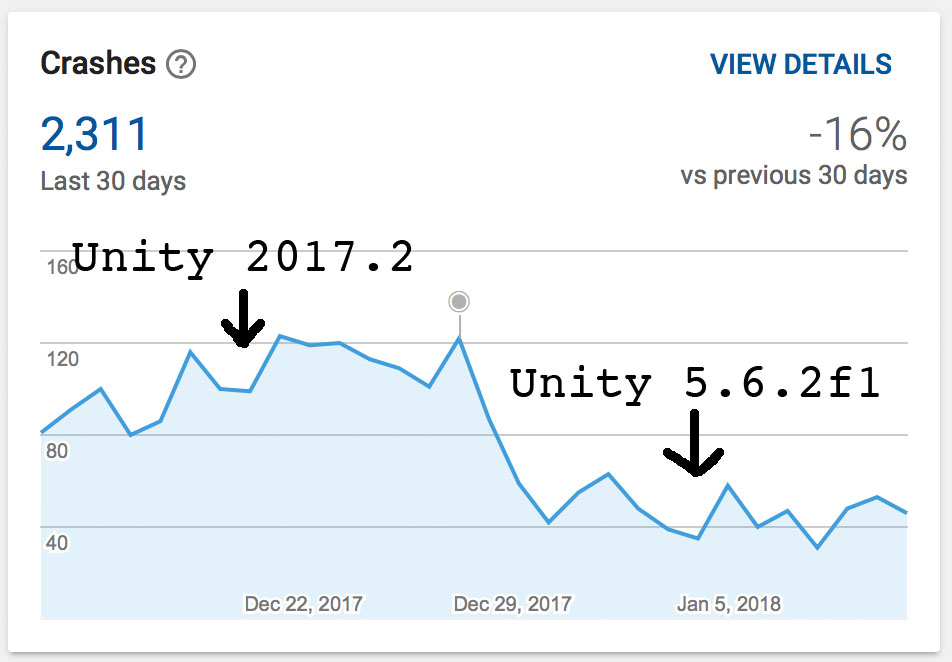
\includegraphics[width=12cm]{images/unity-forum/unity-2017-2-android-vitals.jpg}
    \caption{Unity 2017.2 Android-Vitals annotated graph (\url{https://forum.unity.com/threads/unity-2017-2-crashes-vs-5-6-2f1.511995/}}
    \label{fig:unity-2017-2-android-vitals-annotated-graph}
\end{figure}


\subsubsection{Android App Bundling}~\label{kiwix-android-app-bundling-crashes}
MUST-DO complete this section

MUST-DO Discuss the augmented crash stack trace utility, how it works, and why we did~\emph{not} use it in Google Play apps.


\subsection{Lessons learned from this case study}

As~\citep{kidwell2015_toward_fault_taxonomy_application_of_software_analytics} notes, previous research by~\citep{weider1998_software_fault_prevention_in_coding_and_RCA} nearly half the faults were introduced during coding and \emph{``...many of the faults were preventable"}. These results were borne out in the Kiwix Android case study where some of the most frequent crashes were null pointer errors in the Java code. For the Kiwix Android project one of the longer term challenges was the youth of many of the volunteer contributors including some of the development leads who were often teenagers and pre-undergraduate level software developers who wouldn't have the expertise expected of professional software developers\footnote{(They often joined via Google Code-in~\citep{google_code_in_archive} or Google Summer of Code~\citep{google_summer_of_code}).}. While there may well be training techniques and software tools, including Android Lint, that may have been able to find some of the causes of the crashes reported by Android Vitals it's unlikely that these volunteers would choose to use those tools or want to undergo training. And as interviews with developers demonstrated the perceived effort of dealing with static analysis reports and the volume of false positives mean developers don't use static analysis tools very often to find bugs~\citep{johnson2013_why_dont_devs_use_static_analysis}.

%\subsection{Summary of Kiwix Android Case Study}
\subsection{Overall evaluation of the Kiwix case study}
Within five months the project was able to reduce the crash rate of the core application from over 3\% to around a tenth of that figure. One of the main causes was the focus on addressing the most prevalently reported crash clusters in Android Vitals. This was not the only cause of the improvement, the software was also being revised and updated, this included replacing some of the existing Java code with Kotlin equivalents. 

Empirical research in Android apps that migrate from Java to Kotlin indicate the code quality often improves in tandem according to static analysis of the binary files of various releases of the studied opensource apps~\cite{GoisMateus2019_an_empirical_study_on_the_quality_of_android_apps_in_kotlin}. That work does not investigate exceptions or crashes, it does include the Kiwix Android project~\footnote{Kiwix is listed as one of the projects their research investigated:~\url{https://github.com/UPHF/kotlinandroid/blob/master/docs/fdroid_all.md}.}. However, their research predates both my case study and when the Kiwix codebase transitioned to Kotlin.

The Kiwix Android project team continued to file bug reports and address them, for instance {\small~\href{https://github.com/kiwix/kiwix-android/issues/2104}{\texttt{github.com/kiwix/kiwix-android/issues/2104}}} 
provides an example of the lead developer raising a bug report for a crash reported by Android Vitals; and \\{\small ~\href{https://github.com/kiwix/kiwix-android/issues?q=is\%3Aissue+\%22crash+report\%22+}{\texttt{github.com/kiwix/kiwix-android/issues?q=is\%3Aissue+\%22crash+report\%22+}}} provides an up-to-date view of issues labeled with ``crash report". 

In conclusion, addressing crash reports was performed actively by the developers and the crash rate of all the updated Android apps updated since the start of the case study did improve. However, following the loss of the (professional) lead developer the crash rate of the flagship app has increased, and may not decrease unless the project team take ownership of addressing the causes of the increased crash rate.

%%%%%%%%%%%%%%%%%%%%%%%%%%%%%%%%%%
\par\noindent\rule{\textwidth}{0.4pt}
%%%%%%%%%%%%%%%%%%%%%%%%%%%%%%%%%%

Confounding factors, in the discussion chapter. e.g. the observations of the crash rate increasing, the change of lead developer. Gains are not permanent, and need active engagement. c.f. more recent Kiwix data shows... ditto Catrobat.


\clearpage

\section{Catrobat Android Apps}
\label{section-catrobat-case-study}


%%%%%% Be brief if this confirms work in previous case studies.

\subsection*{Rationale}
%\marian{Need to connect this case study with the thesis: what was the goal and show the key contributions. Rationale for this case study. which gave me the chance to look at .... Rationale for the intervention.}

This case study provided an opportunity to perform a similar exercise to that in the Kiwix case study with an unusually well researched and mature mobile app. The app and its ecosystem were significantly more complex than Kiwix, which is a far simpler app in terms of codebase, development practices, and functionality. 

Like Kiwix, the core Android app had chronic and ongoing high crash rates that far exceeded the bad behaviour threshold of 1.09\%. The immediate goal was to find out whether a hackathon would enable the development team to find and address at least some of the most common run time failures in their flagship mobile app, Pocket Code. 

The key contributions to the PhD research were the hackathon and the improvements that were made in the stability of the Pocket Code Android app in the two months that followed the hackathon. The case study also contributed insight into the retiring Fabric Crashlytics mobile analytics service and the replacement, Firebase Crashlytics, and how their reports and capabilities compared with those provided by Google Play Console with Android Vitals.

The rationale for the intervention was to try and tackle a perennial challenge with the Pocket Code's quality in terms of its poor reliability/stability.

This case study built on the experiences of the Kiwix case study in several relevant ways:
\begin{itemize}
    \item To evaluate the replicability of being able to improve the stability of Android apps with another team and codebase.
    \item With the researcher playing a different role, of coach rather than being embedded in the core development team. Would the development team be able to make the improvements themselves?
    \item It included in-app crash analytics using another analytics tool which provided the opportunity to compare and contrast what the tools provide the development team and their respective utility. 
    \item The Fabric Crashlytics SDK provided the ability for developers to report handled exceptions `Errors' a feature unavailable from Google's Android platform analytics.
    \item It enabled the evaluation of a shorter hackathon approach to applying analytics to improve reliability.
\end{itemize}


\akb{Suggested general structure for the case studies: §1 Introduction (Highlight key features of case, similarities and differences w.r.t. other cases); §2 Context (Product/Project overview, Developer characteristics, tools, methods, key challenges for product/project); §3 Analytics intervention (Describe what you did with analytics in the context of the case); §4 Outcomes (Describe the outcomes resulting from the intervention); §5 Discussion (Explore what these outcomes mean for the use of analytics in mobile software more generally)}

Common attributes of Kiwix and this project include:
\begin{itemize}
    \item They are large, mature opensource projects with multiple Android apps that share some code in common. 
    \item Note: there are also separate distinct codebases for additional platforms however these were excluded from this research.
    \item They are developed by a mix of participants with a wide range of development skills.
    \item They both participate in Google's \href{https://summerofcode.withgoogle.com/}{Summer of Code} program
    \item They both have some paid development work done as a seamless part of the overall project in terms of the team structures, ways of working, and so on.
\end{itemize}

The rationale for the intervention (what I did) was to explore whether improvements could be made with as little as a day of coaching an existing development team without other material changes to their current testing, use of code quality tools, or release practices. The coaching was to help them use existing analytics data they already had available where the focus would be on establishing changes they could make to the application's source code to address various crashes and ANRs.

\subsection*{Contributions of this case study}



\setminted{fontsize=\small,baselinestretch=1}

\subsection*{Evidence}
  \begin{minted}[
    gobble=4,
    frame=single,
    fontsize=\tiny,
    breaklines=true
  ]{yaml}
    evidence available :
      vitals-scraper : ~/sandbox/vitals-scraper-logs/android-stability-analysis/data/from-android-vitals
      google-play-console-reports : ~/Dropbox/Google Play Console Reports/reports/catrobat/pocketcode/crashes
      various-materials : in Dropbox
      co-written-paper : WAMA 2019
    evidence-needed : 
      Releases and their release dates.
      Latest status of the tickets raised at the hackathon.
      Current stability metrics for the 2 apps.
      Check the evidence I have from Fabric Crashlytics and the comparisons I made between the results of both Fabric and Google Play Console.
  \end{minted}

%%%%%
% Stuff on minted
% https://tex.stackexchange.com/questions/35546/minted-setstretch-and-font-size
% https://tex.stackexchange.com/questions/484788/how-to-change-overall-font-size-of-minted
% https://tex.stackexchange.com/questions/399340/change-font-size-in-minted
% https://tex.stackexchange.com/questions/531738/minted-environment-not-working-in-overleaf
% https://tex.stackexchange.com/questions/132849/how-can-i-change-the-font-size-of-the-number-in-minted-environment
% Revisit the following if I include minted more often https://tex.stackexchange.com/questions/103141/set-global-options-for-inputminted


\subsection*{Abstract}
During a 1-day hackathon with six of the core development team for the Pocket Code Android app we applied an intervention by changing the working practices of these developers. They were asked to address the top ten crashes and top ten ANRs for the app using reports provided in Android Vitals.  The team worked on a subset of these 20 issues during the hackathon and in the following weeks. The crash rate was halved within 2 releases of the app and six weeks of the hackathon. 

\marian{Needs a sense of the change was that was introduced by my intervention. Focal points of analysis: were the developers ignoring stuff? did their behaviour change? \textbf{I need to add the researcher point of view}. Make explicit the utility of the analytics, there are early signs in~\href{catrobat-case-study-findings-and-results}{\nameref{catrobat-case-study-findings-and-results}}.}

The improvement was particularly impressive as the team's clean coding practices and their sophisticated `best practices' had not managed to effect a similar improvement in the previous months. Further scope for improvement is likely. However, the improvements petered out after the the owner for runtime stability left the team shortly after these two releases were deployed. New stability issues have emerged in more recent releases, indicating a tendency to entropy in codebases and their products unless runtime failures are actively monitored and addressed.

Changes enforced by Google led to the migration from Fabric Crashlytics to Firebase Crashlytics for reporting purposes. The team discovered personal information was being collected and reported by Google \textit{despite the Crashlytics SDK remaining unchanged and intended only to report on crashes and errors}. The project leader chose to stop actively using Crashlytics in the project as a result in order to protect the privacy of the end users.

Aspects of this case study were published and presented at WAMA 2019 in~\citep{harty_better_android_apps_using_android_vitals} and I also released a data set to make it freely available to the research community~\citep{harty_wama_dataset_examples}. 
 
% Applying advice from https://nssmic.ieee.org/2019/wp-content/uploads/sites/2/2019/02/Abstract_Style_Guide.pdf
% See also https://conferences.ieeeauthorcenter.ieee.org/write-your-paper/structure-your-paper/ 


\subsection{Introduction to the Catrobat Case Study}
% Joe's notes this is not compelling and doesn't compare with the other case studies.
% Why Catrobat, what did I gain, similarities and contrasts, why include in the PhD.
% Existing best practices, assiduously applied didn't reduce the crash rate, my approach did! :)
% Needs to be applied on a long term basis.

The Android app in this case study is an extremely and unusually well researched and properly developed app and codebase. The project started in 2010, has had over 1,300 contributors, 4 million downloads, and 350 thousand active users, and is used in 180+ nations in 60+ languages~\citep{catrobat_project}. There are at least 216 contributors for the Android Pocket Code app~\citep{github_catroid}.

Many perceived good practices were and are assiduously applied on an ongoing basis, for instance:~\href{https://github.com/Catrobat/Catroid}{Test-Driven Development, Clean Code}~\citep{catrobat_first_steps_into}, a documented consistent~\href{https://github.com/Catrobat/Catroid/wiki/Workflow}{workflow} and \href{https://github.com/Catrobat/Catroid/wiki/Creating-a-pull-request}{Pull Requests}, and \href{https://jenkins.catrob.at/job/Catroid/}{Continuous Integration}. The codebase is far more complex than the Kiwix Android apps and the app is significantly richer in terms of the features and functionality~\citep{mueller2019_pocketcode}.

This case-study includes some in-app analytics, in the form of a crash reporting tool called Crashlytics. This additional source of analytics identified additional concerns with analytics tools as the two sources of analytics (Google Play Console and Crashlytics) had significant differences in their calculations and reports. It illustrates the efficacy of investigating crashes reported by the analytics where relatively minor effort was needed to identify and fix causes of poor reliability.

The case study included two main events, 1) a hackathon in November 2019 and 2) participation in a pre-conference workshop in Poland in February 2020. 

The hackathon was mooted % in August 2019
following the success of the hackathon for the Kiwix project as a fresh intervention for the Catrobat project team to see if it would foster and encourage the development team to address at least some of the top issues that adversely affected the stability of the Pocket Code Android app. The focus was to improve code quality based on failures and issues reported in Android Vitals (cross-referenced with those reported in Fabric Crashlytics). The workshop was intended to foster collaboration between software testers and the development team while also using mobile analytics that incorporated mobile analytics into the workshop.

\subsection{Context}
% Temporal aspects, duration and nature of the engagement, 
% Consider providing a per- case-study timeline. Use dots to indicate the ongoing engagement. Use bars to indicate when I was actively involved.

\subsubsection{Product overview}

\subsubsection{Project overview}
\keywords{History, University led, combined user focus with learning, and research focus, 2 core apps, several custom apps, ...}

\newthought{Potted History of the Project}
TODO Discuss with Marian, Arosha and Yijun on whether this material is useful for providing context.
\begin{enumerate}
    \item Rationale:
    \item Involvement of under-grads and post-grads. Master's theses: (at least 8 published theses focus on the Catrobat project~\footnote{Available from \url{https://diglib.tugraz.at/search}.}).
    \item External contributors: translations, rich community contributions of PocketCode apps, ...
    \item Catrobat foundation, and funded work.
    \item Software Development, testing, maintenance,...
\end{enumerate}

\subsubsection{Developer characteristics}
\newthought{Catrobat Software Engineering Practices}
Approach to development, testing, deployment, production monitoring, ...

The project uses Jenkins to run continuous builds for PocketCode and other related projects \url{https://jenkins.catrob.at/job/Catroid/}. Most of the builds are for the Develop code branch \url{https://jenkins.catrob.at/job/Catroid/job/develop/}. The deployment practices have also been streamlined by combining Jenkins and Fastlane where various tasks people find tedious and are error-prone were automated to reduce deployment errors~\citep{luhana2018streamlining}.

The project applies various forms of test automation including unit, integration, and UI tests~\citep{luhana2018streamlining}. In addition they incorporate Behavior Driven Testing (BDD), described in detail in~\citep{ali2019using_catrobat}; and the project also uses Cucumber to automatically test the support for BiDi (\underline{Bi}-\underline{Di}rectional) text in the user interface~\citep{ayyal2016automated_bidi_testing, awwad2017_automated_bidi_testing, ali2019behavior_catrobat}. To provide some perspective, they would be one of the top few ranked projects in terms of using automated tests compared with the survey of developers of opensource Android apps~\citep{linares2017_how_do_developers_test_android_apps}, and given the project's investment in custom visual testing tiles in addition to all the other forms of automated testing could be argued to be preeminent across all the opensource Android projects. 

\newthought{The Project's Working Practices}
% Try to include examples of the human aspects and the game
Specific roles, who can do what.
Issues need to be reported in JIRA in order for any code to be considered



\subsubsection{Tools}

\newthought{Introduce the Analytics Tools}
\begin{enumerate}
    \item Types of crashes: Soft crashes (mapping terminology between Fabric Crashlytics and Android Vitals).
\end{enumerate}

\subsection{Analytics intervention}
% (Describe what you did with analytics in the contextof the case)


\subsubsection{Methods}
% It should include a statement of the main focus of the case study, as well as 'what you did'.
% Observations of the developers, looking at the code, what I did with the evidence the data collection
The main focus of this case-study was twofold: 1) to evaluate whether a hackathon driven by existing analytics would help the team materially improve the quality in use of their more complex Android app, and 2) to investigate Fabric Crashlytics as an additional source of analytics about the (un-) reliability of the app.

The approach, jointly selected by the project lead Professor Wolfgang Slany
and myself as the primary researcher,
was to co-organise a hackathon in Graz, Austria at the project's parent university, planned for 24 hours from 9am on \nth{16} November 2019. We agreed to invite and include an individual who combined extensive experience of hosting and leading hackathons with his nimble, rapid software development expertise. This individual would help to add vigour to the hackathon as the project team was not familiar with hackathons and would benefit from additional encouragement from a fellow developer who `knew the ropes' while also `demonstrating by example'.

We further agreed to two optional introductory sessions on the day before, the~\nth{15} November 2019. In the morning I would present a combination of topics related to mobile app quality, experiences of working in industry, and using analytics to improve software quality. In the afternoon a group of us would visit one of the industry leaders in system-wise monitoring, management and analytics who had a regional office nearby.

\subsubsection{Key challenges for the project/product}

\subsection{Findings}
% reporting on the data I collected
\subsection{Findings and Results of the Case Study}
\label{catrobat-case-study-findings-and-results}

Android Vitals `Bad Behavior' alerts colour coded and intended to help developers quickly notice and respond to high error rates, as illustrated in Figure~\ref{fig:android-vitals-pocketcode-alerts-23-jan-2020}. %Evidence AppHealthOverviewPlace_8841632091579025670_org.catrobat.catroid_1579796386172.png

\begin{figure}
    \centering
    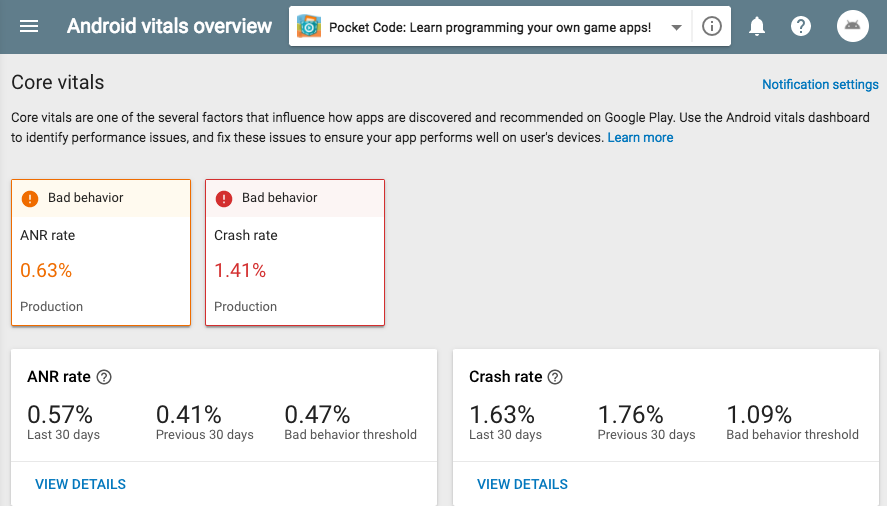
\includegraphics[width=12cm]{images/google-play-console/android-vitals-pocketcode-alerts-23-jan-2020.png}
    \caption{Android Vitals overview, bad behaviours (Pocket Code example)}
    \label{fig:android-vitals-pocketcode-alerts-23-jan-2020}
\end{figure}

No plots for either Pocket Code or Pocket Paint for the ANRs and for the crashes on \nth{10} February 2020, as illustrated in Figure~\ref{fig:android-vitals-pocketcode-broken-graph-10-feb-2020}. 
%Evidence AppHealthDetailsPlace_8841632091579025670_org.catrobat.paintroid_1581848687528.png and AppHealthDetailsPlace_8841632091579025670_org.catrobat.catroid_1581848687528.png and AppDashboardPlace_8841632091579025670_org.catrobat.paintroid_1581848687528  

\begin{figure}
    \centering
    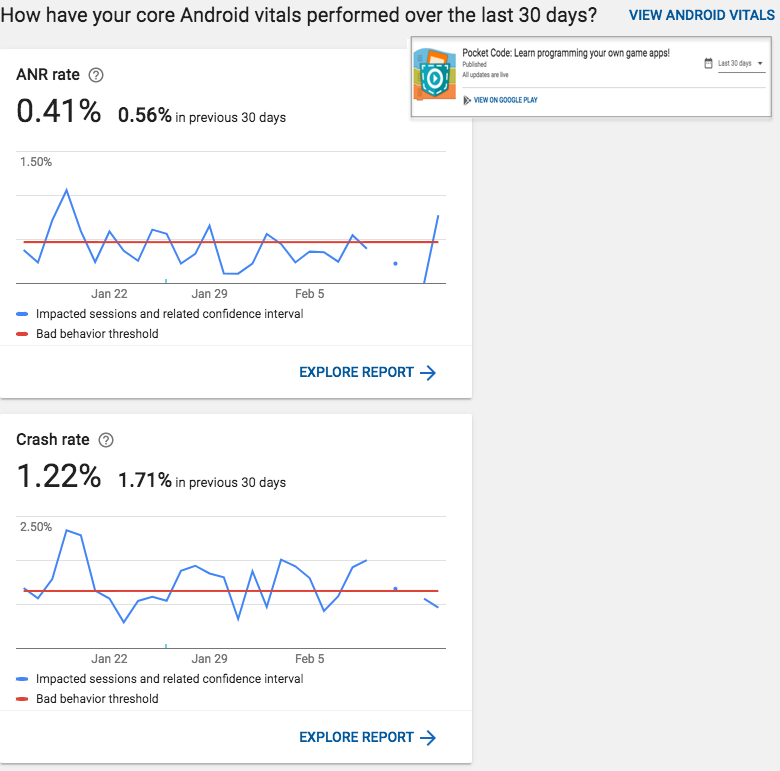
\includegraphics[width=10cm]{images/google-play-console/android-vitals-pocketcode-broken-graph-10-feb-2020.png}
    \caption{Android Vitals graph data missing for~\nth{10} Feb 2020 (Pocket Code example)}
    \label{fig:android-vitals-pocketcode-broken-graph-10-feb-2020}
\end{figure}
Illogical results for installed userbase. %Evidence various graphs.



\subsubsection{Peer Groups}
The Pocket Code Android app had a significantly higher crash-rate compared to its peer group, as Figure \ref{fig:pocketcode_peer_crash_rate_18_nov_2019} shows in section \href{android-vitals-peer-groups}{\emph{\nameref{android-vitals-peer-groups}}} shows. While this may be undesirable, the Pocket Code app had incredible richness and complexity compared to the perceived peer apps; for instance it includes support for generating native Android apps, an app store, generation of rich, graphical games, as examples of some of the rich capabilities on offer.



\subsection{Results/Outcomes}
% (Describe the outcomes resulting from the intervention e.g. Impact on the reliability of the app, changes in the behaviour of the dev. team)

\begin{figure}
    \centering
    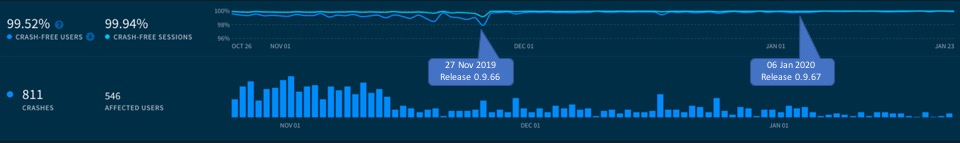
\includegraphics[width=16cm]{images/annotated_pocketcode_90_day_fabric_crashlytics_report.jpg}
    \caption{Annotated improvements with key PocketCode app releases}
    \label{fig:annotated-improvements-pocketcode-app-releases}
\end{figure}

\begin{figure}
    \centering
    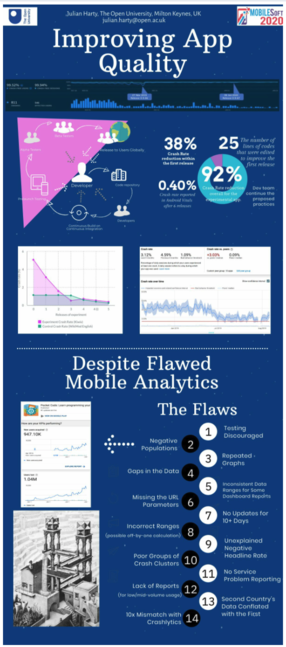
\includegraphics[width=6cm]{images/mobilesoft/resized-mobilesoft2020-poster.png}
    \caption{MobileSOFT 2020 Poster}
    \label{fig:mobilesoft2020-poster}
\end{figure}

\textbf{MUST-DO} write up and include the various images here and in the kiwix case study from the MobileSOFT2020 materials (e.g. from Figure~\ref{fig:mobilesoft2020-poster}) as appropriate.

\subsubsection{Summary of the Hackathon}
The visit (including the presentation at the Graz University of Technology on Friday morning and to Dynatrace\footnote{\url{https://www.dynatrace.com}} on Friday afternoon) helped reinforce the value of creating and using the Vitals-Scraper software to preserve history. 

There was a peak of eight participants from the Catrobat team during the hackathon. This included two people %(including Wolfgang and Matthias)
in non-coding capacities. Approximate time spent. Twenty-two (22) issues were raised during the day (tagged: hackathon-2019)\footnote{\url{https://jira.catrob.at/browse/CATROID-426?jql=labels\%20\%3D\%20hackathon-2019}}. Most of these were created in the morning, one for each of the top crashes and ANRs as recorded and ranked in Android Vitals. 

\subsubsection{Immediate outcomes post Hackathon}
We can group the issues using as follows (already fixed, addressed during the hackathon, pending, rejected).

\subsubsection{Already fixed} JIRA issue 405\footnote{\url{https://jira.catrob.at/browse/CATROID-405}} was the \#1 issue with over 2000 crashes reported in the 30 days preceding the hackathon (and over 3200 in the lifetime of the app). However, it had already been addressed in JIRA issue 379\footnote{"media download progress dialog crashers" \url{https://jira.catrob.at/browse/CATROID-379}} and incorporated in to the most recent release \footnote{Release:
0.9.65 Nov 13, 6:01 PM: Full rollout.} as part of a major effort to improve the code quality around the embedded WebView component.

Early indications are that the fixes related to the WebView have made a material improvement in the crash-rate for PocketCode 2.45\% vs. 3.9.3\% on Monday \nth{18} November 2019; details are in Table \ref{tab:androidvitals_rollout_of_0_9_65}. Therefore, in terms of assessing any improvement that results from the work of the hackathon the baseline is 2.45\%.

% TODO perhaps move these to a Glossary section?
% Number of sessions tool-tip: Approximate number of recorded sessions
% Crash-free sessions tool-tip: Percentage of daily sessions during which your users did not experience any crashes. A daily session refers to a day during which your app was used.
% Impacted sessions tool-tip: Percentage of daily sessions during which your users experienced at least one crash. A daily session refers to a day during which your app was used.
\begin{table}[htbp!]
    \centering
    \footnotesize
    \begin{tabular}{r|r|r|r}
        App version &Impacted sessions &Crash-free sessions &Number of sessions  \\
        \hline
        69 (0.9.65) &2.45\% &	97.55\% 	&~800 \\
        Production &&& \\
        \hline
        66 (0.9.64) &3.93\% &96.07\% 	&~3K
    \end{tabular}
    \caption{AndroidVitals: Improvement in crash-rate post WebView improvements}
    \label{tab:androidvitals_rollout_of_0_9_65}
\end{table}

The change was to remove a progress dialog for media downloads. The development team was not able to reproduce the crash according to the JIRA ticket or the code review in the pull request \#3362\footnote{\url{https://github.com/Catrobat/Catroid/pull/3362/files}}. And yet the fix seems to have had the desired effect in terms of the crash rate. The effect on the UX is not known.

\subsubsection{Addressed During the Hackathon}
Some of the issues were determined to be `soft errors' that were leaking to Android Vitals even though the app handled / recovered from them. These were addressed through the work recorded in  \href{https://jira.catrob.at/browse/CATROID-426}{CATROBAT-426}. Table \ref{tab:hackathon_2019_jira_addressed} provides a brief summary of all the issues addressed in the hackathon.


\href{https://jira.catrob.at/browse/CATROID-418}{CATROID-418 - Crash in PlaySoundAndWaitBrick.addActionToSequence} The author paired with one of the developers on this issue. It is believed to be a bug that can only occur at runtime when the user has deleted the sound file that is being used by the \texttt{PlaySoundAndWaitBrick} which raised an \texttt{IllegalArgumentException} as it cannot determine the path from the Java Object that represented the sound file for this PocketCode visual programming element. We were able to reproduce the error on a local device and implement a fix. The developer thought a similar behaviour might be the cause of the exception reported in issue \href{https://jira.catrob.at/browse/CATROID-419}{419}; this has yet to be investigated.

\begin{table}[htbp!]
    \footnotesize
    \centering
    \begin{tabular}{rll}
        JIRA Ticket &Category &Remarks \\
        \hline
        \href{https://jira.catrob.at/browse/CATROID-407}{CATROBAT-407} &NullPointerException &Soft error already handled by app. \\
        \href{https://jira.catrob.at/browse/CATROID-409}{CATROID-409} &NullPointerException &Crash in showLegoSensorConfigInfo
        \\
        \href{https://jira.catrob.at/browse/CATROID-418}{CATROID-418} &IllegalArgumentException &Crash in \\&&  PlaySoundAndWaitBrick.addActionToSequence \\
        %SHOULD_DO fix Temporary hack to wrap above text.

    \end{tabular}
    \caption{Hackathon bugs addressed during hackathon.}
    \label{tab:hackathon_2019_jira_addressed}
\end{table}

\subsubsection{Pending} 
Table \ref{tab:hackathon_2019_jira_issues_pool} summarises the issues that were raised and were not actioned during the hackathon.

Of these, \href{CATROID-410}{https://jira.catrob.at/browse/CATROID-410} and \href{https://jira.catrob.at/browse/CATROID-412}{CATROID-412}seem, as issue \href{CATROID-405}{https://jira.catrob.at/browse/CATROID-405} was, to have been fixed in the recent release 0.9.65 (69). Android Vitals shows these crashes last occurred in the previous release of 0.9.64 (66).

Similarly, issues \href{https://jira.catrob.at/browse/CATROID-413}{CATROID-413 - Crash in saveScreenshot} has not yet been reported for the current release: 0.9.65 (69).

\href{CATROID-411}{https://jira.catrob.at/browse/CATROID-411} is for an ANR (where the app freezes) when taking a screenshot. This occurs in both the previous and current releases and is currently being investigated by one of the development team.

\href{https://jira.catrob.at/browse/CATROID-413}{CATROID-413 - Crash in LineTool.draw} seems to be a long-running issue, found in releases (65), (66), and the current release (69).

\href{https://jira.catrob.at/browse/CATROID-415}{CATROID-415 - Crash in onBackPressed} is another long-running release however it is happening much more often - twenty-eight times by Monday \nth{18} November 2019 in the current release (69), versus once in release 63 (on \nth{23} October 2019. Of the crashes in (69) happened on the same day as the hackathon - perhaps the participants were triggering albeit they might not be aware of it? If they weren't aware, this might be another instance where the issue is a 'soft-error' which is handled by the app and therefore suitable for similar treatment to that proposed in \href{https://jira.catrob.at/browse/CATROID-426}{CATROID-426}?

\href{https://jira.catrob.at/browse/CATROID-416}{CATROID-416 - Crash in VisualPlacementActivity} from Android Vitals, this crash has only been reported in the current release 0.9.65 (69). It affected a range of devices and occurred on at least 2 Android versions.

\href{https://jira.catrob.at/browse/CATROID-417}{CATROID-417 - Crash in MainMenu onCreate} may be newly introduced in 0.9.65 (69). This has only been reported for a single user who experienced it 4 times. The exception is a \texttt{java.lang.ClassCastException} perhaps it's triggered by a particular PocketCode script or method call?

\href{https://jira.catrob.at/browse/CATROID-420}{CATROID-420 - Crash in resolveFileName} This was addressed two days after the hackathon and merged into the next release 0.9.66 (70). The crash was newly reported in 0.9.65 (69) and happened twice, once on an Huawei Y9 and once on an Honor 7X.

\href{https://jira.catrob.at/browse/CATROID-421}{CATROID-421 - ANR in MainMenuActivity} This ANR was reported in both 0.9.64 (66) and 0.9.65 (69) and has been reported on Android 7.0 and 7.1 on 3 distinct device models with all bar one on Xiaomi devices, the remaining crash is on a Lenovo VIBE K6 Note (K53a48), with Android 7.0.

\href{https://jira.catrob.at/browse/CATROID-423}{CATROID-423 - ANR in ProjectActivity} This ANR has also occurred in the most recent release: 0.9.66 (70). It's been reported 7 times on 4 device models in the last 30 days and on both Android 7.0 and 7.1

From the trace, perhaps it's related to taking a screenshot? Also, the queue delay can be over 18 seconds - far longer than anyone would like:

\texttt{\footnotesize{"Input dispatching timed out \\(org.catrobat.catroid/org.catrobat.catroid.ui.ProjectActivity, \\Waiting to send non-key event because the touched window has not finished processing certain input events that were delivered to it over 500.0ms ago. Wait queue length: 28. Wait queue head age: 18726.7ms.)"}}

\href{https://jira.catrob.at/browse/CATROID-424}{CATROID-424 - ANR in SpriteActivity} This ANR is also reported in newer 0.9.66 (70) and older releases, see \ref{tab:catroid_424}:

\begin{table}[htbp!]
    \centering
    \begin{tabular}{r|r|r}
Release	&Instances	&Percent \\
\hline
66	&12	&63.2\% \\
69	&6	&31.6\% \\
70	&1	&5.3\% \\
    \end{tabular}
    \caption{By app version for CATROID-424 issue}
    \label{tab:catroid_424}
\end{table}

The error summary is:

\texttt{\footnotesize{
Input dispatching timed out (AppWindowToken{c8e9f token=Token{b3ee03e ActivityRecord{4ed08f9 u0 org.catrobat.catroid/.ui.SpriteActivity t12205}}}, Waiting because no window has focus but there is a focused application that may eventually add a window when it finishes starting up.)}}

\href{https://jira.catrob.at/browse/CATROID-425}{CATROID-425 - tgkill crashes} There are various crash clusters for \texttt{tgkill}, 19 in 60 days to \nth{1} December 2019 across all versions of the app and Android versions. These have not been investigated yet. The ticket includes references to various guides to help investigate the causes.

\begin{table}[htbp!]
    \centering
    \footnotesize
    \begin{tabular}{r|l|l}
        JIRA Ticket &Category &Remarks \\
        \hline
        \href{https://jira.catrob.at/browse/CATROID-406}{CATROBAT-406} &NullPointerException &...BrickBaseType.getDragAndDropTargetList. \\
        \href{https://jira.catrob.at/browse/CATROID-408}{CATROID-408} &NullPointerException &Crash in Save Project. \\
        \href{https://jira.catrob.at/browse/CATROID-410}{CATROID-410} &NullPointerException &Crash in saveLegoNXTSettingsToProject \\
        \href{https://jira.catrob.at/browse/CATROID-411}{CATROID-411} &ANR &\texttt{StageListener.takeScreenshot} \\
        \href{https://jira.catrob.at/browse/CATROID-412}{CATROID-412} &NullPointerException &Crash in SetBackgroundEventId.hashCode \\
        \href{https://jira.catrob.at/browse/CATROID-413}{CATROID-413} &NullPointerException &Crash in saveScreenshot \\
        \href{https://jira.catrob.at/browse/CATROID-414}{CATROID-414} &NullPointerException  &Crash in LineTool.draw \\
        \href{https://jira.catrob.at/browse/CATROID-416}{CATROID-416} &NullPointerException &Crash in VisualPlacementActivity \\
        \href{https://jira.catrob.at/browse/CATROID-417}{CATROID-417} &ClassCastException &Crash in MainMenu onCreate \\
        \href{https://jira.catrob.at/browse/CATROID-420}{CATROID-420} &SecurityException &Crash in resolveFileName \\
        \href{https://jira.catrob.at/browse/CATROID-421}{CATROID-421} &ANR &MainMenuActivity \\
        \href{https://jira.catrob.at/browse/CATROID-423}{CATROID-423} &ANR &ProjectActivity \\
        \href{https://jira.catrob.at/browse/CATROID-424}{CATROID-424} & ANR &SpriteActivity \\
        \href{https://jira.catrob.at/browse/CATROID-425}{CATROID-425} &tgkill &Various crash clusters \\
    \end{tabular}
    \caption{Hackathon bugs in the "Issues Pool"}
    \label{tab:hackathon_2019_jira_issues_pool}
\end{table}

\subsubsection{Rejected}
\href{https://jira.catrob.at/browse/CATROID-422}{CATROID-422 - Crash at org.catrobat.catroid.ui.ProjectActivity.showLegoSensorConfigInfo } \texttt{(ProjectActivity.java:396)} %TODO work out why I needed to split the above to avoid a latex compile error.
This was rejected by one of the developers as they wanted to suppress the crash (which is considered one the app recovers from) through \href{https://jira.catrob.at/browse/CATROID-426}{CATROID-426}. Interestingly the 'fix' did not stop this crash from being reported in 0.9.66 (70).

\subsubsection{Permission Denials}
One of the Android Vitals "qualities" pertains to how often users deny permissions requested by an app. A low percentage (ideally zero) is their target recommendation. As Table \ref{tab:pocketcode_permission_denials} shows, PocketCode has a significant percentage of denials, 4.74\% as of \nth{18} November 2019. In discussion with the project lead % Commented out for review purposes:  , Prof. Wolfgang Slany, 
during the hackathon, this is a known consideration. The project team aims to improve the behaviour (\emph{i.e.} the design and implementation). The app currently asks users early on for permission to check the memory card in order to find PocketCode projects. As the permission dialog asks about access to read photos and videos, etc.\todo{Add screenshot and correct wording} it does not seem relevant to some users and they say no. As others have determined\todo{add references to design and timing of when to ask users things}  when and how an app asks a user has affects the outcomes.


% The following was copy-pasted from Android Vitals on 18th Nov 2019 for the PocketCode app.
% Metric 	Last 30 days 	Previous 30 days vs. peers’ median The difference between you and the peers’ median
% Permission denials Percentage of daily permission sessions during which users denied permissions. A daily permission session refers to a day during which your app requested at least 1 permission from its user. If a user makes multiple decisions for the same permission, only the final decision at the end of a day is recorded. Transparently explaining the reasons for permission requests can help reduce permission denials. 	4.74% 	4.39% 	-

% https://play.google.com/apps/publish/?account=8841632091579025670#AppHealthDetailsPlace:p=org.catrobat.catroid&appid=4975762901432177859&aho=APP_HEALTH_OVERVIEW&ahdt=PERMISSION_DENIAL&ts=THIRTY_DAYS&ahbt=_APPLICATION


  \bxtable[htbp!]{{AndroidVitals: PocketCode: "Permission Denials"}}
  {
  \begin{minipage}{16cm}
  %\begin{center}
    \begin{tabular}{lrrr}
        Metric 	&Last 30 days\footnote{As of \nth{18} Nov 2019} 	&Previous 30 days &vs. peers’ median  \\
        Permission denials\footnote{Percentage of daily permission sessions during which users denied permissions.\\ A \emph{daily permission session} refers to a day during which your app requested at least 1 permission from its user. If a user makes multiple decisions for the same permission, only the final decision at the end of a day is recorded. Transparently explaining the reasons for permission requests can help reduce permission denials~\citep{androiddevelopers2020_permission_denials}} & 4.74\% 	&4.39\% 	&- \\
   
   \label{tab:pocketcode_permission_denials}
    \end{tabular}
     % \end{center}
  \end{minipage}
  \centering
}

% Thanks to https://tex.stackexchange.com/questions/10181/using-footnote-in-a-figures-caption for the local footnotes.
% This also helped me find a viable approach: https://tex.stackexchange.com/questions/109467/footnote-in-tabular-environment
% This also looks good as an alternative: https://texblog.org/2012/02/03/using-footnote-in-a-table/
% Ditto the following threeparttable example https://blog.modelworks.ch/tables-with-footnotes-in-latex/

% And yet more reading in an attempt to quiesce nag messages (I've yet to succeed)
% https://latex.org/forum/viewtopic.php?t=31733
% https://tex.stackexchange.com/questions/237549/center-environment-nag-warning-for-floats-in-beamer

% Tables ain't trivial in latex. Finally the following article clearly explains how to use captionof minipage and tabular
% https://tex.stackexchange.com/questions/15282/tabular-title-above-and-caption-below
% and https://tex.stackexchange.com/questions/2275/keeping-tables-figures-close-to-where-they-are-mentioned

\subsubsection{1 Week on}
Release 0.9.65 is now the dominant release, with ~4000 sessions between \nth{17} and \nth{23} November, compared to ~600 sessions for the previous release of the app (0.9.64). The overall reported crash rate reduced to 2.10\% for \nth{18} to \nth{23} November, compared to the previous 7 days crash rate of 3.62\%. \textbf{Note these are for releases that predate the hackathon.}

During a call with Professor Slany on \nth{25} November, he mentioned they had planned to release a new version of the app on Friday to address the loss of Fabric Crashlytics data and several improvement related to the hackathon; however their Jenkins build was coincidentally broken that day \url{https://jenkins.catrob.at/job/Catroid/job/develop/1098/} where the build failed to complete for over 54 hours. The cause was being investigated. According to logs on Jenkins it may be related to Docker not being available \texttt{Cannot connect to the Docker daemon at unix:///var/run/docker.sock. Is the docker daemon running?} \footnote{\url{https://jenkins.catrob.at/view/Catroid/job/Catroid/job/develop/1102/execution/node/27/log/}}

\subsubsection{2 weeks on}
\nth{1} December 2019.

A new release of the app was launched on November \nth{26} after several days of problems with the Jenkins CI pipelines which delayed this release by about 4 to 5 days.

The new release 0.9.66 (70) seems to have made a slight improvement to the overall crash rate which is currently 1.95\% after 3 days of data in Android Vitals, the previous release has a crash rate of 2.56\% for the last 7 days (to \nth{29} November. It is premature to determine the overall effect of the crash rate for this app as it's still being rolled-out (which typically takes over a week to reach the majority of the user-base e.g. on \nth{2} December (4 days after the release started rolling out) Android Vitals reports 20K install events).

The ANR rate is also showing encouraging signs, for the last 7 days (actually it seems to be only for 6 days, from \nth{24} to \nth{29} November 2019 as reported on \nth{1} December 2019) in Table~\ref{tab:ANR_rate_24_to_29_Nov_2019}.

\begin{table}[htbp!]
    \centering
    \footnotesize
    \begin{tabular}{r|r|r|r}
      App version  &Impacted sessions &ANR-free sessions &No. sessions \\
      \hline
      70 (0.9.66) Production &0.30\% &99.70\%	&~700 \\
      69 (0.9.65)            &0.46\% &99.54\%	&~3K  \\
    \end{tabular}
    \caption{PocketCode: ANR rate for Last 7 days}
    \label{tab:ANR_rate_24_to_29_Nov_2019}
\end{table}

\subsubsection{Progress in cumulative releases}

% MUST_DO add screenshots and summaries of the progress made with subsequent releases of Pocket Code for Android.

\begin{table}[htbp!]
    \centering
    \footnotesize
    \tabcolsep=0.06cm
    \begin{tabular}{r|r|r|r|r}
    \small
        App version &Impacted sessions &Crash-free sessions &Number of sessions &Period \\
        \hline
        72 (0.9.68) &1.26\% &   98.74\%     &~9K  &11-Jan-2020 to 08-Feb-2020 \\
        71 (0.9.67) &1.25\% &   98.17\%     &~14K &11-Jan-2020 to 08-Feb-2020 \\
        70 (0.9.66) &1.65\% &   98.35\%     &~5K  &04-Jan-2020 to 01-Feb-2020 \\
        69 (0.9.65) &2.05\% &	97.95\% 	&~2K  &22-Oct-2019 to 19-Nov-2019 \\
        \hline
        66 (0.9.64) &3.61\% &   96.39\% 	&~16K &22-Oct-2019 to 19-Nov-2019 \\
    \end{tabular}
    \caption{AndroidVitals: Improvement in crash-rate post Hackathon}
    \label{tab:androidvitals_crashrate_post_hackathon}
\end{table}

Some notes on Table~\ref{tab:androidvitals_crashrate_post_hackathon}:
\begin{enumerate}
    \item The data was reported for thirty-day periods, one of three durations available in the user interface. All figures were calculated and provided by Google's Android Vitals analytics.
    \item The reports exclude small aggregate counts that fail to meet Google's reporting thresholds.
    \item The percentages fluctuate depending on where releases are in their maturity (their production lifecycle). Therefore these values are spot figures calculated that day and indicative rather than necessarily being suitable for calculating ratios for different periods. % c.f. https://gradcoach.com/nominal-ordinal-interval-ratio/ This point is probably worth expanding on - that it's unwise to simply compare absolute values to determine 'better' and 'worse' in terms of the quality of the actual app. Instead we're getting the equivalent of spot prices of how that release, etc. fared that period. Proivde examples from Kiwix (WebView) and the large industrial case study. Note this material should probably be in an overall chapter rather than this case study. Here we can forward reference that material.
    \item These reports appear to be regenerated once a day, roughly 24 hours apart.
    \item It is unclear whether the underlying data is filtered to limit it to apps only installed by end users of production releases from Google Play.
\end{enumerate}




\subsection{Discussion}
% (Explore what these outcomes mean for the use of analytics in mobile software more generally)
% Also address the RQ's here for this case study.
Effects of being measured is a well-known in work, business, etc. One of the effects here was that `soft-crashes' were reaching Android Vitals and therefore significantly and adversely affecting the crash rate (see \cite{CATDROID-426-JIRA}).

\subsubsection{Validity considerations}
\begin{itemize}
    \item Inconsistencies in the practices
    \item Inconsistencies in the tools
\end{itemize}

Furthermore, the project team chose to invest their energies into supporting a testing workshop in Poland and to introducing application-level in-app analytics to both their Android and iOS PocketCode apps (later reversed as explained in the discussion). Their actions indicate the project team recognise the benefits of applying and incorporating analytics into their software development and quality improvement practices.


One possible hypothesis is the team were overly focusing their efforts in pre-release activities. \citep{kitchenham1996_software_quality_elusive_target}, observed that the approach of taking a product view of quality~\emph{``is frequently adopted by software-metrics advocates, who assume that measuring and controlling internal product properties (internal quality indicators) will result in improved external product behavior (quality in use)."}~\footnote{US English spelling was used in the original article so used here in the quotation.} Would working backwards from the failures help the team address the quality in use more effectively?








\subsubsection{Slower growth of user-base}
PocketCode is an app developed to serve several challenges simultaneously, including research aspects such as the effects of various software development engineering practices, while also being intended to be open, in terms of informing the end-user of the purposes of the app, yet also being easy, fun and educational for children to use in terms of exploring how to write and publish software. These various concurrent challenges led to the users being presented with a long page of legal text (reformatted slightly from the original \href{https://github.com/Catrobat/Catroid/blob/develop/catroid/src/main/res/values/strings.xml}{\textbf{\texttt{Privacy policy on GitHub}}} and reproduced below in Listing~\ref{pocketcode-privacypolicy}). New users are expected to read and agree to before they are allowed to use the app further. Imagine having to scroll through all the text on a small screen \emph{before seeing what the app can do!} The thesis continues after the listing...

% COULD_DO there's lots of scope to tidy up this listing at some point.

\definecolor{dkgreen}{rgb}{0,0.6,0}
\definecolor{gray}{rgb}{0.5,0.5,0.5}
\definecolor{mauve}{rgb}{0.58,0,0.82}

\lstset{frame=tb,
  language=Cobol,
  aboveskip=3mm,
  belowskip=3mm,
  showstringspaces=false,
  columns=flexible,
  basicstyle={\tiny\ttfamily},
  numbers=left,
  numberstyle=\tiny\color{gray},
  %keywordstyle=\color{blue},
  commentstyle=\color{dkgreen},
  %stringstyle=\color{mauve},
  breaklines=true,
  breakatwhitespace=true,
  breakautoindent=true, 
  breakindent=1pt,
  tabsize=2,
  xleftmargin=0pt
}
\begin{multicols}{3}
% \lstinputlisting[{language=[LaTeX]TeX},breaklines=true]{\jobname.tex}

\begin{lstlisting}[caption={Privacy Policy for Pocket Code},captionpos=b,label={pocketcode-privacypolicy}]
Welcome!
Before you can start coding, please read and accept our Privacy Policy to use the app:
To offer you all the benefits of our services and the associated account, it is necessary to collect certain data from you.
* To maintain and improve our services (apps and websites) and to do scientific research on ICT and STEM/STEAM education, we use Google Analytics, Crashlytics, and Firebase, all by Google LLC (USA), as well as Dynatrace by Dynatrace LLC (USA) to get metadata about the usage of our services, e.g., crash information, timestamps, visited pages/screens, usage of our apps and services, used operating system, and information about the network provider. This analysis and the collected data is not linked to your profile and does not contain any personal information (last bits of the IP address get anonymized). However, the collected data will get transferred to the service-provider (Google LLC, USA and Dynatrace LLC, USA). 
Data processing is based on agreements with Google LLC and Dynatrace LLC. 
This relationship to the service provider conforms to the European Union\'s General Data Protection Regulation (EU GDPR) and EU-USA \"Privacy Shield\" agreement.
* To create and use an account in our systems, and to inform you about necessary changes about your account per e-mail, e.g., updates or violations of our Terms of Use and Service, our community rules, or our policies, we will store your username and, if provided by you, your e-mail address. If you have connected your account via your Google or Facebook account, we additionally store an identification key connected to your account on these services. We will not use this data for any other (e.g., marketing) purposes, unless you explicitly allowed us to do so.
* On a voluntary basis, you can give us your country of residence through your account page on the sharing site. This will get displayed on your public profile and only be used for statistical and research purposes by us. It can be removed at any time in your profile settings.
* You can withdraw the usage of the personal data belonging to your account at any time by deleting your account through your profile page on https://share.catrob.at. After deleting your account you will still be able to use the provided services, but not to collaborate, e.g., through uploading programs, commenting, or liking. Also, all provided content linked to your account, e.g., uploaded programs, comments, etc., will be deleted.
* To avoid misuse of our services, e.g., through user contributed uploads or comments for illegal purposes, all user generated public data (uploads, comments) will be stored internally in a database, together with a timestamp and the used internet address. This data will not be used by or forwarded to any institutions, unless sufficiently illegal actions are reasonably suspected and officially entitled legal institutions request it based on applicable law. Each case will be thoroughly checked on an individual basis by us first.
* You can voluntarily subscribe to the Catrobat Newsletter, on https://catrob.at/newsletter provided by us through the MailChimp service (The Rocket Science Group LLC d/b/a MailChimp, USA). You will then receive updates on the Catrobat project and its services to your provided e-mail address. You can withdraw the newsletter at any time by using the \"unsubscribe\" link in the footer of every newsletter. This newsletter is provided by MailChimp with whom we do have a data-processing agreement and who committed to the EU General Data Protection Regulation and EU-USA \"Privacy Shield\". For further details on MailChimp please also look up MailChimp\'s Privacy Policy and Terms of Use.
* All Services are provided by the free open source Catrobat project under the umbrella of the International Catrobat Association - Verein zur Foerderung freier Software, a non-profit NGO incorporated in Graz, Austria (European Union). Our policies pay respect to EU and Austrian data protection law (GDPR). To get in touch with us, please send an e-mail to contact@catrobat.org or mail us to Catrobat,
    c/o
    Institute of Software Technology,
    Graz University of Technology,
    Inffeldgasse 16b,
    A-8010 Graz, Austria
    (European Union).
In case you are below the age of 14, this policy must be accepted by a legal guardian (usually a parent).

Catrobat\'s official English language privacy policy is available on the web under https://catrob.at/privacypolicy.

Version 2.2, 17 October 2019

Find the previous, outdated, version of our privacy policy (2.0) here: http://developer.catrobat.org/privacy_policy_2-0
\end{lstlisting}
\end{multicols}
% Inspired by https://tex.stackexchange.com/questions/34098/two-column-code-listings-in-appendix-in-a-one-column-report

Welcome back. 

I hope the experience of scrolling past the privacy policy here provided you with an idea of how adding a mandatory, relatively comprehensive privacy policy interrupts the flow. One of the topics in the future work chapter, \href{enhancing-quality-vs-enhancing-ux}{\textit{\nameref{enhancing-quality-vs-enhancing-ux}}}, considers whether developers may obtain greater return on their investment by improving user experience rather than improving technical qualities of an app. As \href{enhancing-quality-vs-enhancing-ux}{Figure \ref{fig:Firebase-pocketcode-android-7-day-new-user-retention-29-may-2020}} shows, the Pocket Code app only retains 4\% of new users by day 2. Perhaps, the low retention rate may restrict the growth of the user-base even though the quality has improved markedly.

\subsubsection{Catrobat iOS Pocket Code App}
A more recent codebase, aimed at providing similar functionality to the Android Pocket Code app. This codebase is written specifically for iOS using the mainstream iOS development tools and development environment. 

In February 2020 the development lead for the iOS app, in conjunction with me and the overall project lead, decided to add Firebase Analytics to the iOS codebase and implement crash reporting and in-app analytics. This was quickly integrated and made available in an interim build of the app which also included some diagnostic features, including the ability to trigger a crash using an unusual pattern of interactions with the GUI of the app (to avoid end users accidentally triggering crashes).

%SHOULD-DO find screenshots of the crash. Update this section with links to the documentation from the test:fest hackathon.

\begin{itemize}
    \item The design document
    \item The implementation process and effort needed
    \item Early discoveries (discussed at the workshop in Poland on \nth{28} February 2020.
\end{itemize}
TBC

\section{Evaluation of the Catrobat case study}
The developers were able to significantly improve the reliability of their major Android app: Pocket Code, through applying a variation of the process identified in my research. The minor app, called Pocket Paint, is a separately packaged version of the drawing (paint) functionality in Pocket Code.

The project team were able to use two sources of analytics on crashes: Google Play Console incorporating Android Vitals, and Fabric Crashlytics. There were differences in the outputs and results of these tools, these are discussed later in this chapter, nonetheless they contained a common set of crashes and fixing the crash was reflected in both tools.

The project has a particularly and unusually mature process and focus on software quality as part of being an essential year-long module for various undergraduate courses and also used for post graduate research at Masters and PhD level. Nonetheless the crash rate was stubbornly high and exceeded Google's limit before we started the case study.

TBC

Still to do:
\begin{itemize}
    \item Intermittent focus on addressing crashes
    \item Loss of Crashlytics data for a period through a mistake configuring a release.
    \item The inclusion of Firebase Analytics in the Android app.
    \item The inclusion of Crash and Firebase Analytics in the iOS app, including ongoing work: See Firebase in iOS app https://jira.catrob.at/browse/CATTY-371?jql=text%20~%20%22firebase%22%20ORDER%20BY%20created%20DESC 
    \item Proposal to move to privacy-friendly analytics tools. 
\end{itemize}



\subsection{Codicil for this case study}
The case study started with a single core event - the hackathon in Graz and the ramifications of that hackathon. However one of the ramifications was an agreement to collaborate and participate in a subsequent workshop in Wroclaw, Poland at a conference primarily organised by and for software testers. That workshop did not go to plan for a couple of key reasons. Covid-19 had started to permeate Poland immediately before the conference which necessitated the conference organisers having to make wide-ranging major adaptions to the design of the conference and to the programme as some speakers had symptoms of covid-19. Second, the conference organisers were the bulk of the participants for the workshop and couldn't spend the time they'd intended in the workshop since they had to attend to everything else, and third some of the intended participants were asked to stay home to reduce the risk of the event becoming `a superspreader'~\citep{cave2020covid}.

\subsection{Summary of the Catrobat Case Study}
TBC

\dotfill
\subsection{Old materials follow and are available to pillage before being removed.}

\subsubsection{Opening gambit}
At the start of the case study the crash rate of the Pocket Code app remained stubbornly high despite the extensive use of code quality tools and practices, automated testing, continuous builds and so on. They also had access to two sources of crash analytics. What were they missing?
\clearpage

\section{Greentech Apps}~\label{study-greentech-apps}

\subsection{Introduction to the Greentech Apps case study}
The aims and objectives of this case study include:

\begin{itemize}
    \item \textbf{A linear increase (+1)} : validation the methods described in my research are repeatable and scale to additional apps beyond the previous case studies.
    \item \textbf{Additional examples of characteristics of Google Play Console (+1)} :
    \item \textbf{A closed source case study (?)} : The previous case studies were all with opensource codebases so the code was available for bug investigation purposes. For this case study the source code and build processes are treated as a black box (it may potentially become a grey box case study if the development team share details of their engineering practices, etc.)
\end{itemize}

\subsection{Background to the Greentech Apps case study}
A set of Android apps developed and provided by Greentech Apps Foundation. They are described as modern Islamic Applications, according to their website \url{https://gtaf.org/}. The project encourages voluntary contributions, for instance to provide translations~\url{https://greentech.oneskyapp.com/collaboration/}. Their apps are popular, and well regarded. % MUST_DO add data on usage and ratings.


The project started in 2016 with the aim of enabling people to learn the Quran in the local language - Bangla - in Bangladesh. The project was started by a self-taught Android developer and his cousin Yemin, at the time an undergraduate student in computer science, who is now employed by the project in a hybrid role of software developer and project manager. The development team was predominantly volunteers until around 2018 when the first engineer was employed. In April 2020 the development team added two part-time paid developers and there are plans to grow the employed team including someone with UI and UX expertise. The team are funded through voluntary donations. From a research perspective my contacts at the project are Yemin and a fellow PhD student Riasat who also volunteers for the project.

At the start of the case study (June 2020) the team had ten Android apps published in Google Play~\url{https://play.google.com/store/apps/dev?id=7665838187257770408}. Of these apps, three are their core apps, and a couple are overdue an engineering revamp.  Two analytics tools are used for their core apps: Firebase Crashlytics and the default combination of Google Play Console with Android Vitals.

Their development team maintain their issues lists in public (\url{https://gitlab.com/greentech/}), the source code is private. They use a variety of languages and frameworks to develop their apps include React Native for at least one app (\href{https://play.google.com/store/apps/details?id=com.taskinator}{Taskinator}) and Java for the majority, they aim to use Flutter~\cite{flutter_dev_site} in future.

Exodus Privacy~\cite{exodus_privacy_project}, a non profit organization, was used to determine which analytics libraries are embedded in which of their apps as the source code was not available for these apps.

\textbf{SHOULD-DO} reformat the following as a table, or similar. Add the rest of their apps for completeness.

\href{https://play.google.com/store/apps/details?id=com.greentech.quran}{Al Quran (Tafsir \& by Word)} includes \href{https://reports.exodus-privacy.eu.org/en/reports/com.greentech.quran/latest/}{Google Crashlytics, Google Firebase Analytics}.

\href{https://play.google.com/store/apps/details?id=com.greentech.hadith}{	
Hadith Collection (All in one)} includes~\href{https://reports.exodus-privacy.eu.org/en/reports/77502/}{Google Firebase Analytics}.

\href{https://play.google.com/store/apps/details?id=com.greentech.hisnulmuslim}{	
Dua \& Zikr (Hisnul Muslim)} includes~\href{https://reports.exodus-privacy.eu.org/en/reports/54714/}{Google Firebase Analytics}. This app is available in two primary languages, English and Bangla (the mother tongue of where the core development team live, in Bangladesh). The \href{https://play.google.com/store/apps/details?id=com.greentech.hisnulmuslimbn}{Bangla} version of the app is several times more popular than the English release. Unlike the English version, the Bangla version of the app includes~\href{https://reports.exodus-privacy.eu.org/en/reports/146430/}{Google Crashlytics, Google Firebase Analytics}.

\href{https://play.google.com/store/apps/details?id=com.taskinator}{Taskinator} uses~\href{https://reports.exodus-privacy.eu.org/en/reports/146496/}{Firebase Analytics, OneSignal}.

Additional analysis by the researcher in July 2020 is available online in a Google Document that has been shared with two core members of the project team amongst others~\url{https://docs.google.com/document/d/1Ghu0UBXNrwOB3HYbgsPQ-OJV-fPmsP68lSLVRfcc4aA/edit?usp=sharing}.

\subsection{Development microcosm}
Who, how, where source and bug tracking take place. 

When do teams decide to fix which bugs, and what influences their decision making process?

NPE's and IndexOOBExceptions vs. IllegalStateException and native crashes.

The team have used Firebase TestLab to test some of the apps occasionally and the Robo testing performed automatically by the test lab has triggered various crashes in the apps being tested. One such example was where an app was missing a `resource'. The team fixed the build by adding the missing resource but did not explicitly retest the app afterwards in Firebase. 

\subsection{Applying analytics to the development practices}

The development team check Android Vitals approximately once a week, and Firebase more frequently as the team decided the crash reports in Firebase are more actionable. Perhaps unsurprisingly they check more often after new releases of their apps looking for any new bugs arising in the new release as it rolls out across the user population.



Differences noticed in their reports, however the focus is on the crashes reported in Firebase as they contain more contextual detail. ANRs seldom checked, considered to be less impactful on users and lower frequencies.

\subsubsection{Worked examples}
\textbf{This section needs redoing as the discussion with Yemin indicates they use Firebase predominantly}.
These worked examples are taken from Android apps developed and maintained by the Greentech team. They are taken on the \nth{7} and \nth{8} September 2020. They exemplify various aspects of the~\href{section-select-aggregate-scope-analyse-triage-and-prioritise}{\MakeLowercase{\emph{\nameref{section-select-aggregate-scope-analyse-triage-and-prioritise}}}} section. % SHOULD-DO find out why the section name still has an initial capital letter.



\subsubsection{Preserving the failure clusters}
Details of the crashes are recorded in individual issues on the respective project's GitLab site. The issue is cross-referenced in a note in the crash cluster reported in Firebase.

\subsection{Priorities of the project team}
Throughout 2020 and until April 2021 the team are focusing on bug-fixes which include fixing the causes of crashes in the apps. Three of the apps (four as one app is released as two distinct binaries) are in ongoing active development (\href{https://play.google.com/store/apps/details?id=com.greentech.quran}{Al Quran},~\href{https://play.google.com/store/apps/details?id=com.greentech.hadith}{Hadith Collection}, and~\href{https://play.google.com/store/apps/details?id=com.greentech.hisnulmuslim}{Dua \& Zikr}, which is also released separately in Bangla~\href{https://play.google.com/store/apps/details?id=com.greentech.hisnulmuslimbn}{{Dua and Zikr (Hisnul Muslim)}}~\emph{in Bengali}); and they plan to revamp two more of the apps (\href{https://play.google.com/store/apps/details?id=com.greentech.islamicquiz}{(Islamic Quiz)} and~\href{https://play.google.com/store/apps/details?id=com.greentech.salatbn}{Meaningful prayers (salat)}~\textit{in Bengali}, which was called salat in our interview).

% SHOULD-DO add support somehow for Bengali Unicode so I can replace the Anglicised app names with the correct ones. The issues are a mismatch between the compiler I'm using (pdfLatex) vs. the recommended packages to use
% e.g. 
% https://tex.stackexchange.com/questions/285507/how-can-i-use-bengali-script-in-an-english-document
% https://tex.stackexchange.com/questions/99606/how-to-write-bengali-in-latex
% https://www.overleaf.com/learn/latex/Multilingual_typesetting_on_Overleaf_using_babel_and_fontspec
% https://www.overleaf.com/learn/latex/international_language_support#Babel
% %%%
% https://www.researchgate.net/post/How_to_write_Bengali_unicode_text_in_English_document_in_Latex
% https://www.overleaf.com/learn/latex/arabic


\subsection{Summary of the Greentech Apps case study}
TODO complete this section, reflecting the topics raised in the introduction to the case study.
Integrate their comments on reducing the crashes and using analytics \url{https://gtaf.org/blog/gtaf-accomplishment-2020}.
\clearpage

\section{Field Reports from Commercial App Developers}~\label{section-field-reports-case-studies}
The research includes field reports from developers of three distinct commercial Android apps. Each uses mobile analytics in their regular software development practices.

\subsection{Characteristics of the commercial apps}

\begin{itemize}
    \item Technologies
    \item Analytics available to the team
    \item Development priorities for their use of analytics
\end{itemize}

\subsection{Moonpig}

\begin{figure}
    \centering
    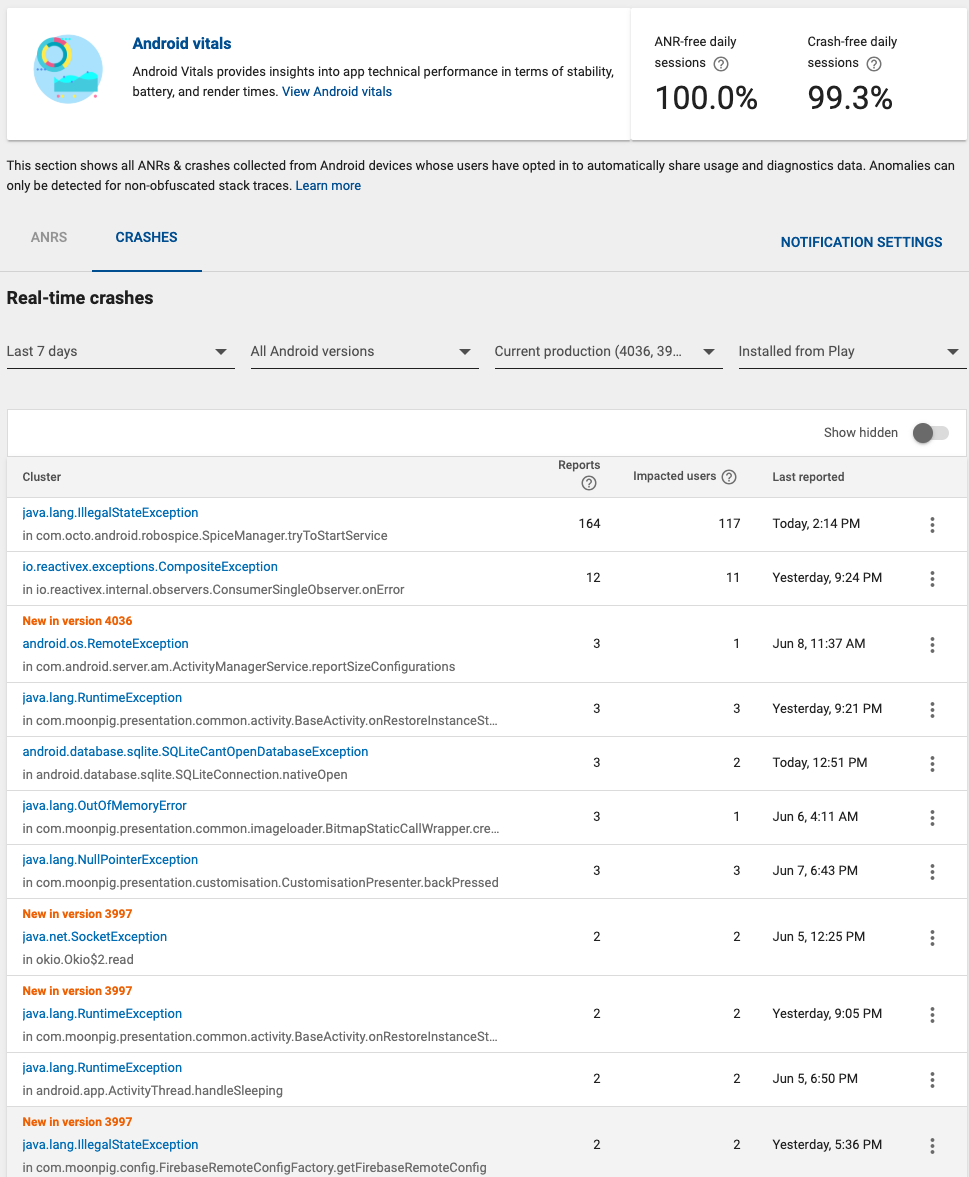
\includegraphics[width=13cm]{images/android-vitals-screenshots/moonpig/real-time-crashes-Screenshot-2019-06-10-at-15.42.34.png}
    \caption{Android Vitals: Moonpig snapshot of top crashes \nth{10} June 2019}
    \label{fig:av-moonpig-top-real-time-crashes-10-jun-2019}
\end{figure}

In Figure~\ref{fig:av-moonpig-top-real-time-crashes-10-jun-2019} Android Vitals shows the most frequent crash clusters for the production releases of the Moonpig Android app. The majority of crashes were an \texttt{IllegalStateException} in a third-party library SpiceManager, part of the RoboSpice opensource project https://github.com/stephanenicolas/robospice . 

This crash is an excellent example of how changes and new developments in the ecosystem can render what was reliable working software into software that is no longer fit for purpose, \emph{i.e.} RoboSpice was developed in 2012 to help developers simplify coding of asynchronous networking requests https://github.com/stephanenicolas/robospice and the library worked really well at the time and for several years afterwards. It became popular as a result and was used widely by many teams, including at Moonpig. However, as the Google Android platform morphed some of the changes to Android were incompatible with RoboSpice. And with Android Oreo (Release 8.0) changes to the way background services worked broke the functionality of the library sufficiently that the project was archived by the creator and project owner https://github.com/stephanenicolas/robospice/issues/467 

For apps that used RoboSpice the crash rate increased on the newer releases of Android, for example Figure~\ref{fig:av-moonpig-crash-rate-groupings} shows the crash rates by Android version were lowest on Android 7, higher for Android 8 and 8.1, and significantly higher again for Android 9. The teams needed to allocate time and energy to finding a suitable alternative to RoboSpice and then implement and test the new approach. Android Vitals helped provide an indication of the effects of the crashed and therefore provided evidence the development team could use to assess and prioritise the work.

\begin{figure}
    \centering
    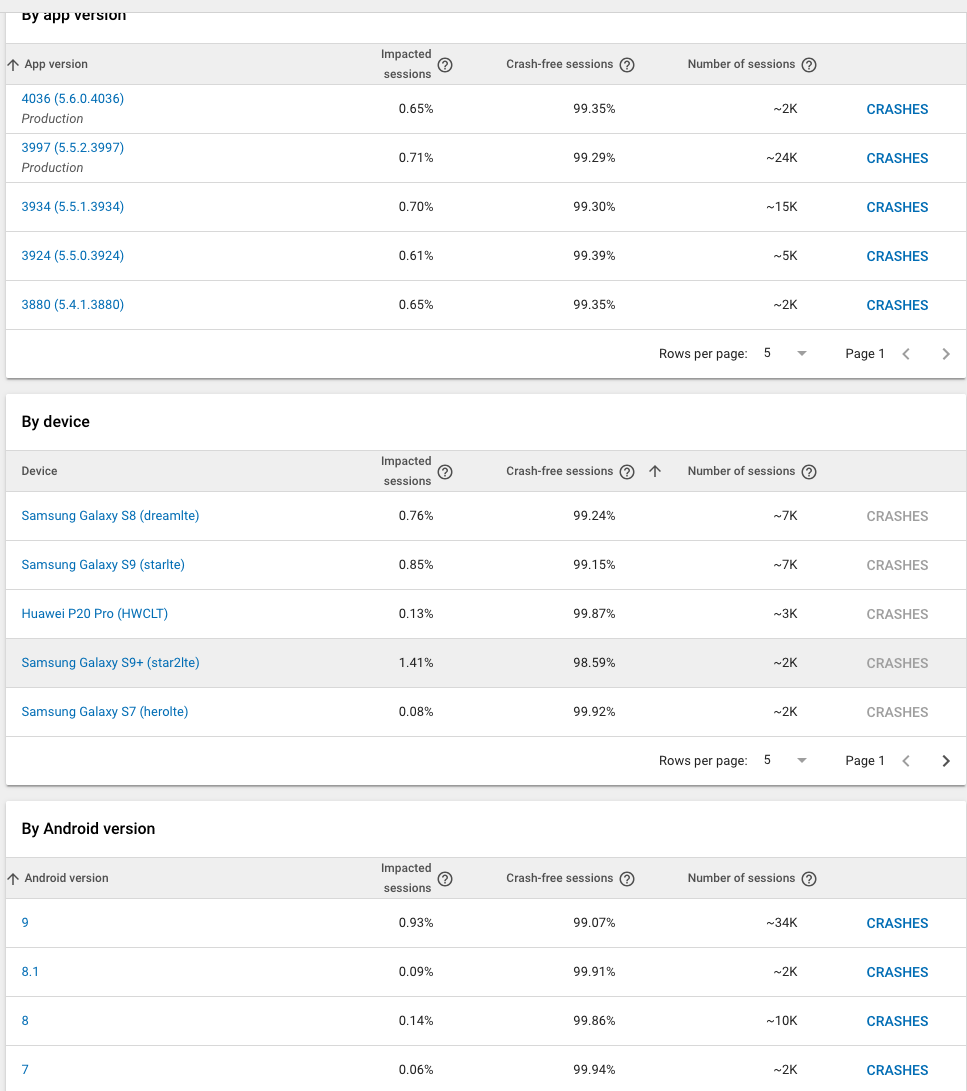
\includegraphics[width=13cm]{images/android-vitals-screenshots/moonpig/Screenshot 2019-06-10 at 15.41.23.png}
    \caption{Android Vitals: Moonpig various groupings of the crash rate \nth{10} June 2019}
    \label{fig:av-moonpig-crash-rate-groupings}
\end{figure}

\subsection{Moodspace}
Moodspace is an Android app aimed at improving mental health through various exercises incorporated into the app. It was released in 2019, with over 150K downloads by early 2020~\citep{objectbox2020_moodspace_interview}. Ian Alexander, the interviewee, was the software developer, co-founder, and runner of the company~\citep{objectbox2020_moodspace_interview} so he combines technical and operational responsibilities. He is an experienced app developer and also trained as a chemical engineer.  % https://www.linkedin.com/in/ian-alexander-01353340/

(\nth{13} June 2019)
% Source https://mail.google.com/mail/u/0/?q=kiwix+crash+rate+#search/kiwix+crash+rate/KtbxLzGHgCVznXxsGDjVgJGLFwmmGXxvxq
I love Android vitals - especially \textbf{core vitals}. Seeing your app in comparison to apps of peers provides some great motivation to step up your game. The only issue I have with core vitals is that I can't see them all! We are by no means a big app, so don't have enough data to meet googles standard for anonymised results, so results for most of the core vitals are hidden. I don't quite understand why this should be the case as the headline figure of your apps performance surely doesn't have to rely on anonymous data? Whereas the drilled down details of a core vital should be anonymous, so maybe the details view could just be blocked instead of hiding the entire core vital? To give context, MoodSpace has at least 4k monthly users, so there must be plenty of apps which get little or no use form core vitals, simply from them being hidden.

As for the other tools Google provides:
\begin{itemize}
    \item \textbf{ANR \& crashes} - I usually use crashlytics, so never really use this tab. the reason being, that the play console used to be very unreliable for crashes. But by the looks of it, it seems to have improved a lot, and pretty much matches the crashes I see in crashlytics now. Looking at it now, I actually noticed an ANR which could probably be fixed!
    \item \textbf{Pre launch reports} - I don't usually use this. Although this tool provides a nice safety net, it's quite basic, so any bugs that would cause the pre launch tests to fail have been found pre uploading through some quick manual testing. I actually ended up ignoring most pre launch reports when accessibility problems used to trigger failures, as we don't really have the resources to handle accessibility for now. But this seems to have changed in the last few months and accessibility problems don't cause a host of errors - maybe a way to ignore issues would be useful? In fact, pre-launch reports currently don't run on my app and fail with an incompatible apk error, not too sure why thats the case...
    \item \textbf{App signing} - very useful! and always use this since it was added.
    \item \textbf{Seperate release tracks} - love them! Especially since the addition of the internal track. The only issue was that I couldn't easily distribute debug versions of the app from the play store, and had to use a 3rd party tool to achieve that. Although Google have recently added Internal app sharing which should remedy that problem - however, I haven't figured out how to integrate that into our continuous integration process quite yet.
    \item \textbf{App bundles} - I'm still trying to integrate this, but as our new apps going to be heavily illustrated, this should cut our apk size significantly
\end{itemize}

As for several things I think are missing:

\begin{itemize}
    \item A gradle plugin to integrate play store uploading into CI processes. I currently use a 3rd party plugin to do this, but it would feel a little more secure if it came from Google.
    \item Top line core vitals figures even if you don't have enough users!
    \item Someway for testers to download old apks from either internal app sharing, or the internal release track.
\end{itemize}

I've attached the ANR and crash rates for the app. As I say, I usually use Firebase crashlytics, so don't really fix crash issues from Play store data.

You're welcome to use any data or comments in your research! If you do use it, please send over a copy.

(\nth{15} June 2019)
I think there's two things which has helped keep the app quite stable:
\begin{itemize}
    \item The app has the benefit that it's been around for quite a while without any major features being added. So most updates have been small and incremental, which has gradually increased it's stability. (This may change when the new, big update drops...)
    \item The app doesn't use any api, so all datas stored in very fast ORM databases like object-box (and uses memory caching). This enables the app to be mostly synchronous, which hugely cuts down on complexity of code. i.e. no need to handle loading, errors, or concurrency. This is a bit benefit! And cuts down on errors significantly, with no real impact on performance for users. To illustrate that it has little impact on users, I use firebase performance to run a trace on some methods that call the ORM/cache - it's peak duration is 40ms while the majority of calls take 3-6 ms.
\end{itemize} 

Crashlytics only covers the crash report of Android vitals, so unfortunately there's no way to get things like battery usage of ANR reports unless Google makes those reports available :(. In terms of crashes, I'd always prefer Crashlytics to Android vitals, simply because there are added features like non-fatal reporting and logs which can make surfacing the cause of errors much easier (but do take need added effort to integrate compared to android vitals).

There's been a change of branding of the app development organisation to \href{https://play.google.com/store/apps/developer?id=Chachi+Productions&hl=en_GB&gl=US}{Chachi Productions}. \url{https://www.appbrain.com/dev/Chachi+Productions/}


\newthought{Notes to integrate into the case study}
\begin{itemize}
    \item \url{https://www.psycom.net/25-best-mental-health-apps} Helps set the context for these apps.
    \item \url{https://objectbox.io/moodspace-mobile-app-use-case/} An interview with the founder Ian Alexander on the technological choices, particularly objectbox as the database. He'd mentioned the performance was lightning fast and one reason the app was performant and reliable. 
    \item ``Built MoodSpace, a digital platform empowering everyone to take control of their mental health. MoodSpace began as a side project which later took on a round of funding and with a team of 6 supported a user base of 300k. Although no longer pursued as a business we continue to maintain the project and release regular updates to 10s of thousands of active users. The most recent iteration of the app was built with Kotlin, clean architecture, MVVM, Data binding, Gitlab CI, Coroutines/Flow, and ObjectBox and was architected to enable the use of Kotlin Multiplatform to share ~60\% of the codebase between platforms."~\url{https://www.linkedin.com/in/ian-alexander-01353340/}
    \item 4.18/5.00 User Experience rating \url{https://onemindpsyberguide.org/apps/moodspace/}
    \item ``To make the app work well at all we collect the following anonymous data:
    \begin{itemize}
        \item Crash reports: If you've never seen the app crashing, it's because as soon as one happens, we get a crash report. A little red light flashes in our office, a loud siren blares, and we release a fix right away. It's quite annoying actually.
        \item Analytics: We assume you're going to use the app a certain way. We're almost always wrong, and you often surprise us. Analytics lets us see how people like you actually use the app, so we can make improvements to the right places. Analytics can use the Google Advertising ID to identify you. This doesn't tell us anything about you (it's just some numbers and letters), but if you really want to trick us you can reset your Google Advertising ID at any time. Go to your device Settings > Google > Ads."
    \end{itemize}~\citep{moodspace2021_privacy_policy}
\end{itemize}


\subsection{Local Halo}
MUST-DO complete this sub-section on Local Halo.

\begin{table}[htbp!]
    \centering
    \small
    \begin{tabular}{ll}
       Question &Answer  \\
       Website &\url{https://www.localhalo.com/} \\
       Founded &2018\\
       Business Domain &Digital neighbourhood groups in UK.\\
       Business type &Startup \\
       Technologies  &React Native \\
       Analytics Available &Sentry, Mixpanel, Google Play Console \\
       Development Practices &Cross-platform development
    \end{tabular}
    \caption{Case Study Overview: Localhalo}
    \label{tab:local_halo_anaytics_overview}
\end{table}

\subsubsection{Experiences of using mobile analytics}
Localhalo incorporate two analytics libraries into their cross-platform mobile application: sentry for crash reporting and mixpanel for business-oriented usage analytics. For their Android app they also have access to Google Play Console.

They experience numerous crashes reported by Sentry, which occur within the React Native runtime environment. Sentry provides email alerts to the development team together with summary reports, (Figure~\ref{fig:localhalo-sentry-weekly-report-21-sep-2020} is example for the period~\nth{14} to~\nth{21} September 2020), and online access to their analytics.

A release in March 2020 had a high crash rate for the production release of their Android app. The top crash cluster was for:

\texttt{java.lang.RuntimeExceptionhost.exp.exponent.experience.a\$b.run}. 

This was traced to a problem in the expo library they used in the app~\url{https://github.com/expo/expo/issues/5839}. In that issue several developers for different Android apps provide data from Google Play Console confirming they also receive similar crash clusters. The cause has not yet been definitively traced or addressed, however for the LocalHalo app the crashes stopped being reported once a new release of the Android app, release 1.3.0, was released around \nth{6} April 2020.

\begin{figure}[htbp!]
    \centering
    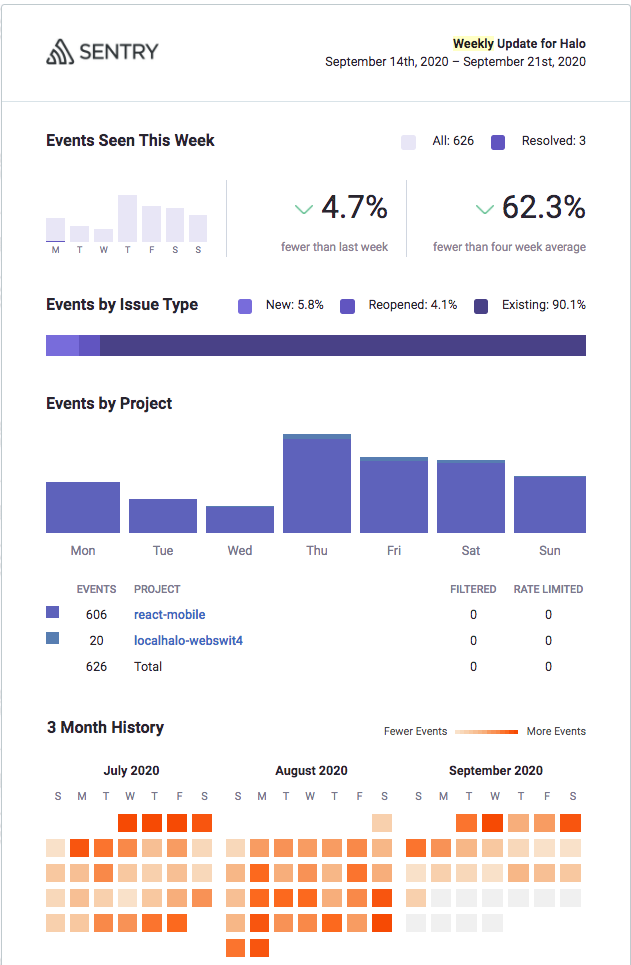
\includegraphics[width=9cm]{images/localhalo/sentry-weekly-report-21-Sep-2020.png}
    \caption{LocalHalo: Sentry weekly report 14 - 21 September 2020}
    \label{fig:localhalo-sentry-weekly-report-21-sep-2020}
\end{figure}

\textbf{Sentry}

MUST-DO Check in Sentry for the various types of error. How actively are the development team reading, reviewing and addressing crashes being reported? 

\begin{figure}[htbp!]
\centering
\begin{minipage}{.5\textwidth}
  \centering
  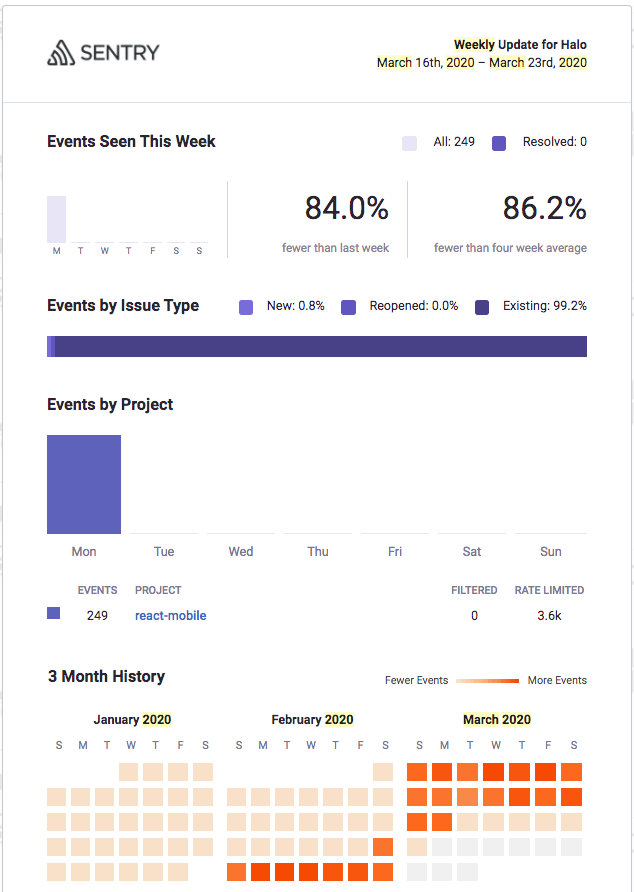
\includegraphics[width=.8\linewidth]{images/localhalo/sentry-weekly-report-16-mar-2020.png}
  \captionof*{figure}{\nth{16} -~\nth{22} March 2020}
  \label{fig:localhalo-sentry-weekly-report-16-mar-2020}
\end{minipage}%
\begin{minipage}{.5\textwidth}
  \centering
  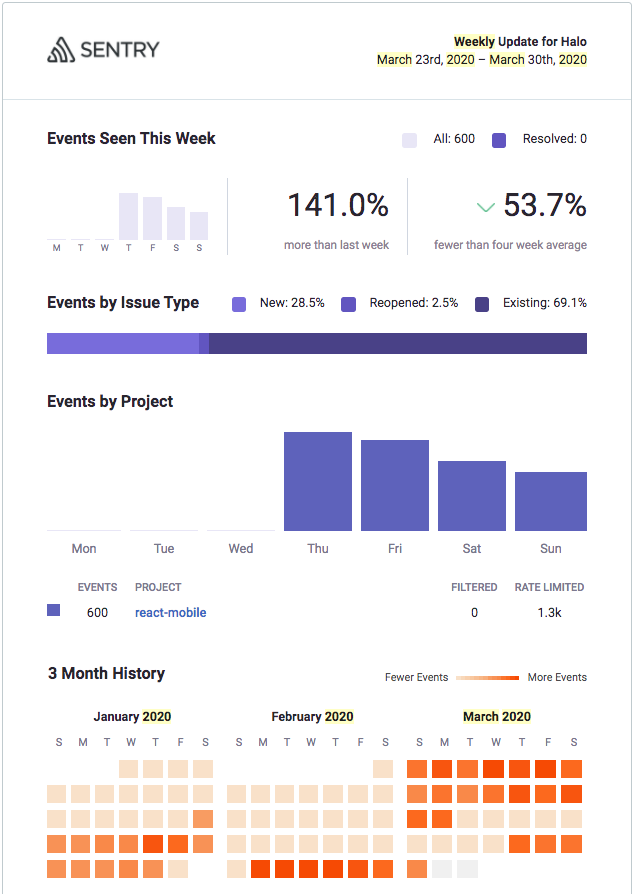
\includegraphics[width=.8\linewidth]{images/localhalo/sentry-weekly-report-23-mar-2020.png}
  \captionof*{figure}{\nth{23} -~\nth{29} March 2020}
  \label{fig:localhalo-sentry-weekly-report-23-mar-2020}
\end{minipage}
    \caption{Missing data reported in Sentry}
    \label{fig:sentry-missing-data-march-2020}
\end{figure}

\begin{comment}


\begin{figure}[htbp!]
    \centering
    %\subfigure[]{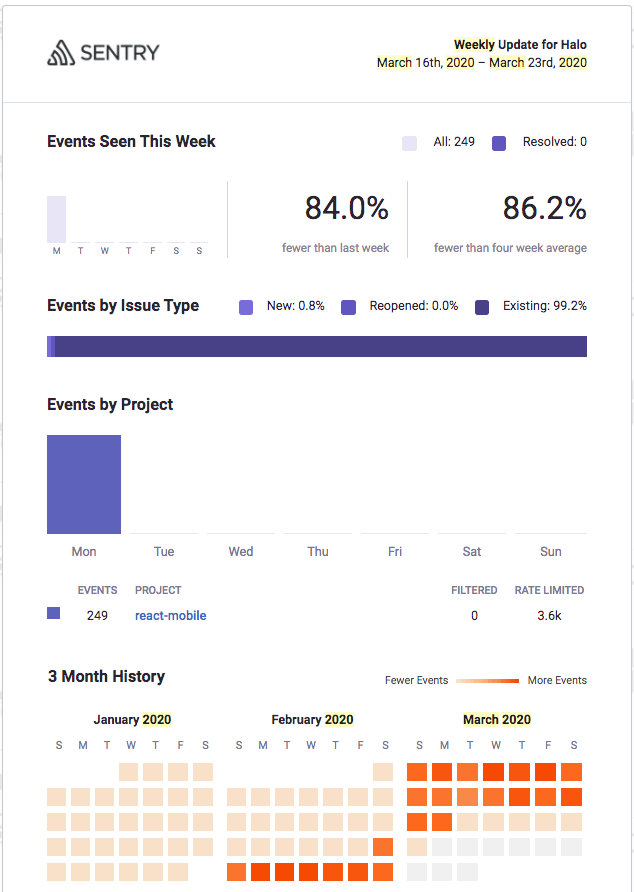
\includegraphics[width=0.4\textwidth]{images/localhalo/sentry-weekly-report-16-mar-2020.png}\caption{\nth{16} -~\nth{22} March 2020}\label{localhalo-sentry-weekly-report-16-mar-2020}}
    \subfigure[]{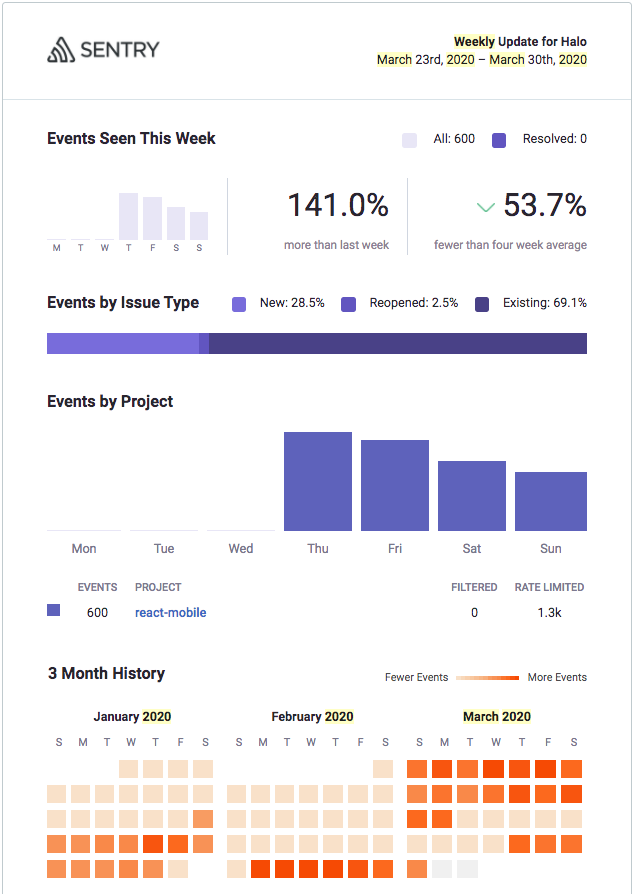
\includegraphics[width=0.4\textwidth]{images/localhalo/sentry-weekly-report-23-mar-2020.png}%\caption{\nth{23} -~\nth{29} March 2020}%\label{localhalo-sentry-weekly-report-23-mar-2020}
    }
    \caption{Missing data reported in Sentry}
    \label{fig:sentry-missing-data-march-2020}
\end{figure}
\end{comment}

%TODO fix the layout of the above figures: try: https://tex.stackexchange.com/questions/37581/latex-figures-side-by-side/37597#37597
Data missing from reports from~\nth{17} March to~\nth{25} March 2020 which affected the statistics around the time of the crashes related to Expo. Figure~\ref{fig:sentry-missing-data-march-2020} illustrates the gap across the two weekly reports. 

SHOULD-DO Consider summarising the crash totals per week. 

\textbf{MUST-DO} write up what we learn from the localhalo case study. external libraries can adversely affect the reliability of apps. Even small development teams can and do use multiple mobile analytics libraries. What can developers learn from the various reports provided by Sentry? How does cross-platform development in react-native affect the app reliability? are there crashes that only occur on Android or iOS? What's the correlation between crashes reported in Android Vitals and Sentry?


\subsection{Summary of Field Reports}
Active and ongoing use. 

%%% Ad-hoc notes from meeting Jakob D. Moonpig
% Business changes including the company's IPO mean the company has cut back on information they're willing to share internally and externally (e.g. for my PhD research).

\clearpage

\section{Corporate engineering case studies}
\label{section-corporate-engineering-case-studies}
\textbf{Relevance}
Brand name corporations with large engineering teams can choose from any of the commercial mobile analytics tools and/or develop their own. They need to deliver software at scale and that scales. They have far larger professional software development teams than any of the other case-studies and face different challenges. They already use multiple mobile analytics tools, their challenge is to harness them consistently and productively to improve the `health' of their software and service to help staunch their loss of users because of software failures. In parallel they aim to launch new features that need to work for millions of users and serve both business-to-business and business-to-consumer users.


\subsection{A major technological corporation}
\textbf{Context} Acceptable use of PII. Fast growth of the team and very rapid initial growth of use of the service. High crash rates led to abandonment by users. 


% A major corporation with millions of paying customers launch a free service in their main territory. Take up is rapid. 

\subsection{Methodology}
Consultant and advisor to the team with access to the key commercial sources of client-side analytics and access to the source code of the Android app and related library project. Worked with one of the product engineering teams for a fast growing product in the covid-19 era of 2020 and beyond.

\textbf{Priorities} data pipelines, ability to query across the many data sources without silos, 

\textbf{Some example issues} multiple analytics tools and data sources incorporated into the software and services, and yet extremely high ANR rates, very high crash rates. DNS error, how the error was discovered. 

\subsection{Lessons learned and/or confirmed}
Not all users of clients update, and a buggy release may leave a large stain on the statistics for the app. As the development team size increases so does the tendency to entropy in the implementation and use of embedded analytics. Furthermore, the team need to consistently check and apply the results of the many and various analytics services if they are to manage and improve the reliability and performance of their software.

The tools need to scale to billions of events per day.

Android Vitals provides a unique source of information, on ANR errors. Microsoft Windows does not offer equivalent reporting to the app developers. %TBD what Apple provides.

Blind spots exist, as do inconsistencies in the various end-to-end data collection and reporting in each analytics offering. 



\subsection{Uber}
MUST-DO write up notes from 14-Jan-2021.

Cite various recent public articles and videos on Uber's engineering practices and team size.


\subsection{Dynamics of sizes of development teams}
Development teams range from one person part-time to many people who work full time on particular mobile apps. A twitter survey that finished on \nth{2} January 2021 had 818 votes; the results are shown in Table~\ref{tab:gergelyorosz_twitter_team_size_survey_02_jan_2021}. %Source \url{https://twitter.com/GergelyOrosz/status/1345288831029956610}. 
The author, Gergley Orosz, asked anyone with more than 20 mobile engineers to add their company name in a reply. At least 22 people did so, they follow in approximate~\footnote{As the contents of answers varied an absolute order is hard to establish.} descending order.

\begin{table}[htbp!]
    \centering
    \begin{tabular}{c|c}
        Mobile app team size &Percent  \\
        Up to 5 devs &53.5\% \\
        5-20         &25.9\% \\
        More than 20 &8.9\% \\
        More than 50 &11.6\% \\
    \end{tabular}
    \caption{Native app mobile development team size~\citep{gergelyorosz2021_twitter_mobile_app_poll}}
    \label{tab:gergelyorosz_twitter_team_size_survey_02_jan_2021}
\end{table}

In addition to the survey respondents with teams Companies with more than 20 engineers include: Uber (100+), % Why is the Uber App So LArge?? https://www.youtube.com/watch?v=zmeCYiD0hnE 
WayFair (100+), Gojek Indonesia (80+ on Android, iOS similar), % 50M+ downloads, 3M6 ratings, a super-app https://play.google.com/store/apps/details?id=com.gojek.app 
Twitter (70+ for iOS, 70+ for Android), Rappi (70 android, 60 iOS), iFood (50+ Android consumer app), Android music app (50+ per mobile platform), Target (80), BumbleEng (40 Android devs, similar for iOS), Xing (30+ for Android), Skyscanner (`~30 per platform'), Garmin (about 30 per platform, excluding those working on internal libraries), `>50 Mercado Libre | nasdaq: Meli', Just Eat (20+ per platform), hotels.com have several subteams - Expedia estimated at 50 per platform, `many native devs at Walmart', unnamed enterprise app 40 Android app developers, 80\% via agencies, `At 
@Falabella\_India we are 29 engineers working on Falabella ecommerce app. 12 are Android Engineers, 13 are iOS Engineers and 4 are QA Engineer.', N26 (`more than 20 ios/android engineers'), 19 in total at thecodeside.com, SoundCloud (`under 20 if you count per platform')~\citep{gergelyorosz2021_twitter_mobile_app_poll}.
%%%%
% COULD-DO cross-reference the development teams with their apps, possibly in tabular format to see if there's a pattern between team size and approximate userbase of the app. Note unless the actual active user counts are available they would need to be estimated based on the installation buckets Google Play Console provides. As I've discovered these counts vary significantly so we'd need to guesstimate and provide error-bars. A bubble chart might be useful.

\subsection{i1}

Crash rates increased inadvertently through changes in the in house networking code paradoxically intended to improve the code quality of the networking related code. One of the changes added a network interceptor (a standard piece of functionality provided by the OkHttp library) to log networking calls and responses. This code inadvertently only worked when the networking response had a `happy path' response. The revised code was code-reviewed and tested as usual. When the app was released with the revised networking code and the rollout into the userbase increased the release management section of Google Play Console reported an increase in crashes, however the rollout was not paused or halted at the time, possibly the reports hadn't been noticed by many in the team at the time? By the time this release was installed on the majority of the userbase the daily crash rate had climbed  to around 10\%, over double the crash rate of previous recent releases.

MUST-DO describe how the networking issues were addressed, automated tests, modified code, new release, steady and ongoing improvement in the measured crash rate. COULD-DO also discuss the distinct yet related changes to the networking code in the separate API codebase.

The experience of the networking crashes are similar to those reported in an Industry report from Apteligent in September 2016 where they found 20\% of crashes were correlated with a network issue at the time. The authors stated the causation figure was closer to 7\% of all crashes on iOS and Android [were related to network-related code]~\citep{apteligent2016_data_report_network_crash_edition}. %See also https://www.slideshare.net/apteligent/apteligent-choosing-the-right-sdks-to-optimize-app-performance-68423213 which restates the crash rate. It also had useful tips on assessing an SDK and the provider of the SDK.

FWIW More information on similar refactoring available in `Legacy Project Refactoring: Handling API Errors with Retrofit2 and RxJava' \url{https://medium.datadriveninvestor.com/legacy-project-refactoring-handling-api-errors-with-retrofit2-and-rxjava-c9f8b23c7673}


\subsection{Some observations in common}
For the larger corporations where the multiple engineering teams combine to develop, maintain and operate mobile apps multiple sources of analytics are used. These often include a mix of external commercial services together with at least one proprietary logging and analytics service. In these examples the organisations see the benefits of integrating their various analytical sub-systems and invest significantly to integrate and streamline the various sources to enable and facilitate consistent reporting across products, platforms, and apps.

\clearpage

\section{Research in logging practices}
\label{section-research-in-logging-practices}
Portions of the contents of this case study have been published in a jointly authored paper published at MOBILESoft 2021~\citep{harty2021_logging_practices_with_mobile_analytics}.

\begin{figure}
    \centering
    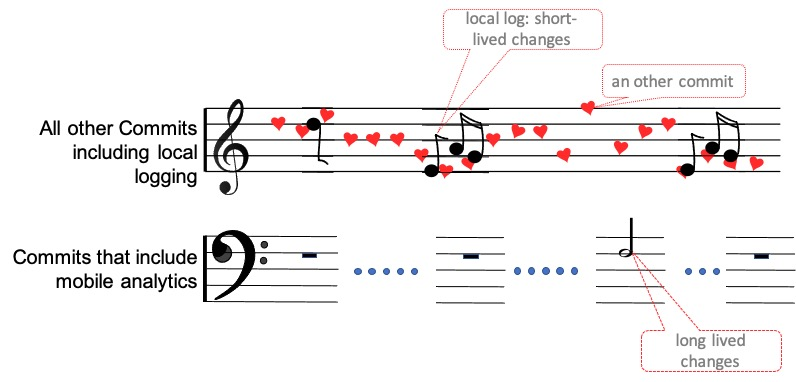
\includegraphics[width=15cm]{images/mobile-analytics-logging/musical-illustration.jpg}
    \caption{Musical representation of commits for local and mobile analytics logging}
    \label{fig:mobile_analytics_logging_musical_illustration}
\end{figure}

This case study investigates commits to various software repositories to determine their composition and characteristics of the frequency of those related to mobile analytics and the contents of the mobile analytics messages implemented in those commits. 

Commits to repositories may be hard to visualise; there is at least one software project that represents commits both visually and through sound, namely \href{https://github.com/debugger22/github-audio}{GitHub Audio} and available online~\url{https://github.audio/}~\footnote{Inspired by \href{http://listen.hatnote.com/\#}{Listen to Wikipedia} with the associated software project~\url{https://github.com/hatnote/listen-to-wikipedia}.} which does so. The patterns of commits this case study detected inspired a way to represent commits, their contents, and the longevity of their contents through music. Figure~\ref{fig:mobile_analytics_logging_musical_illustration} where each commit is represented as a heartbeat. Some include changes to local logging, some include changes to mobile analytics logging and these are represented by musical notes. Commits provide the tempo, the length of the note represented the length a particular change lives for where shorter notes represent short-lived changes, and longer notes represent long-lived changes. 

% The organ music score in https://music.stackexchange.com/questions/24426/what-does-grt-and-sw-mean-in-this-organ-score might be a good basis to develop my musical analogy. 

\subsection*{Rationale}
%\marian{Need to connect this case study with the thesis: what was the goal and show the key contributions. Rationale for this case study. which gave me the chance to look at .... Rationale for the intervention.}

This case study investigates and illustrates how developers have chosen to use mobile analytics to effectively provide remote logging from the field when their application is being used. The case study presents empirical research into characteristics of mobile analytics logging including the density of logging code, the frequency of updates to this code, and also what is being logged. Logging is an endemic practice in software engineering and the realisation that developers have chosen to use mobile analytics effectively for remote logging is relevant in terms of its use for measuring and potentially improving the reliability of their apps.

This case study gave me the chance to look at the historical practices of hundreds of developers of actively maintained Android apps. The goal was to increase understanding of what these developers have used the most popular and prevalent mobile analytics service (Firebase Analytics) for. It also presented an excellent opportunity for international collaboration with a mix of fledgling and highly experienced researchers in areas related to my research.

\textbf{Still TBD} how to weave in, and integrate, the earlier work Joe and I did to analyse local logging and the software we created to help analyse log messages. It was a precursor to the collaborative research and certainly helped inform my thinking and aspects of my collaboration with the rest of the authors, first at the Shonan, and then subsequently in the joint research that led to the MOBILESoft 2021 paper. In my view the work with Joe on log analysis aligns with the case study however none of us actually applied that work to the collaborative case study discussed in this section.

\par\noindent\rule{\textwidth}{0.4pt}

\subsection*{Contributions of this case study}
\begin{itemize}
    \item Insights into the footprint and overhead of what developers of 57 Android apps actively log, together with an understanding that developers of 50 more Android apps chose to simply integrate Firebase into their app and [presumably] rely on the default information Firebase provides them.
    \item An example of collaborative research I helped lead in an area related to my PhD.
    \item Identifying differences between internal and external logs/logging.
    \item A connection established between logging and mobile analytics.
    \item TBC the intersection between using mobile analytics \textit{and} crash reporting.
\end{itemize}


\setminted{fontsize=\small,baselinestretch=1}

\subsection*{Evidence}
  \begin{minted}[
    gobble=4,
    frame=single,
    fontsize=\tiny,
    breaklines=true
  ]{yaml}
    evidence available :
      public reproduction package : \url{https://github.com/mobileanalyticslogs/mobileanalyticslogging}
      local private reproduction : ~/sandbox/apmtracker and~\url{https://github.com/julianharty/research-in-logging-practices}
      co-written-paper : MOBILESoft 2021
      joedocs : various notes.
        \url{https://joedocs.com/julianharty/site/apm-logging-research}
      zoom : various meeting recordings.
      overleaf: drafts and the final paper for MOBILESoft 2021
    evidence-needed : 
      An assessment of which of the 107 projects also incorporate crash analytics.
      Review Luca's list of 8K verified Android apps on GitHub.
      Are any of the 107 apps on f-droid? How many are in the 8K verified Android apps from Luca Pascarella et al.?
  \end{minted}  

\subsection*{ad-hoc, interim, notes}
Notes from Skype call on 14 May 2021 for this case study in particular
\begin{enumerate}
    \item  Clearly separate temporary content from content intended to remain in the thesis.
    \item  Across a collection of apps and their characteristics
    \item  Limit the stuff off message. \textit{The message is to always connect Reliability, Mobile Analytics, and Software Engineering.}
    \item  Explain briefly that F-Droid is an app store that has these characteristics... 
    \item  Check the intersection between the 57 apps and those on F-Droid.
    \item  Commits provide the tempo - helps understand the illustration, the sonification, vs. does the audio help the developers improve their code.
    \item  It's OK to self-plagiarise provided I make this clear to the reader
\end{enumerate}


\subsection{Introduction}
\emph{(Highlight key features of case, similarities and differences w.r.t. other cases);}

This case study provides an additional perspective: that of investigating what various opensource Android developers have used Firebase Analytics for in their Android apps. It complements the development team case studies (where I worked with and/or interviewed the developers) by studying the contents and history of source code of 107 projects. It mines software repositories hosted on~\href{https://github.com/}{GitHub} and compares the use of the foremost mobile analytics SDK (Google's Firebase Analytics) for logging compared to the use of local logging.

Where these apps are in Google Play the developers would already have access to Google Play Console and Android Vitals, yet they have chosen to incorporate an additional analytics library into their app's codebase to log various details. 

Similarities to other case studies include: the projects are for live, actively maintained, Android projects and apps. Mobile Analytics is at the core of the case study. It investigates the use of mobile analytics by the development teams. The research has been collaborative in nature and aims to lead to further research.

We had two primary research questions for this case study:
\begin{enumerate}
    \item What are the characteristics of logging practices with mobile analytics?
    \item What do developers log in mobile analytics?
\end{enumerate}


\subsection{Context}
\emph{(Product/Project overview, Developer characteristics, tools, methods, key challenges for product/project);}

In this section, we present our case study and the results through answering our two research questions.

\noindent \textbf{Subjects.} Our study is based on analyzing 25,611 Java projects used in prior research of logging utilities practices~\cite{boyuanlogutility}. In particular, all the Java projects are obtained from the GHTorrent~\cite{10.5555/2664446.2664449} MySQL dump  (last updated on 2019-06-01). Duplicate (\textit{e.g.} forks and clones) projects were removed as were inactive projects. In order to identify the projects that use Firebase Analytics, we further filtered the projects by searching keyword ``FirebaseAnalytics'' in each project's source code and collected 107 projects. For each of the 107 projects we manually examined whether customised APIs are used by developers for mobile analytics logging. We found 50 of them only collect the default automated metrics generated by Firebase without proactively logging any information. Therefore, our study focuses on the remaining 57 projects where developers intentionally leverage the logging features in Firebase to collect information for their software.

\noindent \textbf{Identifying logging statements.} Initially we followed the same practice as prior research where logging statements are identified based on the Abstract Syntax Tree (AST) and the particular pattern of method invocation of each logging library~\cite{yizengemse,chen2017characterizing}. 
%
However, after manually examining the logging statements, we found \emph{developers often wrap the Firebase APIs in a custom logging class}. In particular, logging using the Firebase API is rather complex where multiple method invocations are often needed to 
log once. Therefore, developers rarely directly call the Firebase APIs to log. Instead, they create wrapper class that provides utility methods that log using the Firebase API.
% This is also hard to decipher.
We manually identified these wrapper classes and their utility methods. These methods were used as keywords to automatically identify the logging statements in their respective project.
%
Specifically, we leveraged srcML to convert source code files to XML files. (Kotlin source files were first renamed from \texttt{*.kt} to \texttt{*.java} which was enough to process them). We then extracted all the invocation calls by using XPath. Then, for each project we used regular expressions to check whether the caller names matched with the corresponding class names we found.


The project was initiated in December 2019 during various breakout sessions I participated in at Shonan Workshop 152~\citep{nii_shonan_workshop_152} where we, a group of researchers, agreed we would like to learn more about mobile analytics being used for logging by mobile apps. The initial group comprised of three late stage PhD students~\footnote{Two of these successfully defended their thesis during this case study.} and two associate professors. We were subsequently joined by an additional early stage PhD candidate who led the initial searches for suitable projects and who also wrote the source code and scripts used to perform the core analysis of these projects.

As one of the professors (\href{https://users.encs.concordia.ca/~shang/}{Weiyi Shang}) had extensive, recent, and relevant experience of two key and related aspects, namely 1) analysis of local logging practices in opensource Android apps~\citep{zeng2019studying_logging_practices_fdroid} and 2) in using the srcML analysis tool we used these to bootstrap our research. Similarly, the GHTorrent offline repository of GitHub projects~\citep{gousios2012_ghtorrent_githubs_data_from_a_firehose} was chosen for the initial selection and filtering of projects based on his recommendation and prior research experience. 


\subsubsection{Methods} 
%GHTorrent records the information of all the projects on GitHub. In the first step, we downloaded the most recent GHTorrent SQL dump and ruled out the projects (projects not in java or kotlin) we didn't need. In the second step, we further filtered these projects with FirebaseAnalytics. The first step was done by a previous master student in our lab, I started my work from the second step.  The GitHub HTTP queries are mainly used for further filtering the projects, the GraphSQL queries are mainly for getting the author information and the commit information etc. so that we can email the authors (we finally decided not to do the survey part so the information is not used). 

\textbf{Identify the projects to analyse}
The first pass was to identify Android apps on F-Droid~\citep{fdroidwebsite} that included Firebase Analytics. F-Droid is a small, alternative to Google Play for Android apps where the apps and the app store are all fully opensourced. There are currently just over 4,000 apps in May 2021~\footnote{Based on summing up the package counts for all the categories~\url{https://f-droid.org/en/packages/}.} % {Connectivity:213,Development:158,Games:378,Graphics:64,Internet:553,Money:109,Multimedia:432,Navigation:203,Phone \& SMS:91,Reading:187,Science \& Education:267,Security:179,Sports \& Health:136,System:545,Theming:166,Time:181,Writing:207} 
% See also https://en.wikipedia.org/wiki/F-Droid for various analysis of f-droid, at the time of writing it was several months out of date.
so it's a miniature app store, yet one that's used relatively frequently by researchers owing to the availability of the source code and visibility into the system and service compared to the Google and Apple app stores.

Only 7 were found to incorporate Firebase Analytics in the F-Droid source projects. We therefore decided to analyse public projects hosted on GitHub which hosts many more Android apps. (Counts vary, ~\citep{geiger2018_a_graph_based_dataset_of_commit_history_of_realworld_android_apps}, identified 8,431 actively maintained, live opensource Android apps matched on Google Play of a far larger set of unique Android apps identified by their package name.)

The most recent GHTorrent SQL dump that was available at the time, from \nth{1} June 2019~\footnote{The dump is available from \url{http://ghtorrent-downloads.ewi.tudelft.nl/mysql/mysql-2019-06-01.tar.gz} it's 102973 MB (source~\url{https://ghtorrent.org/downloads.html}) so best to only download when needed and practical to do so!}. This was filtered in two stages, first to exclude projects not in Java or Kotlin which resulted in 25,611 matches, and then those were filtered to select those that included FirebaseAnalytics (a compound word to match the relevant SDK in the source code) \textit{i.e.} for Firebase Analytics.

\textbf{Selecting active, real-world, apps}
GitHub.com contains a vast range of projects and the nature of git where forks of projects are encouraged and trivial to do meant we needed to filter out duplicates, toy, and inactive projects. Various signals were used to perform the filtering including the number of project stars, the volume and recency of commits, etc. GitHub HTTP queries were mainly used for further filtering the projects.

We also ran ad-hoc queries by searching for the keyword firebaseanalytics directly on GitHub for edification and to help the various authors participate and for sanity checks.
%
An example of the query is \url{https://github.com/search?q=\%22implementation+\%27com.google.firebase\%3Afirebase-analytics\%27\%22&type=Code}. These match a pattern used in \texttt{app/build.gradle} a standard file in virtually all Android projects. Listing~\ref{listing:trashout_ancient_firebaseanalytics_version} provides an example of one of the search results. A quick indication this project is no longer actively maintained is the version number at the end of the line of code, version 15.0.1 of Firebase Analytics was current in Spring of 2018 (as confirmed by the release history for Firebase: \url{https://firebase.google.com/support/release-notes/android#version_1502})~\footnote{Oddly this lists release 15.0.0 and 15.0.2 and does not have an entry for 15.0.1, yet 15.0.1 is found in examples online.}.

\begin{listing}
\begin{minted}[
    gobble=4,
    frame=single,
    fontsize=\tiny,
    breaklines=true
  ]{groovy}
      implementation 'com.google.firebase:firebase-analytics:15.0.1'
\end{minted}
\caption{Source~\href{https://github.com/TrashOut/Android/blob/e897c1c05629f3f5da23516fdfbd24870f773166/app/build.gradle\#L88}{Line 88 of app/build.gradle for TrashOut Android}}
\label{listing:trashout_ancient_firebaseanalytics_version}
\end{listing}
%%%% Note groovy is the language code to use for gradle, see https://pygments.org/docs/lexers/

\textbf{Identify the logging statements}

\begin{listing}
\begin{minted}[
    gobble=2,
    frame=single,
    fontsize=\tiny,
    breaklines=true
  ]{bash}
  % Sanity check of commits for the muzei Android app for messages that mention adding or revising analytics
  git log --oneline | grep -i analytics | grep -v Up | grep -v Merge | grep -v Disable | grep -v Convert | wc -l
\end{minted}
\caption{Bash command as a sanity check for commits mentioning analytics in the muzei Android repo}
\label{listing:sanity_check_muzei_android_commits}
\end{listing}


\textbf{Identify potential contributors to survey}
We performed preliminary analysis to identify the potential candidates for a survey. These include the person who made the first, second, and last commits. The script~\href{https://github.com/mobileanalyticslogs/mobileanalyticslogging/blob/76569d59f0ea6f49f9549433d24ae59dda7fedfd/util/repo\_info\_crawler.py}{util/repo\_info\_crawler.py} also identified the top three contributors to each of the repositories. 

GraphQL queries were mainly used that queried GitHub's GraphQL API~\footnote{\url{https://docs.github.com/en/graphql}} to obtain the author and the commit information \textit{etc.}. 

From an ethics perspective all these details are publicly and freely available \footnote{For example, the contributors for the OneBusAway Android app are available online at~\href{https://github.com/OneBusAway/onebusaway-android/graphs/contributors}{Contribotors to OneBusAway/onebusaway-android}.} and the people involved choose how much personal information to provide and can use pseudonyms, ~\emph{etc.}.

Note: We decided not to do the survey so the information was not used.


\textbf{Establish and maintain coherence across the team}
As a disparate group of individuals, from different cultures, various mother tongues, and working across multiple timezones (from Hong Kong to Quebec) there were multiple opportunities for confusion, misunderstandings, and miscommunication. As a group we therefore focused on establishing and maintaining coherence by having each person work with at least two others, through actively taking and sharing notes, and so on. Furthermore we established a common codebook with total agreement on the contents and the assignment of categories to each of the log lines in the `training set' used to calibrate us as a team and as a coherent group of researchers.  

\textbf{Establish the codebook}


\textbf{Apply the codebook on a larger, representative, sample}


\textbf{Key challenges} included finding suitable projects on f-droid, identifying suitable projects on GitHub, agreeing on the classifications, \href{subsection_srcml_working_with_kotlin_files}{working with Kotlin source files}, and the collaboration in general given the range of locations and timezones of the authors. 

\textbf{Methods for effective collaboration}
As a codicil to the methods section, here is a brief overview of the methods used to collaborate as researchers. 

We used a private GitHub repo for the data analysis and source code until the first paper was written. Overleaf was used as our collaborative editor for academic writing and subsequent publications. In addition two online services were used for written work: 1) google docs for ad-hoc documents and spreadsheets, and 2) \href{https://joedocs.com/}{JoeDocs}~\footnote{JoeDocs was co-created and is subsequently maintained by a friend, collaborator, and colleague - Joseph Reeve. JoeDocs provided a practical alternative to Google Docs, especially during the first lockdown for COVID-19 where various online services were struggling to cope.}. 

A series of meetings used Zoom video calls and many of these calls were recorded with the full agreement of the group so we could review to meetings afterwards, for instance if anyone missed a meeting. Of course, emails were also endemic. I made notes for many of the meetings and these are freely available for our group of researchers.

\subsubsection{Working with Kotlin source files}
\label{subsection_srcml_working_with_kotlin_files}

\begin{listing}
\begin{minted}[
    gobble=2,
    frame=single,
    fontsize=\tiny,
    breaklines=true
  ]{bash}
  # Download and install srcML from their project’s website

  srcml -V
  # 1.0.0 etc.

  srcml --show-language ./main/src/main/java/com/google/android/apps/muzei/MuzeiActivity.kt
  # no visible output

  ln -s  ./main/src/main/java/com/google/android/apps/muzei/MuzeiActivity.kt MuzeiActivity.java

  srcml --show-language MuzeiActivity.java#Java
  srcml MuzeiActivity.java -o MuzeiActivity.xml
  vim MuzeiActivity.*
\end{minted}
\caption{Bash commands to show how srcml can be coerced into analysing Kotlin files}
\label{listing:bash_example_srcml_does_kotlin}
\end{listing}

One of the challenges we encountered was in how to analyse source code written in Kotlin~\footnote{Kotlin is increasingly popular both for new Android apps and many developers are migrating code from Java to Kotlin in existing apps. 
%
Up to date estimates of the growth of Kotlin are available from AppBrain~\href{https://www.appbrain.com/stats/libraries/details/kotlin/kotlin}{Kotlin - Android SDK statistics | AppBrain}, for example.}. 
The software tool we used for this research, \href{https://www.srcml.org/}{srcML}, did not support Kotlin directly at the time of the case study, it only supported C, C++, Java and C\#. Our solution was crude yet appeared to be adequate for the purposes of our research; we created symbolic links for each Kotlin source file where the link has a \texttt{.java} extension. Listing~\ref{listing:bash_example_srcml_does_kotlin} illustrates the approach. We checked the XML files that srcML generated for these files together with the results of the regular expression matches to confirm this approach was sufficient~\footnote{Details about srcML including the XML it generates are available on the project's \href{https://www.srcml.org/about.html}{About} page}.

\subsection{Findings and Results}
\textit{(Describe what you did with analytics in the context of the case);} 



\begin{figure}[htbp!]
\centering
\begin{minipage}{.5\textwidth}
  \centering
  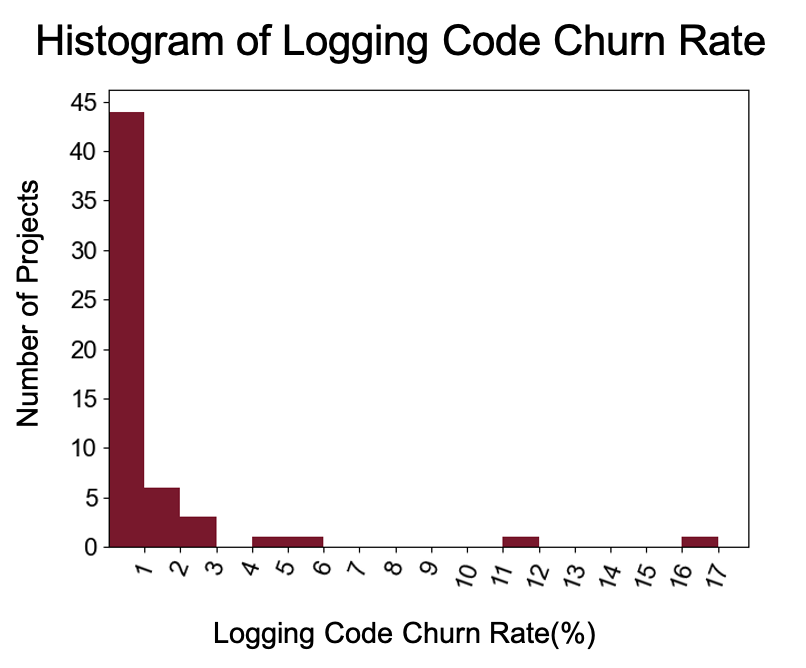
\includegraphics[width=.8\linewidth]{images/mobile-analytics-logging/logging-churn-rate.png}
  \captionof*{figure}{Churn}
  \label{fig:logging-churn-rate}
\end{minipage}%
\begin{minipage}{.5\textwidth}
  \centering
  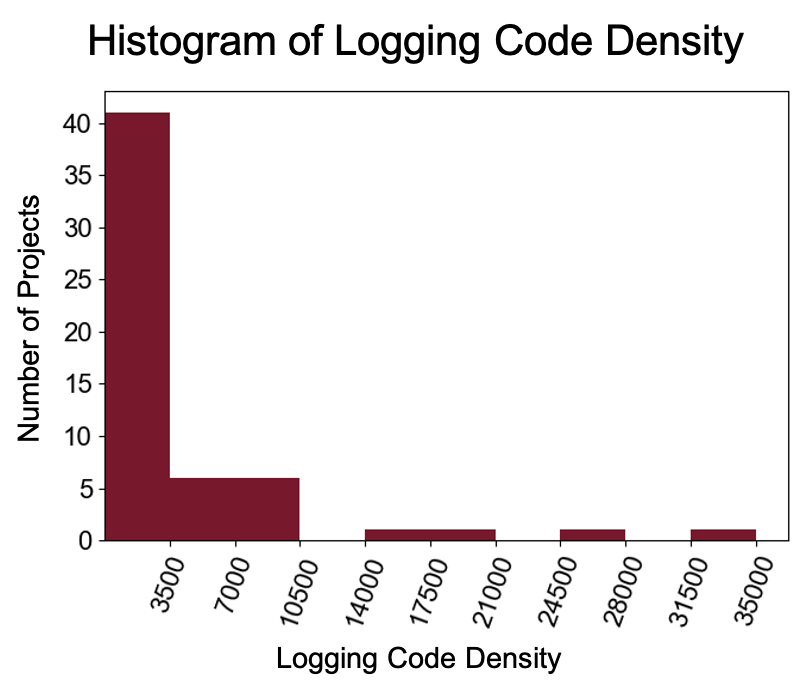
\includegraphics[width=.8\linewidth]{images/mobile-analytics-logging/logging-code-density.png}
  \captionof*{figure}{Density}
  \label{fig:logging-code-density}
\end{minipage}
    \caption{Characteristics of logging}
    \label{fig:logging_rq_1}
\end{figure}

\begin{figure}
    \centering
    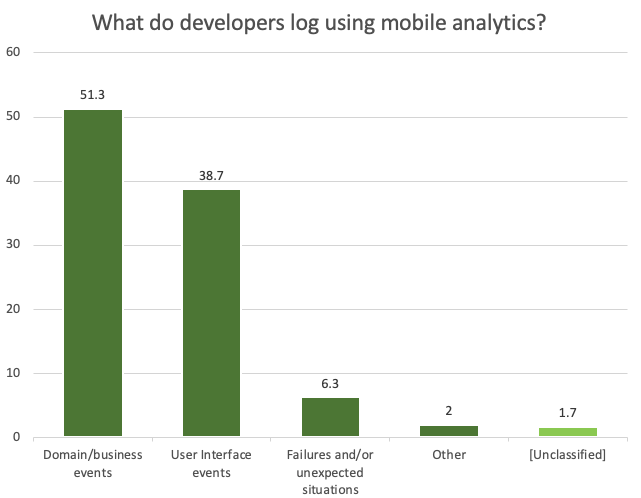
\includegraphics[width=15cm]{images/mobile-analytics-logging/graph-for-research-question-2.png}
    \caption{What is being logged}
    \label{fig:logging_rq_2}
\end{figure}


\begin{listing}
\begin{minted}[
    gobble=4,
    frame=single,
    fontsize=\tiny,
    breaklines=true
  ]{kotlin}
      private fun configureLogging() {
        if (BuildConfig.DEBUG) Timber.plant(Timber.DebugTree())
    }
\end{minted}
\caption{Source~\href{https://github.com/duckduckgo/Android/blob/2f3d42be6a972551c2330daccba6ff4039e1c1a8/app/src/main/java/com/duckduckgo/app/global/DuckDuckGoApplication.kt\#L177-L179}{Lines 177-179 of DuckDuckGoApplication.kt}}
\label{listing:duckduckgo_timber_debug_logging}
\end{listing}

The short source code snippet in Listing~\ref{listing:duckduckgo_timber_debug_logging} provides an example of how developers can choose to vary, or control, the behaviour of the logging for particular builds of their app.


\subsubsection{SmartNavi}
I followed up with one of the 57 projects, the \href{https://smartnavi.app/home}{smartnavi app}~\footnote{The follow-up was triggered by me noticing some problems with a Google website that redirected to an old URL for the project which was now used for insalubrious content. I chose to alert both Google and the project owner so they could address any issues.}.


\textit{The following raw notes are from one of my email updates, on \nth{28} July 2020}

I had my call with Christian Henke who created the project. Here are various notes that are pertinent to our joint research into logging.
\begin{itemize}

    \item The project uses crash reporting (to catch, report, and analyse crashes) and mobile analytics (to try to ascertain where users do and don't use the app). In terms of our coding his use mainly focuses on events generated when users interact with his app.
    \item The app is mature (5+ years) and originally had analytics de developed himself using MySQL, etc. to record the events. He did this mainly to learn about the topic, he was a bachelors|masters student at the time.
    \item Over the years he's used Firebase and Google Analytics mainly for tracking the popularity and use of the app's features. One of the key challenges for this app in his estimation is helping users who don't understand GPS, etc. why the app may be relevant to them. It saves battery life because of the ways it tracks movement, and is mainly intended for people moving at walking pace (rather than in high-speed vehicles).
    \item He also uses Firebase tools to perform A/B experiments related to tutorials and their usability and effectiveness.
    \item He spent a lot of time a year or so ago where he actively focused on fixing crashes being reported in Fabric Crashlytics (since superseded by Firebase Crashlytics). The few crashes that remain are ones either too impractical to investigate (e.g. on a few unbranded low-end Android devices he has no access to) or in a third-party library that only occurs again on a few unusual devices.
    \item The app can run in the background and provide GPS services to other apps e.g. to Google Maps. This has some interesting challenges where Android on various devices and in various conditions may suspend some background activities automatically. If analytics could help track how the background activity is working (and when it's no longer running) that might be very helpful to him and enable him to improve the app's behaviours when run in the background.
    \item He's not proactively working on the app currently. He may spend more time on it soon if he perceives there are new users/use cases for the app. Separately to our research I may help find one or two projects that would be motivating for him e.g. related to mapping Tanzania.
    \item He does coach students at his old university in Germany who are studying marketing. They do various practical exercises to help them gain better marketing skills.
\end{itemize}

We've agreed that there's little more to be gained from asking more about his current quiescent use of analytics since he only checks the analytics infrequently in Firebase (he checked it while we were talking, previously it was around 8 weeks ago he thought). He is happy for others to collaborate on the project, to use it, etc.

\subsection{Outcomes} 
\textit{(Describe the outcomes resulting from the intervention); }


\subsection{Discussion} 
\textit{(Explore what these outcomes mean for the use of analytics in mobile software more generally)}

This case study found the developers of these 57 apps used Mobile Analytics sparsely and the relevant source code was long-lived. Furthermore, what developers chose to log using Firebase differed materially from what similar developers chose to log locally in their codebases. The combination of these findings are worth comparing with the various industrial case studies and these comparisons will be covered later in this thesis %MUST_DO and then add cross-reference link here.  

In hindsight, only finding 7 apps use that firebase logging in F-Droid was a paradox. They were paradoxically too few for the research to be material and too many as F-Droid state they do not accept any apps with Firebase or other non-open Analytics SDKs. The inclusion policy of F-Droid effectively excludes any apps that use Firebase (which they list explicitly as a blocker, along with Crashlytics.)~\url{https://f-droid.org/en/docs/Inclusion_Policy/}. The lack of Firebase Analytics in F-Droid is almost the inverse of what commercial developers do in their Android apps, where over 62\% of all apps include Firebase Analytics, and over 90\% of the top applications do.


\begin{itemize}
    \item Threats to validity include: opensource projects not being very representative of commercial apps; our method where we relied on prior work for our comparisons; use of basic regular expressions; use of srcml that doesn't support Kotlin.
    \item It's an open question whether the opensource developers are using Firebase analytics for similar purposes to the purposes identified in our research. This can be cross-correlated with the interview with Jakob D. where they used Firebase Analytics to capture runtime issues. Admittedly a tiny sample of 4 responses replied to Maurício Aniche's request on Twitter~\url{https://twitter.com/mauricioaniche/status/1250687381914750976} %A copy of the tweet and replies is stored in my misc references folder.
    \begin{itemize}
        \item Pedro Pessoa \href{https://twitter.com/pedpess}{@pedpess} Apr 16, 2020 Replying to @mauricioaniche \emph{``Depends... Usually, critical parts of the biz. For instance, if I can order something from the app, I wanna know if the order succeeded or failed and why... For pure native, I was using Firebase - Crashlytics. Lately, for React Native, Sentry."}
        \item Marabesi Personal computerFlag of Brazil \href{https://twitter.com/MatheusMarabesi}{@MatheusMarabesi} Apr 16, 2020 Replying to @mauricioaniche \emph{``Sentry/bugsnag"}
        \item Robson Soares Amorim \href{https://twitter.com/AmorimRob}{@AmorimRob} Apr 16, 2020 Replying to  @mauricioaniche \emph{``Currently, using App Center to track logs from crashs and custom errors messages in try catchs blocks, personalized events (user clicked on button save, for example). Also, the analytics data provided is very useful for viewing new version adoptions, user session time, devices .."}
        \item Roman Sirokov \href{https://twitter.com/RSirokov}{@RSirokov} Apr 16, 2020 Replying to  @mauricioaniche \emph{``@Firebase has a lot of extremely helpful cross-platform tools; starting from detailed crashlytics, going to app’s performance metrics and user analytics. It’s also possible to implement custom events."}
    \end{itemize}
\end{itemize}

Both this case study and the related work may suffer from the Streetlight effect~\citep{wikipedia_streetlight_effect}, where we research where we can based on sources that are easier to obtain.

\subsection*{Further Work related to this case study}
Further work can be summed up as: ask the devs, concurrent analysis of all the forms of logging, understanding context, and better tooling.

\textbf{Ask the developers:} as mentioned earlier, with one exception, we did not discuss the source code with the authors. We had planned to survey the developers and we believe there would still be merit in doing so to obtain their perspective, experiences, and insights into their use of Firebase Analytics.

\textbf{Concurrent analysis of all logging} This research built on closely-related and relatively recent analysis of similar opensource Android projects. This approach enabled the team to accelerate the initial work and identify broad differences between how Android opensource developers used local and mobile analytics logging. However, by not comparing both local and mobile analytics logging in the same codebases at the same time may have led to inaccuracies in the comparisons. Concurrent analysis of all the forms of logging in the same repos at the same time would help to reduce the scope for inaccuracies and may lead to additional insights.

\textbf{Understanding context}

\textbf{Signal strengths} \textit{c.f. ``On the Naturalness and Localness of Software Logs"} MSR 2021

\textbf{Better tooling} There are several alternative approaches to querying GitHub including the pydriller project (described in~\citep{spadini2018_pydriller}), GitHub's GraphQL API~\footnote{\url{https://docs.github.com/en/graphql}}, and others. These may improve the filtering and selection process. There is also another dataset of verified opensource Android apps on GitHub, ~\href{https://androidtimemachine.github.io/}{AndroidTimeMachine}, described in~\citep{geiger2018_a_graph_based_dataset_of_commit_history_of_realworld_android_apps}. This was co-authored by one of the collaborators for this case study. Unlike our work, theirs includes metadata extracted from Google Play Store; details of their matching and data retrieval process are documented online~\url{https://androidtimemachine.github.io/dataset/} and their implementation is also freely available~\url{https://github.com/AndroidTimeMachine/open_source_android_apps}. Their approach could be used to improve our assessment of liveness and validity of the source repositories, and it might also accelerate aspects of the data collection and filtering.
% To get started, they provide a guide and a docker container https://androidtimemachine.github.io/guide/

Furthermore there are various code analysis tools including: LGTM~\footnote{\url{https://lgtm.com/help/lgtm/customizing-code-extraction}} which provide ways to query codebases for specific calls, and CodeScene which tracks the history of changes in the codebase. These may provide more streamlined and production-refined approaches to analysing the code. These would augment rather than replace the value of asking the developers for their perspectives and insights into their choices in selecting and using mobile analytics to monitor reliability and additional software qualities. 


%%%%%%%%%%%%%%%%%%%%%%%%%%%%%%%%%%%%%%%%%%%%%%%%%%%%%%%%%%%%%%%%%%%%%%%%
\par\noindent\rule{\textwidth}{0.4pt}
~\textbf{Earlier material follows}

Logging and mobile analytics intersect with each other, particularly in terms of how they are implemented and in using them to record aspects of the runtime behaviour of software. Previous case studies in this thesis focused on the use and application of various forms of mobile analytics, this section focuses on some of the details of the implementation of logging and the use of mobile analytics to provide a form of remote logging. 

Here we cover:
\begin{itemize}
    \item analysis of logging practices via Firebase Analytics in 107 opensource Android apps,
    \item tools and utilities developed to facilitate the capture and testing of logging in Android apps,
    \item followed by a discussion the design and testing of logging pertaining to Android apps.
\end{itemize}

Logging orients to line-item details and analytics to patterns in what has been logged when the data is aggregated.

\subsection{TODO Materials to incorporate}
\textit{This subsection is to remind me of my various sources for this case study. This entire subsection needs removing once I've done so.}
\begin{itemize}
    \item My draft paper on improving logging.
    \item The MOBILESoft 2021 paper, under review currently.
    \item Various notes in `Notes' on my macbook account.
    \item Bits and pieces related to Shonan Meeting 152. The report provides a useful reminder. Note, for my hysteresis concept we can also add the adaption and application of enterprise tools e.g. using ELK stack.  
\end{itemize}

%After covering various aspects of logging in proprietary apps and codebases, this section addresses three topics with a common focus on logging and logging tools available in opensource projects. It covers two aspects, with a subsequent discussion on the design and testing of logging:

As we learn to program we also enjoy seeing the program output things to show it's doing something under our control, when we run the program we see messages being output, when we don't run it, we don't - concomitant variation in action!~\citep{mill1884system}. Listing~\ref{code:basic_example} is a representative example of the sort of program some of us would have written in BASIC, equivalent output statements exist in many programming languages. Examples to say `Hello World' are available in 28 programming languages~\citep{helloworld2017}. 

% https://www.overleaf.com/learn/latex/Code_Highlighting_with_minted
\begin{listing}
\caption{A representative first BASIC program} \label{code:basic_example}
\begin{minted}{basic}
10 cls
20 print "Hello, world!"
30 sleep
40 end
\end{minted}
Source: \href{https://en.wikibooks.org/wiki/BASIC_Programming/Beginning_BASIC/Your_First_Program}{en.wikibooks.org/wiki/BASIC\_Programming/Beginning\_BASIC/Your\_First\_Program}
\end{listing}

Programmers continue to write and use output statements to observe aspects of what a program is doing, the values of variables, and so on. This includes programmers who develop mobile apps. They can use core components in a programming language, such as a \texttt{printf\{'...'\}} statement, logging libraries, such as \texttt{Log.w\{'...'\}} from the core \mintinline{java}|Android.util.Log|
library, custom logging libraries such as timber, and proprietary libraries. They can also use Mobile Analytics libraries for logging purposes which is what led to this case study.
% https://tex.stackexchange.com/questions/45756/inline-code-and-short-verb-with-minted

Mobile platforms include an operating system that runs on the device; both Android and iOS are based on UNIX. UNIX includes three standard terminal I/O devices: \texttt{stdin}, \texttt{stdout}, and \texttt{stderr}. Of interest here are \texttt{stdout} and \texttt{stderr} which are both output devices, that output text and errors respectively. Developers can therefore use these in their programs, albeit the platform providers (Google and Apple) recommend developers use logging libraries instead. These I/O devices can be redirected the log files on the devices as various people note.

\textbf{Android} includes: comparing ways to redirect \texttt{stdout} to logcat [the standard Android log]~\citep{krysmanski2012_so_redirect-stdout-to-logcat-in-android-NDK, rcdailey2018_ndk_redirect_to_logcats}, and an elegant solution for native code is described in~\citep{tsiombikas2014_native_NDK_stdio_to_android_log}.

\textbf{iOS} includes: 

By default the output of programs are local to the computer the program runs on. This characteristic limits the ability for programmers to observe or analyse the outputs, they need to be local and see the logs as they are generated. 
%
When programs run remotely from the developer they cannot see the logs directly. Many tools exist for collecting and analysing logs from servers and systems, conversely few tools exist to obtain logs from end-user device, which include their smartphones and tablets. Nonetheless, runtime logs are still of interest to developers of mobile apps both for local debugging (generally pre-release) and for remote analysis.



\subsection{How do developers of opensource Android apps use Firebase Analytics?}
\begin{enumerate}
    \item Analysis of third-party opensource Android apps that incorporate Firebase Analytics.
    \item Tools we created to facilitate the testing and analysis of logging by Android developers.
    \item Discussion in methods to improve the effectiveness of logging and the analysis of log messages generated by apps.
\end{enumerate}

Logging is an integral part of the software development process, ranging from sometimes seemingly random print statements to using fully featured software libraries and sophisticated software systems to transfer, replicate, store and analyze log data. Logs are also important developer aids for diagnosing problems and errors, with many app developers collect crash logs for their app from end-user devices - some even ask users for permission to send crash logs when problems occur.  This use of logging is particularly important for mobile software development, where developers need to understand the difference between between effects of the runtime environment, such as poor connectivity, from behaviours of the app when handling the various runtime conditions.

When developers incorporate mobile analytics in their apps, what do they use them for? 

In earlier case studies in this thesis several commercial developers shared their practices informally. This case study complements their insights by analysing 107 opensource Android projects that use Google's Firebase Analytics (the most popular and prevalent in-app analytics tool) to answer two research questions:
\begin{enumerate}
    \item What are the characteristics of logging practices with mobile analytics?
    \item What do developers log with mobile analytics?
\end{enumerate}

This research was performed jointly with an international group of researchers, all-bar-one, met at the~\textit{\nth{152 }NII Shonan meeting~\citep{nii_shonan_workshop_152}} where a group of us agreed to investigate the use of logging in mobile applications as a follow-up activity. We wrote and submitted our first paper in October 2020 where I am the first author. The paper is currently under review. The materials are available as an opensource project at \url{https://github.com/mobileanalyticslogs/mobileanalyticslogging/}.



Early research explored ways developers of opensource Android apps use local logging, a complementary and oft used approach intended to help developers learn more about how their app behaves locally at run-time. MUST-DO provide context either here or in the related works chapter.



MUST-DO continue to write up our post-shonan paper.



\subsubsection{Tacit/default use of analytics}
50 of the 107 codebases studied ... expand with contents from the collaborative research post Shonan. Cross-link my material on tacit logging here.

\subsection{Tools to facilitate capture and testing of logging}

\begin{itemize}
    \item \href{https://github.com/ISNIT0/log-searcher}{\textbf{Log Searcher}}:
    \item \href{https://github.com/ISNIT0/logcat-filter}{\textbf{Logcat Filter}}:
    \item \href{https://github.com/ISNIT0/log-complexity-comparison}{\textbf{Log Complexity Comparison}}:
    \item \href{https://github.com/ISNIT0/AndroidLogAssert}{\textbf{Android Log Assert}}:
    \item \href{https://github.com/ISNIT0/AndroidCrashDummy}{\textbf{Android Crash Dummy}}:
\end{itemize}



\subsection{Discussion on practical aspects for the design, incorporation, and testing of logging} \label{apx:practical-aspects-for-design-and-incorporation-of-logging}
%This appendix introduces various practical aspects of incorporation of mobile analytics that are not necessary to understand the overall approach. The intention is to help those who would be actively involved in the concepts and approach described in the core thesis.
This introduces germane aspects of the design and incorporation of logging...



\subsection{Designing logging}
Unstructured logging can serve immediate needs, for instance to trace code execution or display the value of a variable at run-time. The resulting entries into a log file have limited value in terms of longer term analysis and they may also be harder to identify, filter, and lack relevant content for such analysis.

In the domain of logging both business and research consider logging design important and valuable. 

Storage and transmission of log entries. Sematext provides opensource libraries for Android~\citep{github2020_sematext_logsene_android} and iOS.

Controllable logging: Developers can optionally provide facilities to control the amount of logging that is performed by the app. The well-established K-9 Mail Android app includes optional debug logging that users can activate to help developers diagnose problems and errors~\citep{github2020_k9mail_logging_errors}. A good example of this feature being used is issue 2705 \emph{``Deleted mail from inbox is doubled in trash directory"} on their GitHub site where various users contributed logs and additional information~\citep{github2017_k9mail_issue_2705}. Out of interest, the issue took 20 months to address and multiple contributions before the development team determined the cause, according to the updates in the issue. The project team uses this facility extensively; by \nth{23} December 2020 they had 11 open and 128 closed issues that included the keyword~\href{https://github.com/k9mail/k-9/issues?utf8=\%E2\%9C\%93\&q=is\%3Aissue\%20is\%3Aopen\%20loggingerrors\%20}{loggingerrors}.
% Note: in 2017 the project has 30 open issues and 39 closed, which reference the LoggingErrors wiki page. https://github.com/k9mail/k-9/issues?utf8=%E2%9C%93&q=is%3Aissue%20is%3Aopen%20loggingerrors%20 Some issues are waiting for logging to be provided, others include the requested logcat output.

Materials to incorporate on designing logging:
\begin{itemize}
    \item Retrace from Stackify: Logging meets monitoring. Full lifecycle APM.~\url{https://stackify.com/}
    \begin{itemize}
        \item \url{https://docs.stackify.com/docs/error-and-logs} Logging Rate, Top Errors, Recent Errors, Top Error Chart, Error Rates in dev, test and production.
        \item Application Performance: Slow Pages, Performance Breakdown, Slow Query, Server Performance, Satisfaction Breakdown.~\url{https://docs.stackify.com/docs/application-performance-widgets}
        \item Monitoring and Metrics, App Score:~\href{https://docs.stackify.com/docs/app-score-widgets}{https:// docs.stackify.com/docs/app-score-widgets}.
        \item Centralized Logging: 
        \item Filters, Fields and Tags, and Querying logs:~\url{https://docs.stackify.com/docs/logs-dashboard}. Monitoring logs. 
    \end{itemize}Control Which Logs are Sent to Stackify; ~\texttt{Enrich.WithProperty};~\texttt{stackifyLogger.ForContext}~\url{https://docs.stackify.com/docs/errors-and-logs-serilog}. \emph{``Our .NET libraries automatically handle batching, compressing, queuing, throttling, and error retry logic for uploading your application logs."}\url{https://docs.stackify.com/docs/errors-and-logs-net-supported-frameworks}. \url{https://docs.stackify.com/docs/troubleshoot-errors-and-logs-net-configurations} 4 steps to troubleshooting logging to Stackify's systems. And possibly use the App Score somewhere else in the thesis?~\url{https://docs.stackify.com/docs/appscore}
\end{itemize}

Implementation choices: 

\subsection{Testing logging}
Unit testing of logging to date has not been widely available as a core capability of the logging libraries. There are several possible approaches to asserting the logging is as expected, these include recording the log output \emph{within} the software \emph{i.e.} in memory, and checking what has been written to an actual log [file]. The first approach is described in \citep{altindag2020_unit_testing_log_messages_made_easy} and made available as an opensource project called LogCaptor~\citep{log-captor-github-project}. The second approach was implemented jointly by myself and Joseph Reeve and made available as an opensource project~\citep{android_log_assert}. Both these approaches assert that what was intended to be in the log actually appears there. At the time of writing, the LogCaptor includes richer examples. Our work supports the standard Android logging API in addition to custom logging libraries. As both projects are opensourced and have permissive licenses there is the opportunity to improve either or both of them and for cross-fertilisation.

\begin{comment}
\begin{itemize}
    \item \url{https://cran.r-project.org/web/packages/logger/vignettes/Intro.html} and the related more detailed references~\url{https://daroczig.github.io/logger/articles/customize_logger.html} and \url{https://daroczig.github.io/logger/articles/anatomy.html} which has a very clear figure~\footnote{\url{https://github.com/daroczig/logger/blob/master/vignettes/logger_structure.svg}} representing how logging is implemented.
\end{itemize}
\end{comment}

\clearpage

\section{A tools provider's perspective: Iterative.ly}
\label{section-tool-providers-perspective}
\label{section-iteratively-case-study}
The use of mobile analytics extends beyond the development role in a team or organisation. Software tools should also serve the project rather than being the master of it. ~\citep{budgen1993_case_tools_masters_or_servants} raises a similar issue of whether CASE tools are masters or servants. There is a significant risk that development teams lose control of the data, and/or are constrained by the policies, implementation, and so on of a particular tool provider. Companies including Iteratively, Avo, and Segment aim to provide aspects of: freedom of choice and the ability to choose, cross team alignment and visibility of the use of embedded (in-app) analytics, and compliance. Here, Iteratively is included as a mini case-study of what one of these companies is doing to help development teams in their use of embedded (in-app) mobile analytics.

%Cross team tracking and alignment on the use of embedded (in-app) mobile analytics 

%Introduce the company: location, age, type of business, etc. Information freely given with permission to use it generally, including for research purposes.
Iteratively was founded on \nth{20} February 2019 and based in Seattle, Washington State, USA by two experienced co-founders. They contacted me in May 2020 as they were interested in my perspective and research into mobile analytics. %Sources include: https://iterative.ly/about/ https://www.crunchbase.com/organization/iteratively
%
Subsequently, they kindly agreed to contribute to this research as a small case study of a startup aiming to develop products to help development teams improve their use of mobile analytics. They provided all information is freely given with permission to use it generally, including for research purposes.

This research case study include these research methods: semi-structured interviews, a walk-through of the tools and service, collaborative verbal discussions and various written materials.

Their service is self-described as ``GitHub for your analytics", providing a versioned schema registry for analytics events~\footnote{Source: a non-public document used with permission.}.
%
Their value proposition: a versioned schema for web and mobile analytics. Tools that generate the client-side SDK that developers then include in their apps. They use lint tools to verify that events have been instrumented correctly. At runtime their SDK validates event payloads match the schema to help enforce data quality. They provide tools that help detect some forms of PII with the aim of helping improve legal compliance.  

Relevance to the research in the thesis: tools to help design and validate the analytics content. A whitebox insight into an analytics provider who also develop and provide tools to help organisations improve their use of mobile and web analytics. 


\subsection{Related work}
- Mention similar work avo.app
- segment.io - indicates the growth and relevance of mobile analytics as a market, of addressing data ownership and freedom of choice of analytics implementations. 

\subsection{Their market research}
MUST-DO expand this section, mainly to cover key points in their early market research and the relevance to the research in this thesis.

What leading edge businesses value in their analytics tools? (10 dots voting examples, see Figure~\ref{tab:10dots_voting_iteratively}), their early market research (see the first notion.io document.)


Dot voting is a simple voting exercise where each participant has a finite number of dots they can vote with to prioritise a set of choices~\citep{18f_dot_voting}. Dot voting is used in many software development teams who use Agile software development practices, and offers easy and lightweight voting of ideas~\citep{nngroup_dot_voting}. There are criticisms of the technique, for instance where poorly designed options split votes, where people vote tactically, or where people appropriate and use dots from others~\citep{dotmocracy}. The approach used by iteratively mitigates against these concerns through the design and implementation of the voting. 

Iteratively's method uses a video call with screen sharing. Each participant has already agreed to take part in the research exercise which includes the ten dots voting as part of a semi-structured interview. They are presented with the prepared template `Spend 10 coins', as illustrated in Figure~\ref{fig:iteratively-spend-10-dots}. The interviewer explains each item in order until each of them have been explained. Some interviewees allocate the coins (dots) early others wait until the end of the explanation.


\begin{figure}[htbp!]
    \centering
    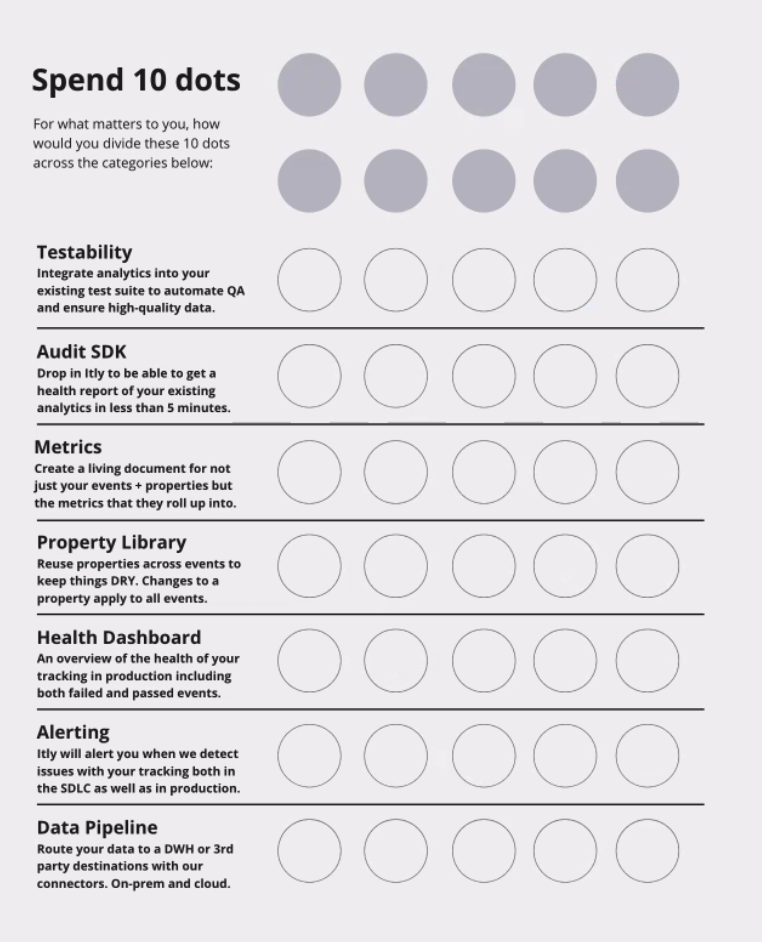
\includegraphics[width=10cm]{images/iteratively/spend-10-dots.png}
    \caption{Interatively spend 10 dots}
    \label{fig:iteratively-spend-10-dots}
\end{figure}

According to Iteratively the votes are helpful, and the discussions around the topics more so.  Figure~\ref{fig:iteratively-dot-voting-example} is an example where the votes have been cast. 

\begin{figure}[htbp!]
    \centering
    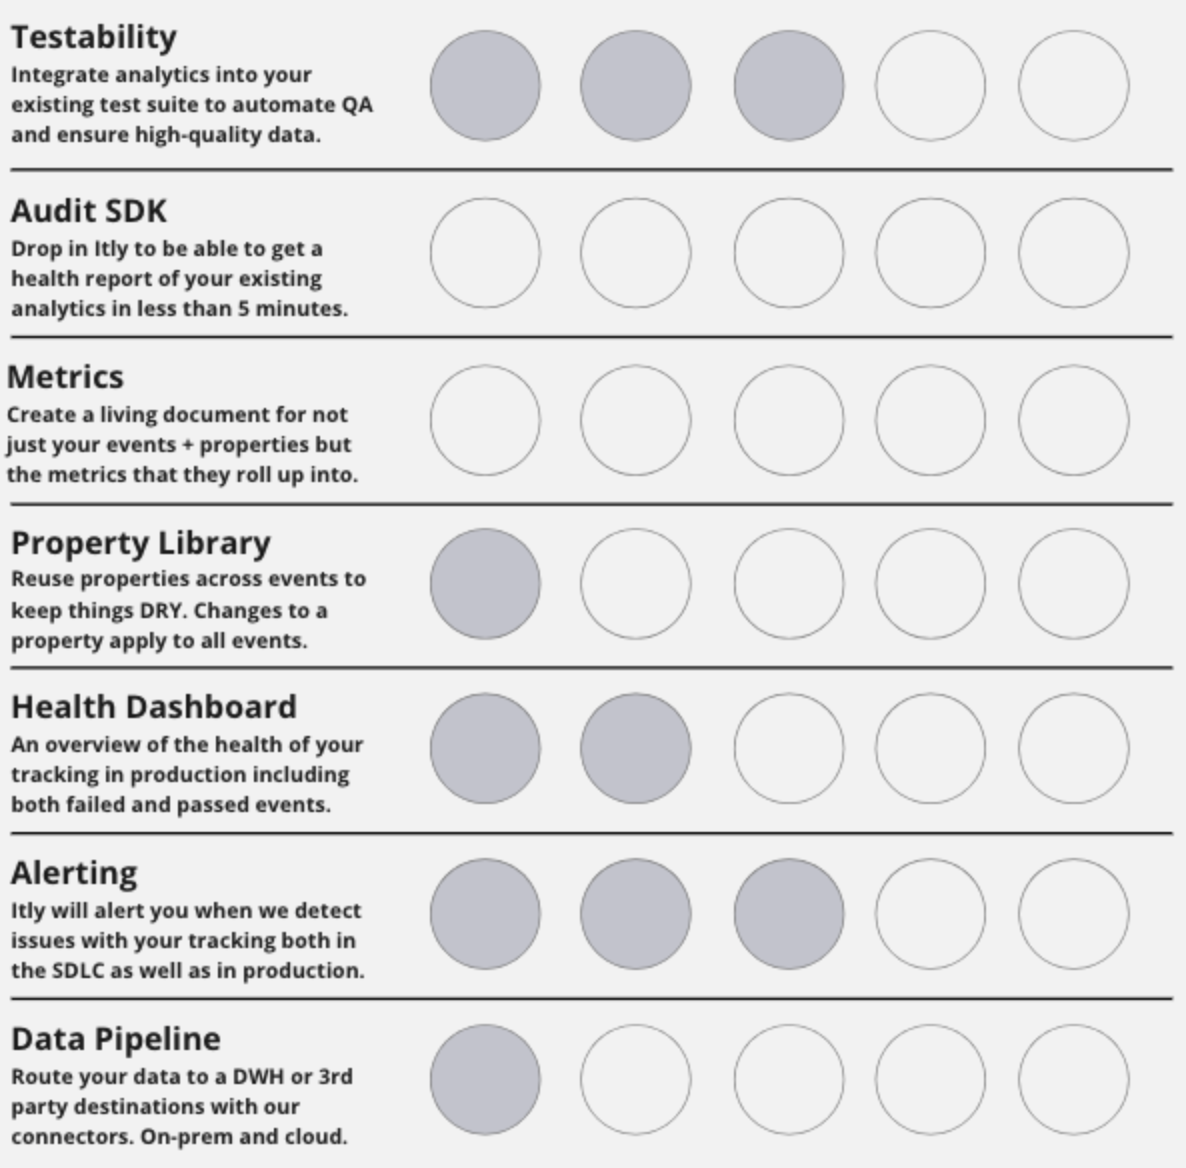
\includegraphics[width=10cm]{images/iteratively/dot-voting-example.png}
    \caption{Iteratively dot voting example}
    \label{fig:iteratively-dot-voting-example}
\end{figure}


Seven candidate topics were used, here are the exact wordings of each topic description:
\begin{enumerate}
    \item \textbf{Testability}: Integrate analytics into your existing test suite to automate QA and ensure high-quality data.
    \item \textbf{Audit SDK}: Drop in itly\footnote{itly: Iteratively.} to be able to get a health report of your existing analytics in less than 5 minutes.
    \item \textbf{Metrics}: Create a living document for not just your events + properties but the metrics they roll up into.
    \item \textbf{Property Library}: Reuse properties across events to keep things DRY. Changes to a property apply to all events.
    \item \textbf{Health Dashboard}: An overview of the health of your tracking in production including both failed and passed events.
    \item \textbf{Alerting}: Itly will alert you when we detect issues with your tracking both in the SDLC\footnote{SDLC: Software Development Life Cycle.} as well as in production.
    \item \textbf{Data Pipeline}: Route your data to a DWH\footnote{DWH: Data Warehouse.} or 3rd party destinations with our connectors. On-prem~\footnote{On-prem: On premise.} and cloud.
\end{enumerate}
These topics were chosen to help Iteratively with planning their product roadmap. They also provide a useful context and perspective for the research into using mobile analytics from product and data engineering perspectives. With one exception, all the participants actively use analytics in their software and have expressed an interest in improving their approach into incorporating and using analytics in their apps.

\begin{table}[htbp!]
 
    \centering
    \small
    \setlength{\tabcolsep}{4pt} %% default is 6pt
    %% With thanks to http://tex.my/how-to-deal-with-wide-tables/ for the \tabcolsep tip
    \begin{tabular}{lr|rrrrrrrrrrrrrr}
    % SHOULD-DO Added column span over the participants, reduce the heavy lines on the table.
                     &Sum &A  &B  &C  &D  &E  &F  &G  &H  &I  &J &K &L &M &N\\
    \hline     
    Testability         &30 &3  &3  &3  &1  &   &3  &3  &1  &5  &3 &  &3 &1 &1\\
    Audit SDK           &25 &   &2  &   &   &2  &2  &3  &1  &2  &1 &3 &3 &5 &1\\
    Metrics             &6  &   &   &   &   &   &1  &   &   &   &  &  &1 &3 &1\\
    Property library    &21 &1  &3  &3  &2  &3  &2  &1  &   &   &1 &1 &1 &  &3\\
    Health Dashboard    &17 &2  &   &2  &   &3  &   &2  &2  &   &2 &2 &  &1 &1\\
    Alerting            &18 &3  &2  &   &2  &   &2  &   &4  &   &3 &  &1 &  &1\\
    Data Pipeline       &18 &1  &   &2  &   &2  &   &1  &2  &3  &  &4 &1 &  &2\\
         
    \end{tabular}
    \caption{10 dots voting Iteratively market research}
    \label{tab:10dots_voting_iteratively}

\end{table}
% My spreadsheet https://docs.google.com/spreadsheets/d/1Acti8klc6JvLu_NAR7t7cC8XdMHx-FIkfSHcqt_srwc/edit#gid=0 
% Source from iterative.ly's miro board https://miro.com/app/board/o9J_kujB-Y4=/ 

The first ten sets of dot votes rank the choices as follows: Testability (25), Property Library (16), Alerting (16), Audit SDK (13), Health Dashboard (13), Data Pipeline (11), and lastly Metrics (1). The next three sets of dot votes cement testability as the \#1 ranking, they also bump up auditing the use of the SDK to second place in the rankings, and even metrics gets a boost to 5 votes in total. 

With 14 sets of votes, the ranking is still volatile and the scores unlikely to be sufficiently robust to depend on. Nonetheless several indications are starting to emerge. 
These votes indicate testability is the most desired property for designing and implementing analytics where the analytics can help shape and drive automated testing of software based on production usage characteristics. Auditing of the SDK is in a strong second place, to provide an immediate health check of the existing analytics. Participants who use Iteratively's services score property library highly as they have experienced the value in this capability. Alerting when issues are detected with the tracking in the SDLC and production ties in joint fourth place with the data pipeline. Data pipeline is more important than it may appear, as some of the respondents professed they preferred alternatives to using Iteratively to provide the data pipeline. The interviews indicated that data pipelines are more important than the score indicates.

The seven topics were chosen quickly and not necessarily intended to be comprehensive. One omission we discussed is the area that encompasses: privacy, Personally Identifiable Information (PII), and compliance, nonetheless these are believed to be important to Iteratively's current and potential customers and an area they are actively working on.

\subsection{Evaluation of their service}
SHOULD-DO apply their tooling for an Android app for an existing app and discuss the effects of using their tooling and service. % Possibly do this with Joe Reeve to include his perspective as he transitions from outsider to insider at the company?

\subsection{Indications of where mobile analytics is heading}
Iteratively and several companies with similar value propositions indicate several potential trends in the use of mobile analytics. These trends include: mobile analytics is now subject to quality criteria, where organisations seek mechanisms to help them integrate mobile analytics as a first-class citizen in app development, potentially at least as valuable as some features in their apps. Also there is a need and a desire to use and manage mobile analytics effectively, including ownership and management of the data that is collected by the many and various mobile analytics tools. 

% Call notes with Patrick Fri 30th April 2021 30 mins, 16:00 BST
% He's keen to read my thesis and provide feedback.
% He's fine with him and with Joe providing details and me picking Joe's brains about Iteratively and the products. 
% He's also keen to give back in terms of the help and advice I've provided

\clearpage

\section{Some additional examples}
\label{section-some-examples}
Here are some examples of investigating failures discovered by using mobile analytics. Some details have been revised or removed to protect the source, these changes do not affect the core message of the example.

\subsection{Errors in network-related code}

Tell the story: the initial problem, the initial 'fix' and the resulting effects. Further analysis and the improved fixes. Final results.

\textbf{Issue}

\textbf{Discovery of the issue}

\textbf{Bug investigation}

\textbf{Establishing the traffic characteristics}

\subsubsection{Tools and techniques when working on networking code}

\begin{figure}
    \centering
    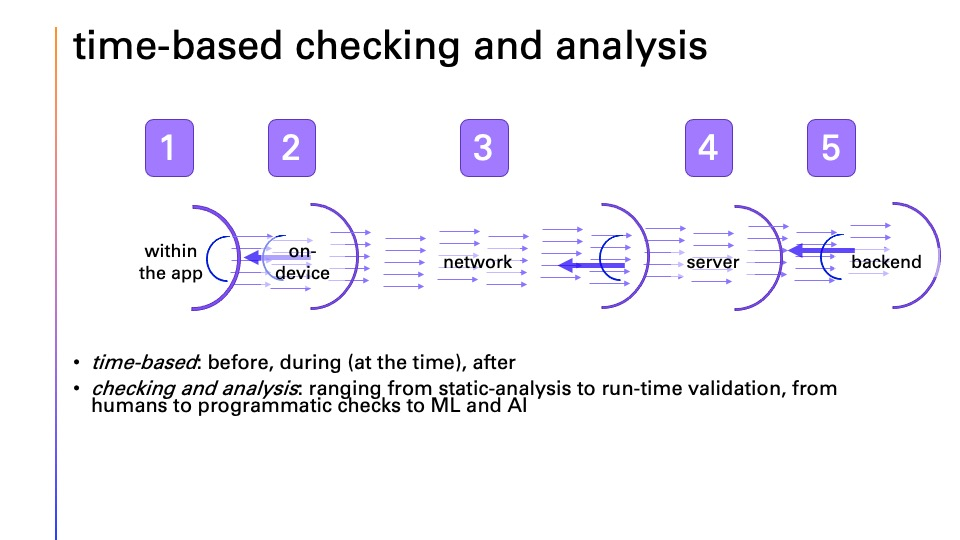
\includegraphics[width=15cm]{images/my/time-based-checking-and-analysis.jpg}
    \caption{Time-based checking and analysis}
    \label{fig:my_timebased-checking-and-analysis}
\end{figure}

Figure~\ref{fig:my_timebased-checking-and-analysis} illustrates five distinct zones where the behaviour of network IO may be checked and potentially controlled. There are a range of mechanisms and tools available to both check and control the network IO. These include:

\begin{itemize}
    \item mock servers that can run within the system under test TODO add link to OkHttp MockWebServer,
    \item external local servers, such as Qontract, 
    \item network monitors and traffic interceptors,
    \item modifying the configuration of the primary servers, such as nginx, to return particular results and behaviours,
    \item making similar modification in back-end systems and services.
\end{itemize}

\textbf{Method} 
\begin{itemize}
    \item Manual code comprehension
    \item Experiments with using protocol server. Network traffic routing, techniques for redirecting the intended destination.  Modifications to the protocol server.
    \item OkHttp source code and reviewed their automated tests and testing.
    \item Create pure JVM minimum example to decouple from Android dependencies.
    \item Use mock web server and custom configuration of the mocks to reproduce the crash in the JVM.
    \item Devise, implement and test a suitable fix.
    \item Port the automated tests, support code, and implementation back to the Android codebase. Determine and implement support for JUNIT 5 test execution on Android using a third-party, opensource utility.
    \item Prove the bug can also be reproduced using the automated tests with the current application codebase.
    \item Port the fix and integrate it into the Android app.
    \item Perform code review on the changes, create pull request, another code review, merge the changes.
\end{itemize}

We also discovered other flaws in the closely related code that would lead to crashes. Devised a tiny change to the ordering of three code statements that would address the flaw. This change was excluded from the next release for various internal reasons. Released a new version of the app with the improvements, crash rate reduced over 5x. Observed that the flaw we had discovered was actually being exposed in production (now the major crash had been addressed this was easier to observe. Consider, was error masking as a factor?). Awaiting a rollout of the fix for the ordering of the interceptors. 


\textbf{Results: bug reproduction}

\textbf{Results: improving the code}

\textbf{Results: effects in production}


\clearpage

\section{Summary of Case Studies}~\label{section-summary-of-case-studies}
MUST-DO revise and update this summary close to submitting the thesis - when the main canon of the work is closed; i.e. when there are no new case studies likely to be added.

Summary of bugs
Bugs will reach production. They vary on their visibility, effects, and ease of reproduction. Some may be latent for long periods. Their effects may also vary, with some affecting a small number of users, others may have a more widespread effect across a population. Some will be destructive to the end user's experiences while others may be virtually unnoticeable. 





The case studies includes a useful range of Android apps developed by independent teams using a variety of programming languages, mindsets, objectives, and constraints. In each team they learned to actively focus on stability metrics as reported in various technology-facing analytics tools, and the developers continue to see the merit of doing so on an ongoing basis.

Developers want to improve their software however their ongoing use of usage analytics ranges from infrequent to integrating it in their working practices. Moonpig and Kiwix Android are two projects where they actively engage with mobile analytics. They have chosen different approaches, Moonpig incorporated in-app mobile analytics into their app and use the platform level analytics as a secondary source of information. Kiwix Android relies on the platform level analytics. Of these Moonpig is able to address issues more quickly and target failures accurately through the additional data they receive from Firebase Analytics. 

Ease-of-use and richness of the reports are key factors and led several of the teams to choose reports from App Center, Fabric, and Firebase over Google Play Console.

Being able to actively manage and track failures across and between systems is also an important factor for at least some of the teams. As examples, the Greentech team actively cross-reference crashes with their ticketing system, as do both the commercial teams, one going so far as to automatically create tickets for newly discovered crashes in their apps.


Testability is a cross-cutting concern which applies throughout the development and operational aspects of mobile app development. Examples include the ease (or otherwise) of being able to reproduce reported issues, testability of the analytics libraries, tools, and services, and testability of changes to the app pre-release to try and ascertain whether the stability of the app will improve once it has been launched and deployed to a large portion of the userbase.






Integration and streamlining become increasingly important as the userbase and teams grow. The case studies alone are insufficient to provide quantitative trends, nonetheless they align with my experience across multiple large organisations in the USA, Europe, and beyond. The ad-hoc survey by Orosz provides examples of tens of organisations who have development teams of at least 20+, 50+, and even 100+ developers on the team for an app.


Many of these large teams will have apps that include crash and in-app analytics, and they are likely to have multiple people accessing and using analytics reports. They may include multiple people contributing code related to using the respective crash and in-app analytics APIs which may lead to gaps and inconsistencies in the application of these tools unless the entire team works hard to maintain consistency in their practices. Tools, such as those provided by Iterative.ly (a tool vendor introduced in one of the case studies in this thesis) aim to help provide coherence, clarity and consistence in the use of mobile analytics. Software development style guides, software quality utilities, and productive code reviews, may also help to establish, maintain and even improve the practices. In the opensource projects evaluated in one of the case studies \textbf{MUST-DO} write that up and extend this section... the developers were found to update their use of mobile analytics for logging less frequently than other aspects of their code.


% Also, COULD-DO For the 107 Android apps we reviewed post Shonan #152, are there any patterns between the use of Firebase Analytics and the active developer userbase? i.e. how many significant contributors does each of these projects have?
\clearpage